%% ---------------------------------------------------------------------------
%% Thesis.tex -- MAIN FILE (the one that you compile with LaTeX)
%% ---------------------------------------------------------------------------
% https://www.sharelatex.com/templates/thesis/graduate-thesis/
% Set up the document
% Use the "Thesis" style, based on the ECS Thesis style by Steve Gunn
% use the draft option to print overfull hbox
% TODO: change to twoside when done
% oneside = one side printing and screen reading
% twoside = for double side printing
\documentclass[a4paper,11pt,twoside]{Thesis}
% Location of the graphics files (set up for graphics to be in PDF format)
\graphicspath{Figures/}

% Include any extra LaTeX packages required
% Use biblatex to bibliography management
\usepackage[
  backend=biber,
  %style=numeric,% [1], [25], etc
  style=alphabetic,%[CF04], [Carv14], etc
  %sorting=ynt, %year,name,title
  sorting=anyt, %alphabetic label,name,year,title
  hyperref=true,
  maxbibnames=15,
  maxcitenames=3,
  maxalphanames=5, % with 5 authors, use the 5 initials as label
  sortcites=true,
]{biblatex}
% show a raised + for label with more than 1 author
\renewcommand*{\labelalphaothers}{$^+$}
\addbibresource{Bibliography.bib}
\DefineBibliographyStrings{english}{%
  bibliography = {References}, % show References on TOC
}
% vim-latex's completion only works when the bibliography command is present
%\bibliography{Bibliography}
% Todonotes wrongly placed in the margin
%TODO: remove this by the end? WTF is this for?
\setlength{\marginparwidth}{2cm}

\usepackage{tikz-cd} % for commutative diagrams
\usepackage{paralist} % for inline lists
%% ---------------------------------------------------------------------------
\begin{document}
% Begin Roman style (i, ii, iii, iv...) page numbering
\frontmatter

% Set up the Title Page
\title  {A practical validation of Homomorphic Message Authentication schemes}
\authors  {{Nuno Tiago Ferreira de Carvalho}}
% Do not change this here, instead these must be set in the "Thesis.cls" file,
% please look through it instead
\addresses  {\groupname\\\deptname\\\univname}
\date       {\today}
\subject    {}
\keywords   {}

\maketitle
%% ---------------------------------------------------------------------------

% It is better to have smaller font and larger line spacing than the other way
% round
\setstretch{1.5}

% Define the page headers using the FancyHdr package and set up for one-sided
% printing
% Clears all page headers and footers
\fancyhead{}
% Sets the right side header to show the page number
\rhead{\thepage}
% Clears the left side page header
\lhead{}

% Finally, use the "fancy" page style to implement the FancyHdr headers
\pagestyle{fancy}

%% ---------------------------------------------------------------------------
% The Declaration page
% No headers or footers for the following pages
%\pagestyle{empty}
% relative to .build/ folder
%\includepdf[frame=false,scale=0.935,offset=57 -110]{../../documents/parecer.pdf}
%% Declaration ended, now start a new page
%\clearpage

%% ---------------------------------------------------------------------------
% The "Funny Quote Page"
% No headers or footers for the following pages
%\pagestyle{empty}
%
%\null\vfill
%% Now comes the "Funny Quote", written in italics
%\textit{``Write a funny quote here.''}
%
%\begin{flushright}
%If the quote is taken from someone, their name goes here
%\end{flushright}
%
%\vfill\vfill\vfill\vfill\vfill\vfill\null
%\clearpage  % Funny Quote page ended, start a new page

% Reset the line-spacing to 1.5 for body text (if it has changed)
%\setstretch{1.5}

%% ---------------------------------------------------------------------------
% The Abstract Page
% Add the "Abstract" page entry to the Contents
\addtotoc{Abstract}
\abstractpage{
  % Add a gap in the Contents, for aesthetics. NO
  %\addtocontents{toc}{\vspace{1em}}
  
  \begin{abstract}{english}
  \noindent Currently, cloud computing is very appealing because it allows the
  user to outsource his data so it can later be accessed from multiple devices.
  The user can also delegate to the cloud computing service provider some,
  possibly complex, operations on the outsourced data. Since this service
  provider may not always be trusted, it is necessary to not only preserve the
  privacy but also to enforce the authenticity of the outsourced data.  Lately,
  a lot of work was put on solving the first problem, specially after the
  introduction of the first Fully Homomorphic Encryption scheme. In this work
  we will focus on the latter, namely on the use of Homomorphic Message
  Authentication primitives. We will evaluate the current available solutions,
  their functionality and their security. Finally, we will provide an
  implementation of one of these schemes in order to verify if they are indeed
  practical.
\end{abstract}

%\begin{abstract}{portuges}
%  \noindent Currently, cloud computing is very appealing because it allows the user to
%  outsource his data so it can later be accessed from multiple devices. The user
%  can also delegate to the cloud computing service provider some, possibly
%  complex, operations on the outsourced data. Since this service provider may not
%  always be trusted, it is necessary to not only preserve the privacy but also to
%  enforce the authenticity of the outsourced data.
%  Lately, a lot of work was put on solving the first problem, specially after the
%  introduction of the first Fully Homomorphic Encryption scheme. In this work we
%  will focus on the latter, namely on the use of Homomorphic Message
%  Authentication primitives. We will evaluate the current available solutions,
%  their functionality and their security. Finally, we will provide an
%  implementation of these schemes in order to verify if they are indeed
%  practical, and a comparison between them.
%\end{abstract}


}
% Abstract ended, start a new page
\cleardoublepage

%% ---------------------------------------------------------------------------
% The Acknowledgements page, for thanking everyone
\pagestyle{empty}
\acknowledgements{
% Add a gap in the Contents, for aesthetics.
\addtocontents{toc}{\vspace{1em}}

\vspace{3.5em}

To my supervisor, Professor Manuel Bernardo Barbosa, for the great opportunity,
all the guidance and all the suggestions that lead me here, many thanks.

To Professor Dario Catalano, for receiving me in Catania and for all the
precious help and advises given during my stay. A special thanks to Professor
Mario di Raimondo for the practical suggestions.

To all my friends, specially the ones who kept up with me during these last few
stressing weeks. A special mention to the ones who somehow were with me during
these last 6 years of studying.

To my friends in Catania, specially the people from the residenza, for
understanding the reason of my absence so many times.

Lastly, but not least, to my parents, Domingos and Maria, and to my sister,
Joana, without whom I wouldn't be here, a profound and sincere thank you for
providing me the with the necessary conditions and support to be here now.
\vfill

\begin{otherlanguage}{portuges}
  Este trabalho foi apoiado pelo Projeto Smartgrids - NORTE-07-0124-FEDER-000056,
  cofinanciado pelo Programa Operacional Regional do Norte (ON.2 – O Novo Norte),
  ao abrigo do Quadro de Referência Estratégico Nacional (QREN), através do Fundo
  Europeu de Desenvolvimento Regional (FEDER).
\end{otherlanguage}

}
% End of the Acknowledgements
\clearpage
%% ---------------------------------------------------------------------------

% The page style headers have been "empty" all this time, now use the "fancy"
% headers as defined before to bring them back
\pagestyle{fancy}
%% ---------------------------------------------------------------------------
% Set the left side page header to "Contents"
\lhead{\emph{Contents}}
% Write out the Table of Contents
\tableofcontents

%TODO: add list of figures and list of tables and abbreviations
%% ---------------------------------------------------------------------------
% Set the left side page header to "List if Figures"
%\lhead{\emph{List of Figures}}
%% Write out the List of Figures
%\listoffigures

%% ---------------------------------------------------------------------------
% Set the left side page header to "List of Tables"
%\lhead{\emph{List of Tables}}
%% Write out the List of Tables
%\listoftables

%% ---------------------------------------------------------------------------
% Set the line spacing to 1.5, this makes the following tables easier to read
\setstretch{1.5}
% Start a new page
\clearpage
% Set the left side page header to "Abbreviations"
\lhead{\emph{Abbreviations}}
\printnomenclature

%% ---------------------------------------------------------------------------
%% End of the pre-able, contents and lists of things
%% Begin the Dedication page
%\clearpage
%
%% Return the line spacing back to 1.5
%\setstretch{1.5}
%
%% Page style needs to be empty for this page
%\pagestyle{empty}
%\dedicatory{For/Dedicated to/To my\ldots}
%
%% Add a gap in the Contents, for aesthetics
%\addtocontents{toc}{\vspace{2em}}

%% ---------------------------------------------------------------------------
% Begin normal, numeric (1,2,3...) page numbering
\mainmatter

% Return the page headers back to the "fancy" style
\pagestyle{fancy}
% Clears all page headers and footers
\fancyhead{}
\fancyhead[LE,RO]{\thepage}
\fancyhead[RE]{\emph{\leftmark}}
\fancyhead[LO]{\emph{\rightmark}}
% Include the chapters of the thesis, as separate files
% Just uncomment the lines as you write the chapters

%% ---------------------------------------------------------------------------
% INTRODUCTION
%% ---------------------------------------------------------------------------
\chapter{Introduction}\label{chap:intro}
A cloud computing provider allows a user to lease computing and storage
resources from remote computers that are far more powerful than the user's.
This enables her to perform operations over (some portion of) outsourced data
that is remotely stored and then only the results of these operations are
returned to the user. However, the current infrastructures of cloud computing
services do not provide any security against untrusted cloud operators, making
them unsuitable for storing sensitive information such as medical, financial or
any personal records.

A possible solution to this problem is the use of homomorphic cryptography.
This concept was first presented by \textcite{rivest:adleman:dertouzos:1978}
about 30 years ago. However, it remained an open problem until recently, when
the first truly homomorphic schemes were proposed. With these schemes it became
possible to perform computations on encrypted data such that the cloud
computing provider does not have access to the decrypted information, therefore
preserving \emph{privacy} of the outsourced data. The first \nom{FHE}{Fully
Homomorphic Encryption} scheme was proposed in a ground-breaking work by
\textcite{gentry:2009:FHE}. His scheme allows the computation of arbitrary
computations over encrypted data without being able to decrypt. Unfortunately
it is not yet practical, but several small improvements have been proposed
which could lead it to be practical in the near future.

But, and not only in the context of cloud computing, it is also important to
guarantee the \emph{authenticity} of the computations performed on the
outsourced data. FHE schemes by itself only guarantee privacy, and not
authenticity. To do so, two main goals need to be fulfilled: \emph{security}
and \emph{efficiency}. Security guarantees that the server is able to ``prove''
the correctness of the delegated computation. Efficiency means that the user is
able to efficiently check the proof by requiring far less resources than those
needed to execute the delegated computation (including both computation and
communication).

%% ---------------------------------------------------------------------------
% MOTIVATION
%% ---------------------------------------------------------------------------
\section{Motivation}
To guarantee authenticity for computations on outsourced data a new set of
homomorphic primitives were defined: homomorphic signatures (asymmetric
setting) and homomorphic message authenticators (symmetric setting).

The first notions of homomorphic signatures were introduced around 15 years ago
by \textcite{rivest:micali:chari:rabin:2001}, and then
\textcite{johnson:molnar:song:wagner:2002} presented a more complete
definition. An homomorphic signature scheme allows a user to generate
signatures $\sigmaSpace{1}{k}$ on messages $\mSpace{1}{k}$ so that later anyone
(without the private signing key) can compute a signature $\sigma'$ that is
valid for the value $m' = f(\mSpace{1}{k})$. Also, it allows anyone that holds
the public verification key to verify the results.
\textcite{boneh:freeman:2011} constructed a scheme that evaluates multivariate
polynomials on previously signed data, but they also stated that the
construction of a fully homomorphic signatures scheme remains an open problem.

The secret key analogue of homomorphic signatures are homomorphic message
authenticators (homomorphic \nom{MAC}{Message Authentication Code}s for short)
that were introduced by \textcite{gennaro:wichs:2012}. In this setting, there
is a public evaluation key and a secret key shared by Alice and Bob, which is
used to authenticate some messages $\mSpace{1}{k}$. Then, anybody who has the
public evaluation key can compute a short tag $\sigma$ that certifies the value
$y = f(\mSpace{1}{k})$ as the output of $f$. Notice that $\sigma$ does not
simply authenticate $y$ out of context, it only certifies it as the output of
a specific $f$. Later, Bob can verify that $y$ is indeed the output of
$f(\mSpace{1}{k})$ without even knowing the value of the messages.
%
\textcite{gennaro:wichs:2012} also presented a construction with support for
arbitrary computations, a fully homomorphic MAC, but its security is based on
a weaker model (the adversary cannot ask for verification queries, only for
authentication queries).

To overcome this problem, and relying on much of the work from
\citeauthor{gennaro:wichs:2012}, \textcite{catalano:fiore:2013} constructed a
very simple and efficient scheme with support for a more restricted class of
computations. Furthermore, its security is based on a stronger model with
support for multiple verification queries.
%
But both of these constructions suffered from a common problem: the
verification algorithm runs in time proportional to the size of the function.
The scheme from \textcite{backes:fiore:reischuk:2013} tries to solve this
problem, and it is the first homomorphic MAC scheme with efficient (amortized)
verification.

\begin{comment}
As for the homomorphic MAC schemes, they all rely on the theory of arithmetic
circuits for the computation of functions over some messages. Simply put, an
arithmetic circuit over a field $\bbF$ and a set of variables $X
= \{\tauSpace{1}{k}\}$, is a directed acyclic graph with the following
properties.  Each node in the graph is called \emph{gate}. Gates with in-degree
0 are called \emph{input} gates while gates with out-degree 0 are called
\emph{output} gates. Each input gate is labeled by either a \emph{variable} or
a \emph{constant}. A variable input gate is labeled with a binary string
$\tau_i$ and can take arbitrary values in $\bbF$. A constant input gate is
labeled with some constant $c$ and can only take some fixed value $c \in \bbF$.
Each \emph{internal} gate (gates with in/out-degree greater than 0) is labeled
by either $+$ or $\times$, sum and product gates, respectively. The \emph{size}
of the circuit is the number of its gates. The \emph{depth} is the length of
the longest path from input to output.

Polynomials are evaluated with arithmetic circuits as follows: input gates
compute the polynomial defined by their labels. Sum gates compute the
polynomial obtained by the sum of the (two) polynomials on their incoming
wires, while product gates compute the product of the two polynomials on their
incoming wires. The output of the circuit is the value contained on the
outgoing wire of the output gate.
\end{comment}

%% ---------------------------------------------------------------------------
% OBJECTIVES
%% ---------------------------------------------------------------------------
\section{Objectives}
We intend to study the current homomorphic MAC constructions in order to better
understand their strengths and pitfalls. Having realized what those are, we
want to implement one of these constructions, \textcite{catalano:fiore:2013} to
be more precise. The reason we ignore the implementation of
\textcite{gennaro:wichs:2012} is because of its reduced security and because it
relies heavily on lattice based techniques, which are not yet efficient.

Our main goal is then to measure the overhead introduced by the homomorphic
evaluation of \cite{catalano:fiore:2013}. In practical terms, what we intend to
measure is the amount of extra work that the external server must do to
homomorphically compute the function in comparison to a normal computation.

We will also measure the complexity of all the other operations of
\textcite{catalano:fiore:2013} in order to check if it is already practical.

\begin{comment}
In this work we will mainly focus on homomorphic MAC schemes, and all of them
rely on the theory of arithmetic circuits.
%
In practical terms, it is important to stress that arithmetic circuits should
be seen as computing \emph{specific} polynomials in $\bbF[x]$ rather than
functions $\bbF^{|x|}$ to $\bbF$. Essentially, one is interested in the formal
computation of polynomials rather than the functions that these polynomials
define. This is because a function may be expressed by a polynomial in several
ways, while, in general, a polynomial defines a unique function.\footnote{A
  good example of this case is the zero function. $f = x^2 + x$ is clearly not
the zero function, unless it is in $\bbF_2$.}

The scheme from \textcite{gennaro:wichs:2012} relies heavily on lattice based
techniques, which are not practically efficient, and given that the scheme's
security is based on a weaker security model, we choose not to study its
implementation, but only its theoretical definitions. We will instead focus our
implementation efforts on the last two
schemes~\cite{catalano:fiore:2013,backes:fiore:reischuk:2013} that are
efficient in theory, but it is not known if they have any practical
application.  Our main objective is to determine how practicable they are.

However, it is still interesting to see how both homomorphic signatures and MAC
schemes work. We will study these schemes to see what functionalities they
offer and what limitations they might have.

In the end, an overall comparison between the implemented schemes will be
presented in order to determine which one is practically more efficient.
\end{comment}

%% ---------------------------------------------------------------------------
% STRUCTURE OF THE DOCUMENT
%% ---------------------------------------------------------------------------
\section{Structure of the document}
This document is split in seven chapters. \refchapter{chap:intro} is an
introduction to the problem of homomorphic authentication and describes what is
the purpose of this dissertation.

\begin{description}
  \item[\refchapter{chap:delegation}] presents a brief review of the current
    main techniques used for delegation of computations.
  \item[\refchapter{chap:circs}] presents an alternative model of computation
    based on circuits. We start by defining what are circuits, and we explain
    how they can be represented and how can we evaluate them. We also present
    two conversion tools that convert \texttt{C} into arithmetic circuits.
  \item[\refchapter{chap:homo-auth}] describes the analysis we made to the
    homomorphic authentication primitives. We start by introducing the necessary
    preliminaries and definitions of homomorphic signatures and MACs, and then
    by presenting the actual constructions for both settings. In the end we
    state what the current limitations and open problems are in both settings.
  \item[\refchapter{chap:algebraic}] introduces the main algebraic operations
    necessary for our work. The main point of this chapter is the study of an
    efficient polynomial multiplication algorithm based on FFT.
  \item[\refchapter{chap:impl}] presents our experimental results. We show here
    how our implementation performs.
\end{description}

Finally, in \refchapter{chap:conclusion} we present the final conclusions
of all the work we developed, as well as what can be done in the future.
 % Introduction

\chapter{Delegation of computations}\label{chap:delegation}
Currently, if Alice wants do delegate a program $f$ to an external server (as
in ``cloud computing'') she has to store all the data unencrypted on the
external server, and then the server can perform the computation and send the
result back to Alice. If the server is not trusted there is no way that Alice
can verify that the output she received is indeed correct, or as importantly
than this, Alice's privacy is not enforced since the external server has full
access to her data.
A very recent scandal showed that governmental agencies may have included
backdoors in many famous cloud services that would allow them to easily have
access to the users outsourced data\footnotemark.
\footnotetext{See
  \url{http://www.theguardian.com/world/2013/jun/06/nsa-phone-records-verizon-court-order}
  or \url{http://www.theguardian.com/us-news/the-nsa-files}.}

In a perfect world where it is possible for Alice to delegate any computation
$f$ over a data set of arbitrary size, she just sends the encrypted data to an
external server, along with a description of the computation $f$, and then the
server executes $f$ over the encrypted data and returns to Alice the encrypted
result of $f$. Afterwards, she can obtain the unencrypted result using her
secret key.  This technique would enforce the \emph{privacy} of the outsourced
data set, but this would not give Alice the possibility of verifying the
correctness of results. To do so, the server would also be able to send to
Alice some small proof that she could verify very easily, and therefore there
would a guarantee of \emph{authenticity}.

Unfortunately, there are not yet any practical solutions to achieve this
``perfect'' scenario. And in the current world, there is no privacy nor any way
to easily verify that the output is correct.
There
were however many advances and new techniques introduced in the last few years
in order to improve this, and we will briefly introduce some of them.
 
\section{Homomorphic encryption}
Homomorphic encryption is known to exist for a long time
\cite{rivest:adleman:dertouzos:1978}. One of the first realizations was that
RSA \cite{RSA:1978} was partially homomorphic: given two messages $m_1, m_2$
and their corresponding encryptions with RSA, $c_1 = \Enc(m_1), c_2
= \Enc(m_2)$, it holds that $c_1 \cdot c_2 = \Enc(m_1 \cdot m_2)$, i.e., the
product of two ciphertexts is the same as the encryption of the product of two
messages.

Other popular partially homomorphic schemes include
\textcitescheme{ElGamal:1985}, \textcitescheme{Paillier:1999} and
\textcitescheme{Boneh:2005}. Initially, \citescheme{ElGamal:1985} was known to
be only partially multiplicatively homomorphic, but later an additively
homomorphic variant was proposed \cite{CramerGennaroSchoen:1997}.
\citescheme{Paillier:1999} is both additively and multiplicatively homomorphic.
\citescheme{Boneh:2005} has the interesting property that allows it to perform
multiple additions over ciphertexts, and one final multiplication.  A very
useful practical use for such partially homomorphic encryption schemes is
electronic voting (e-voting) \cite{Helios:2008}
\footnote{\url{https://vote.heliosvoting.org/}}.
%\todo{e-cash, leiloes,private information retrival
%http://www.cs.rit.edu/~arl9577/crypto/alange-presentation.pdf}

However, these partially homomorphic encryption schemes only support additions
and multiplications, so Alice cannot yet delegate the computation of some
arbitrary program $f$. This was actually an open problem until very recently
when \textcite{gentry:2009:FHE} presented the first realization of a Fully
Homomorphic Encryption (FHE) scheme that allows for an unlimited number of
computations over encrypted data, just like we have in our perfect world. But
as we are not in this perfect world, FHE is still very far from being
practical, even tough many improvements to \citeauthor{gentry:2009:FHE}'s
original work have been proposed in the last few years.

A FHE scheme is a public-key encryption scheme, and so it is composed of the
usual \KeyGen, \Enc and \Dec algorithms. The message and ciphertext spaces of
the scheme are $\calM$ and $\calC$ respectively.  A ciphertext $c \in \calC$
encrypts a message $m \in \calM$ under key (\pk, \sk), and $\Dec(\sk, c)$
returns $m$.

The extra feature of a FHE scheme is that it comes equipped with an extra
\emph{efficient} algorithm \emph{Evaluate}, denoted as \Eval. Basically, for
every valid key pair (\pk, \sk), any $n$ encryptions $\setSpace{c}{1}{n} \in
\calC$ of any messages $\setSpace{m}{1}{n} \in \calM$ under (\pk, \sk), and for
any $n$-ary function $\function{f}{\calM^n}{\calM}$, $\Eval(\pk, f,
\setSpace{c}{1}{n})$ outputs a ciphertext $c$ that encrypts
$f(\setSpace{m}{1}{n})$, i.e., outputs the result of $\Enc(\pk,
f(\setSpace{m}{1}{n}))$ without access to $\setSpace{m}{1}{n}$.
Essentially, \Eval is a public algorithm that anyone can execute without the
secret key, and it works like an ``impenetrable box'' of encryption that
executes $f$ inside itself.

The following commutative diagram describes a FHE scheme.
\begin{center}
  \begin{tikzcd}
    % top left-right arrow
    \calC^n %
      \arrow  {r}{\Eval(\pk, f, \cdot, \dotsc, \cdot)}
      % left top-bottom arow
      \arrow[swap]{d}{\Dec(\sk, \cdot, \dotsc, \cdot)} %
    &[5em] \calC %
      % right top-bottom arrow
      \arrow{d}{\Dec(\sk, \cdot)} %
    \\[1.75em]
    % bottom left-righ arrow
    \calM^n %
      \arrow{r}{f(\cdot, \dotsc, \cdot)} %
    &
    \calM
  \end{tikzcd}
\end{center}

As we can see, decryption and application of $f$ is exactly the same as
\Eval and decryption: either way, the end result is $f(\setSpace{m}{1}{n}$).

With such a FHE scheme, Alice can now execute programs on her encrypted data
saved on an external server. She simply sends the description of $f$, and the
server simply sends her the output of $\Eval$. More over, she can also encrypt
the description of the program $f$ so that the external doesn't know which
program she is executing nor over which data in particular. The practical
applications of such a scheme are enormous: we can send an encrypted query to
a search engine, and received the encrypted results; or we can securely store
a huge data set, and then compute a complex function over it and obtain an
encrypted result. But unfortunately, there isn't yet any practical FHE scheme

Current FHE constructions are all built around the same idea: when encrypting
a message, some noise is added to the resulting ciphertext, so that the
ciphertexts become ``noisy'', and computing over them increases the noise, so
that eventually it becomes too big that decryption is impossible. To overtake
this problem, \citeauthor{gentry:2009:FHE} introduced the notion of
\emph{bootstrapping} so that it is possible to ``refresh'' the ciphertexts in
such a way that they can used for an unbounded number of computations. But this
is also the main bottleneck of current constructions of
FHE.

In practical terms, a Homomorphic Encryption Library
(HELib\footnote{\url{https://github.com/shaih/HElib}}) was recently released
with the purpose of making homomorphic encryption a reality. Unfortunately, and
because of the complexity of bootstrapping, only low-level operations are
supported.

\section{Homomorphic authentication}
In the current (non-homomorphic) cryptographic protocols, in order to enforce
the authenticity of a message, i.e., to prove that it wasn't tampered or forged
in some way, we need to rely on authentication schemes such as Signatures or
Message Authentication Codes (MACs).
It would only be natural to have equivalent schemes on a homomorphic scenario,
so that when Alice uses a homomorphic encryption scheme, she would receive from
the server both the output of the computation as well as some small proof that
she can use to verify the authenticity of the obtained output.  As in
a non-homomorphic scenario, there are two homomorphic authentication primitives
-- Signatures and MACs.

These authentication primitives must be both \emph{secure} and
\emph{efficient}, meaning that they should be able to prove the correctness of
the delegated computation, and the verification should be far less complex than
the delegation and computation, i.e., in terms of communication and
computation. But what makes these primitives non-trivial is that the client
does not keep a local copy of her data, so it rules out trivial solutions such
as one where the client performs the computation herself, and then compares the
output with the one obtained from the server. Another nice property that
homomorphic authenticators should enjoy is \emph{composability}, which means
that derived signatures should be usable as inputs for future computations.

\paragraph*{Homomorphic Signatures}
The idea of a \emph{homomorphic signature} was first introduced in a series of
talks by \textcite{rivest:micali:chari:rabin:2001}, and then formally defined
by \textcite{johnson:molnar:song:wagner:2002}. A homomorphic signature scheme
allows us to perform computations over signed data, and, besides the regular
signature algorithms \KeyGen, \Sign and \Vrfy, it is augmented with an
\emph{evaluation} algorithm \Eval that performs the homomorphic computation
over the signed data, and then returns a short signature.  Basically, if Alice
has a data set $\setSpace{m}{1}{n}$ of size $n$, she must first independently
sign each message $m_i$ with her private signing key to obtain $n$ independent
signatures $\setSpace{\sigma}{1}{n}$, and then she stores both the data set and
the $n$ signatures on some external server. Later, anyone can ask the server to
compute a signature $\sigma'$ that is valid for $m' = f(\setSpace{m}{1}{n})$,
without ever revealing the original data set, and anyone with access to the
public verification key can verify that the server correctly applied $f$ to the
data set by verifying the signature $\sigma'$.  This derived signature
authenticates both the function $f$ and the result of applying $f$ to the data
set.

Informally, the security property of a homomorphic signature states that
adversaries that can (adaptively) see the signatures corresponding to
polynomially many messages of their choice, cannot forge a signature for a new
$m^\star \neq f(\setSpace{m}{1}{n})$.

The first constructions supported only the computation of linear functions over
signed data, and were specially tailored for network coding routing mechanism.
The only non-linear construction is the one of \textcite{boneh:freeman:2011}
with support for polynomial functions.  The security of
\citescheme{boneh:freeman:2011} is based on hard problems on ideal lattices,
and it is performed in the random oracle model.

\paragraph*{Homomorphic MACs}
In the private key setting we have \emph{homomorphic MACs}, which do not have
the property of public verifiability, since only the holders of the private key
can perform the verification. The notion was introduced by
\textcite{gennaro:wichs:2012}. With a homomorphic MAC scheme, anyone who holds
the public evaluation key and doesn't know the secret key can compute a short
MAC that validates some computation over previously authenticated data.  The
owner of the secret key can then verify the results of the computation with
ever knowing the original authenticated inputs. Just as with homomorphic
encryption and signatures, a homomorphic MAC scheme is a regular
non-homomorphic MAC scheme augmented with an \emph{evaluation} algorithm \Eval
to perform the homomorphic computation over the authenticated data set.

Basically, Alice has a secret key that she uses to authenticate a message
$m$ to obtain a MAC $\sigma$. Later, given MACs $\setSpace{\sigma}{1}{n}$
authenticating messages $\setSpace{m}{1}{n}$, anyone can run a program $f$ over
$\setSpace{\sigma}{1}{n}$ to generate a short MAC that authenticates the output
of $f$ over the original messages $\setSpace{m}{1}{n}$, and only the holders of
the secret key can verify the results of such MAC.

\citeauthor{gennaro:wichs:2012} also presented a construction with support for
arbitrary computations, a Fully Homomorphic MAC, but its security is based on
a weaker model where an adversary cannot ask for verification queries, but only
for authentication queries. Having that limitation in mind,
\textcite{catalano:fiore:2013} presented a simple construction, whose security
is based on a stronger model where an adversary can ask for multiple
verification queries. For their construction to be simple and efficient, they
had to reduce the range of accepted computations.

The main drawback of the \citescheme{catalano:fiore:2013} construction, besides
the limited range of computations supported, is that the verification algorithm
runs in time proportional to the size of the function. To overcome this
problem, a construction with efficient (amortized) verification based on
\citescheme{catalano:fiore:2013} was proposed by
\textcite{backes:fiore:reischuk:2013}. The security of their construction is
also based on a stronger model, but in order to achieve faster verification
times, they introduced an efficient PRF that allows their construction to
verify efficiently in an amortized sense.

\section{Succinct Non-Interactive Arguments of Knowledge}
It would be possible to construct fully homomorphic signatures by using
succinct non-interactive arguments of knowledge (SNARKs)
\cite{cryptoeprint:2011:443}. Informally, this primitive allows us to create
a succinct argument $\pi$ for any \SansSerif{NP} statement, to prove knowledge
of the corresponding witness.  The length of $\pi$ is independent of the
statement/witness size, and the complexity of verifying $\pi$ only depends on
the size of the statement.

Basically, using SNARKs, the output $y$ of a program $f$ can be authenticated
by creating a short argument $\pi$ that proves the knowledge of ``the input
data $D$ along with valid signatures authenticating $D$, such that $f(D)
= y$''. Because this is an argument of knowledge, if we were able to forge
a signature for the output of some program $f$, we would be able to extract
a forged signature for the input data $D$, and therefore break the security of
signatures.

The main drawback of SNARKs is that they are not efficient in practice, and
the current constructions rely on the random oracle model or other
non-standard, non-falsifiable assumptions.

\section{Verifiable Computation}
Verifiable computation (\nom{VC}{Verifiable Computation}) allows a client with
much smaller computational power to outsource a computationally (heavy) task to
a remote server while being able to verify the result in a very efficient way.
A client sends to the server both the function $f$ and its input $x$, and the
server returns $y = f(x)$ as well as a proof that the function was correctly
computed over the input $x$. The verification of the proof should be require
substantially less computational effort than executing $f$.

In the most commonly used definition of VC proposed by
\textcite{eprint:2009:547}, a VC scheme is commonly composed of four
algorithms: \KeyGen, \SansSerif{ProbGen}, \SansSerif{Compute} and
\SansSerif{Verify}. The program $f$ is a parameter of \KeyGen, so it outputs
a key pair which depends on $f$.  The problem generation algorithm
\SansSerif{ProbGen} is executed by the client and encodes the input $x$ of $f$
as a public value $\sigma_x$, which is given to \SansSerif{Compute}, and as
private value used for \SansSerif{Verify}.  Given the public encoding
$\sigma_x$, \SansSerif{Compute} returns an encoding of the output of $f(x)$. To
\SansSerif{Verify}, we simply need the encoding output of $f(x)$ and the
private value of \SansSerif{ProbGen}, and then either \SansSerif{false} or the
actual output of the function is returned. Such a scheme must be correct,
secure and efficient.

The correctness property of a VC scheme states that a VC scheme is correct if
\SansSerif{ProbGen} produces values that allows an honest server to compute
values that will verify successfully and corresponding to the evaluation of $f$
on those inputs.

Intuitively, a VC scheme is secure if a malicious server cannot trick the
verification algorithm to accept an incorrect output. Particularly, for a given
function $f$ and input $x$, a malicious server should not be able to convince
\SansSerif{Verify} to output $y'$ such that $f(x) \neq y'$.

Finally, to be efficient means that the time to encode the input and to verify
the output must be smaller than the time to compute $f$.

As we can see, VC is very similar to homomorphic schemes. In the case
that we are more interested, homomorphic authentication, the server only knows
$f$ and the output of $f$, while in VC, the server knows $f$, the input and
output $f$. It is actually possible to build a VC scheme with homomorphic
signatures or MACs.

\textcite{parno:howell:gentry:raykova:2013} presented a practical VC scheme
(\citetool{parno:howell:gentry:raykova:2013}), along with an implementation,
where a client can efficiently verify the correctness of an outsourced
computation. The verification times are in the orders of 10ms and the proof's
size is only 288 bytes, with 128 bits of security.

One other work is the one by \textcite{tinyram} which also includes an
implementation: \citetool{tinyram}, a random-access machine tailored for
efficient verification of non-deterministic computations. The verification times
are in the orders of 5ms and the proof size is also 288 bytes, with 128 bits of
security. The main improvement of \citetool{tinyram} over
\citetool{parno:howell:gentry:raykova:2013} is regarding the
\SansSerif{Compute} algorithm, which they improve about 5.3 times.

\section{Representation of programs}
A natural question we have not addressed until now is how can we represent the
programs so that both the client and the server can act on them? The common way
of doing it is to first convert the original program (in some high level
language) to a circuit representation, and then use that as the program
description. 

A circuit can be either boolean -- only boolean operations such as $\AND$ or
$\OR$ allowed -- or arithmetic -- only arithmetic operations such as $+$ or
$\times$. Since a circuit is a directed acyclic graph, these operations are
contained within the internal nodes of the graph, while the inputs of the
program are nodes with in-degree 0. And obviously the function's output is the
node or set of nodes with out-degree 0.

For some cryptographic protocols, specially in the VC setting where fast
verification is a must, the notion of circuits is usually extended with some
specific gates. Sometimes it is useful to add a split gate which is very fast
to verify, but for the purpose of our work we will only deal with arithmetic
circuits expressed by $+$ and $\times$ gates because we are not interested in
achieving efficient verification, but rather efficient computations.

For our work, we decided to use \citetool{parno:howell:gentry:raykova:2013}'s
\cite{parno:howell:gentry:raykova:2013} toolchain to convert a piece of
\texttt{C} code into an appropriate circuit representation. Even though
\citetool{parno:howell:gentry:raykova:2013}'s focus is on a VC scheme with
support for general computations, it also contains a ``\texttt{C} to circuit''
converter. More specially, it is able to convert a substantial subset of
\texttt{C} instructions into both boolean and arithmetic circuits.

%TODO: isto ja esta no proximo capitulo
%Since for this work we will only deal with a restricted class of computations,
%namely those who can be represented as polynomials, we can use
%\citetool{parno:howell:gentry:raykova:2013} to generate a corresponding
%arithmetic circuit. But \citetool{parno:howell:gentry:raykova:2013}'s
%arithmetic circuits come equipped with an extra gate operation that is not
%supported by the current homomorphic MAC schemes, which means that we cannot
%take advantage of the full set of supported \texttt{C} instructions of
%\citetool{parno:howell:gentry:raykova:2013}. 

In the next chapter we define more precisely both types of circuits, and we
also show how we used \citetool{parno:howell:gentry:raykova:2013} for our
circuit generation.
 % Homomorphic primitives

\chapter{Computational Model based on Circuits}\label{chap:circs}
The canonical theoretical representation of a computer is the Turing
machine \cite{Turing01011937}.
Very briefly, this representation can handle general computations and is as
efficient as modern random access memory computers up to a polynomial factor.
But for a homomorphic scenario we must rely on an alternative computational
model, specially -- boolean or arithmetic -- \emph{circuits} that allows us to
represent algorithms in a algebraic form.

These primitives can also handle general computations and almost as efficiently
as Turing machines. More precisely, if there is a Turing machine program that
evaluates a function $f$ in at most $n$ steps, then there is a circuit
representing $f$ with size $\calO(n \log n)$ \cite{Pippenger:1979:RCM}. Of
course these values depend on the application we are computing. For
example, an arithmetic circuit for matrix multiplication adds essentially no
overhead, whereas a boolean circuit for integer multiplication is less
efficient than executing a single 32-bit machine assembly instruction.

In a circuit evaluation of a function or program, the number of computational
steps does not depend on the inputs of the function. Because of this one cannot
take advantage of certain optimizations used in today's computing environments.
For instance, the running time of a circuit evaluation for an ``easy'' input is
practically the same as the one with an ``hard'' input.

\section{Boolean circuits}
A \emph{boolean circuit} provides a good mathematical model of the circuitry
inside modern computers. They basically compute the boolean function of their
bit inputs using only boolean operations. Formally it can be defined as
follows.
\begin{definition}
  A boolean circuit over the set of boolean variables $X
  = \{\setSpace{x}{1}{n}\} \in \{0, 1\}^n$ is a directed acyclic graph with the
  following properties, where each node of the graph is referred to as
  a \emph{gate}.
  \begin{enumerate}[(i)]
    \item Gates with in-degree (or \emph{fan-in}) 0 are \emph{inputs}, and are
      labeled by either a variable from $X$ or by a boolean constant $c \in
      \{0, 1\}$.
    \item Gates with fan-in $k > 0$ are labeled by one of the boolean functions
      $\AND$, $\OR$, $\NOT$ on $k$ inputs. In the case of $\NOT$, $k = 1$.
    \item Gates with out-degree (or \emph{fan-out}) 0 are \emph{outputs}.
  \end{enumerate}
  The \emph{size} of a boolean circuit is the total number of gates. The
  \emph{depth} is the maximum distance from an input to an output (i.e., the
  longest directed path in the graph).

  \label{def:boolean}
\end{definition}

Usually, boolean circuits are composed of only one output gate, and in such
cases, it perfectly represents a boolean function
$\function{f}{\{0,1\}^n}{\{0,1\}}$.

\section{Arithmetic circuits}
Many computational problems can be written down naturally as multivariate
polynomials in the input variables. The \emph{arithmetic circuit} is
a mathematical model that captures a natural class of algorithms that only use
algebraic operations of the underlying field -- addition and multiplication --
to compute a function. Formally it is defined as follows.
\begin{definition}[{\autocite[Definition~1.1]{Shpilka:2010}}]
  An arithmetic circuit $f$ over the field $\bbF$ and the set of variables $X
  = \{\setSpace{x}{1}{n}\} \in \bbF^n$ is a directed acyclic graph with the following
  properties, where each node of the graph is referred to as a \emph{gate}.
  \begin{enumerate}[(i)]
    \item Gates with in-degree 0 are \emph{input gates}, and are labeled by
      either a variable from $X$ or a constant field element $c \in \bbF$.
    \item Every other gate is labeled by either $\times$ (\emph{product
      gate)} or $+$ (\emph{sum gate)}, and have in-degree $k = 2$.
    \item Gates with out-degree 0 are \emph{output gates}.
  \end{enumerate}
  An arithmetic circuit is called a \emph{formula} if it is a directed tree
  whose edges are directed from the leaves to the root.
  The \emph{size} of the circuit is the total number of gates, and the
  \emph{depth} is the maximum distance from an input gate to an output gate.
  \label{def:arith-circ}
\end{definition}

%\section{Arithmetic and boolean circuits}
%Formally an arithmetic circuit is defined as follows.
%
%\begin{definition}[{\autocite[Definition~1.1]{Shpilka:2010}}]
%  An arithmetic circuit $f$ over the field $\bbF$ and the set of variables $X
%  = \{\setSpace{x}{1}{n}\}$ is a directed acyclic graph with the following
%  properties. The nodes of the graph are called \emph{gates}. Every gate in $f$
%  of in-degree 0 is labeled by either a variable from $X$ or a field element
%  from $\bbF$.  Every other gate in $f$ is labeled by either $\times$ or $+$
%  and has in-degree 2.  An arithmetic circuit is called a \emph{formula} if it
%  is a directed tree whose edges are directed from the leaves to the root.
%  \label{def:arith-circ}
%\end{definition}
%
%Gates with in-degree 0 are called \emph{input} gates and gates with out-degree
%0 are called \emph{output} gates. Input gates labeled by variables in $X$ take
%arbitrary values in $F$ while gates labeled by a field element only take
%a fixed constant value $c \in \bbF$. Gates with in-degree and out-degree
%greater than 0 are \emph{internal} gates.  Each internal gate labeled by
%$\times$ is called a \emph{product} gate and every gate labeled by $+$ is
%called a \emph{sum} gate.
%
%The \emph{size} of the circuit is simply the total number of gates. The
%\emph{depth} of the circuit is the length of the longest path from input to
%output.
For our work, we are specially interested in circuits with just one output
gate, which represents the single output of a function that we wish to
authenticate in the setting of homomorphic authentication. Since each input
gate can only take arbitrary values in $\bbF$ or some constant $c \in \bbF$, it
is easy to see that the output of each gate has a nice mathematical
interpretation: it is simply a multivariate polynomial (evaluated at the
inputs). Arithmetic circuits provide a very compact and versatile way of
representing computations that can be expressed as multivariate polynomials.

The polynomial $f \in \bbF[\setSpace{x}{1}{n}]$ is computed by an arithmetic
circuit as follows. Input gates compute the polynomial defined by their label.
Sum gates compute the polynomial obtained by the sum of the two polynomials on
their incoming wires. Product gates compute the product of the two polynomials
on their incoming wires. The output of the circuit is the polynomial contained
on the outgoing wire of the output gate. The \emph{degree of a gate} is
defined as the total degree of the polynomial computed by that gates. The
\emph{degree of the circuit} is defined as the maximal degree of the gates in
the circuit.

\begin{center}
  \centering
  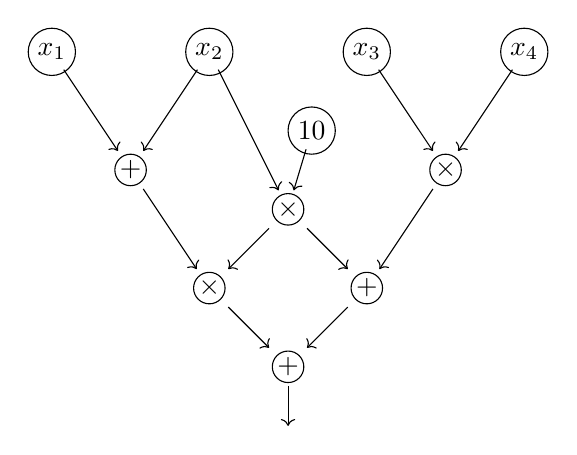
\begin{tikzpicture}
  % draw a grid starting at -4,-3 until 4,3
%  \draw[help lines] (-4,-3) grid (4, 3);

  \draw (-3, 3) circle [radius=0.3] node (x1) {$x_1$};
  \draw (-1, 3) circle [radius=0.3] node (x2) {$x_2$};
  \draw ( 1, 3) circle [radius=0.3] node (x3) {$x_3$};
  \draw ( 3, 3) circle [radius=0.3] node (x4) {$x_4$};
  \draw ( 0.3, 2) circle [radius=0.3] node (const1) {$10$};
  
  \draw ( -2, 1.5) circle [radius=0.2] node (add1) {$+$};
  \draw (  0, 1) circle [radius=0.2] node (mul1) {$\times$};
  \draw (  2, 1.5) circle [radius=0.2] node (mul2) {$\times$};

  \draw ( -1, 0) circle [radius=0.2] node (mul3) {$\times$};
  \draw (  1, 0) circle [radius=0.2] node (add2) {$+$};

  \draw (  0, -1) circle [radius=0.2] node (add3) {$+$};

  \draw[->] (x1) -- (add1);
  \draw[->] (x2) -- (add1);
  \draw[->] (x2) -- (mul1);
  \draw[->] (x3) -- (mul2);
  \draw[->] (x4) -- (mul2);
  \draw[->] (const1) -- (mul1);
  \draw[->] (add1) -- (mul3);
  \draw[->] (mul1) -- (mul3);
  \draw[->] (mul1) -- (add2);
  \draw[->] (mul2) -- (add2);
  \draw[->] (mul3) -- (add3);
  \draw[->] (add2) -- (add3);
  \draw[->] (add3) -- (0, -1.75);
\end{tikzpicture}

  \captionof{figure}[Example of an arithmetic circuit.]{
    Representation of the polynomial $f = 10x_2 (x_1 + x_2) + ((x_3 x_4)
    + 10x_2)$ as an arithmetic circuit.\label{fig:ac}
  }
\end{center}

%\section{Boolean vs Arithmetic}
Boolean circuits are not as highly structured as arithmetic circuits due to the
algebraic nature of of the latter.
That is why is is possible to prove results in the arithmetic world that are
still considered open in the Boolean world.
One very common problem related to circuits is to determine lower bounds i.e.,
prove that for a circuit computing $f$, there isn't any other better circuit.
For arithmetic circuits, there are super-linear bounds known on the size of the
circuit, while in the Boolean case, this is much harder to prove.

%\begin{definition}
%  A boolean circuit over the set of variables $X = \{\setSpace{x}{1}{n}\} \in
%  \{0, 1\}^n$ is a directed acyclic graph with the following properties.  The
%  nodes of the graph are called \emph{gates}. Every gate of in-degree (or
%  \emph{fan-in}) 0 is labeled by either a variable from $X$ or by a constant
%  $\{0, 1\}$. Gates with fan-in $k > 0$ are labeled by one of the boolean
%  functions $\AND$, $\OR$, $\NOT$ on on $k$ inputs, and in the case of $\NOT$,
%  $k = 1$. The gates with \emph{fan-out} 0 are \emph{output gates}.
%  \label{def:boolean}
%\end{definition}
%
%The notions of size and depth are exactly the same as the ones in arithmetic
%circuits.

It is worth noting that when using arithmetic circuits we are usually concerned
with polynomials of a particular form, which then fixes the set of computable
functions (i.e., polynomials in $\bbF[X]$). With Boolean circuits it is usually
the reverse, where we are interested in computing functions from $\bbF^{|X|}$
to $\bbF$.
%It is worth noting that when using boolean circuits the interest is not in any
%specific representation of the function but rather in just \emph{some}
%representation of it, while with arithmetic circuits the focus is on
%a \emph{specific} representation of the function or polynomial, i.e., we are
%concerned with polynomials a particular form, which then fixes the set of
%computable functions.
%In other words, with boolean circuits the interest is in the \emph{semantics}
%of the computation, while with arithmetic circuits the interest is on
%\emph{syntactic} computation of polynomials.
%Basically, with arithmetic circuits we usually are concerned with
%polynomials of a particular form, which then fixes the set of computable
%functions. With Boolean circuits it is usually the reverse.
%This is an important point when studying circuits because we are not interested
%in the formal computation of functions but rather in the functions that these
%circuits define.
%
In the arithmetic case, this is because a function may be expressed by
a polynomial in several ways, while, in general, a polynomial defines a unique
function. A simple example is the function $f = x^2 + x$, which defines the
zero polynomial, but only under $\bbF_2$.

%In the boolean case there is no interest in any specific polynomial
%representation of the function but rather in just \emph{some} representation of
%it, while in the arithmetic scenario the focus is on a \emph{specific}
%representation of the function. That is, with boolean circuits the interest is
%on the \emph{semantics} of the polynomial computation, while in arithmetic
%circuits the interest is on the \emph{syntactic} of the computation. This is
%important to be stressed out since we are not interested in the formal
%computation of polynomials rather than the functions that these polynomials
%define.
%It is important to stress that arithmetic circuits should be seen as computing
%\emph{specific} polynomials in $\bbF[X]$ rather than functions from
%$\bbF^{|X|}$ to $\bbF$. Essentially, one is interested in the formal
%computation of polynomials rather the functions that these polynomials define.

%When the field is $\bbF_2$ and every gate of the circuit as at most two inputs,
%the circuit is a \emph{boolean circuit}. While these circuits provide a nice
%mathematical model of a program inside a modern computer, they are not of much
%(practical) interest to us since they only handle the evaluation of binary
%functions. We will instead rely on the previously introduced arithmetic
%circuits where instead of using a binary field like in boolean circuits they
%use a field $\bbF_p$, for a given $p$\footnote{One can easily observe that an
%arithmetic circuit over $\bbF_2$ can be seen a boolean circuit}.

For arithmetic circuits, a natural question that may arise is: since there are
only $+$ and $\times$ gates, why not add a $\div$ gate to the set of allowed
operations? In the past this model was actually considered, but if we add
a $\div$ gate, this gate now computes a rational function instead of
a polynomial.  Also the problem of dividing by a zero polynomial arises, so
there needs to be a restriction for this case. But as it turns out, it is
possible to represent the division gate using only $+$ and $\times$ gates, with
some polynomially additional cost. These solutions were first introduced by
Strassen, and later by Hrube\u{s} and Yehudayof (see
\cite[Section~2.5]{Shpilka:2010} for details on both solutions and proof
sketches).

From now on we will only focus on arithmetic circuits, and so when using the
term circuit we are referring to an arithmetic circuit.

\section{Circuit Evaluation}\label{sec:circeval}
We already know how circuits are represented and what operations they compute.
But how do we efficiently evaluate them? This is critical for us because the
evaluation of a circuit shouldn't become too slow when comparing to a native
evaluation (i.e., evaluation a function on a Turing machine model). This is
even more critical as circuits start to grow, reaching sizes in the orders of
hundreds of inputs and thousands of gates.

If we look at the circuit representation, it is simply a \nom{DAG}{Directed
Acyclic Graph} that represents the dependencies between gates. That is, the
inputs of a gate $g$ are its dependencies, and therefore we cannot evaluate $g$
before we evaluate its inputs. So we can treat a circuit as a \emph{dependency
graph}. For such graphs it is possible to generate an \emph{evaluation order}
using some topological sort algorithm. Some of these algorithms perform checks
to detect whether the graph is cyclic or not, but for our case we always assume
that graphs are acyclic. These kind of algorithms are fundamental for many of
common computing applications such as program (re)compilation, system package
management or spreadsheet calculators.

The common algorithm used for topological sort is based on the
\nom{DFS}{Depth-First Search}~\cite{tarjan1972depth}, a depth search algorithm
over graphs. Basically, edges are explored out of the most recently visited
vertex $g$ that still has unexplored edges leaving it. When all of $g$'s edges
have been visited, the search ``backtracks'' to explore edges leaving the
vertex from which $g$ was explored. This process continues until all the
vertices that are reachable from the original source have been visited. If
a vertex is left unvisited, then it is used as a new source for the DFS and the
``backtracking'' process is repeated again. This process is repeated until all
vertices in the graph have been visited. The running time of DFS is $\Theta(V
+ E)$ with $V$ the number of vertices and $E$ the number of edges. A simple DFS
can be implemented as shown in \refalg{alg:dfs}.

\begin{algorithm}
  \begin{algorithmic}[1]
    \Function{DFS}{G}\Comment{Acyclic graph $G = (V,E)$}
      \For{each vertex $u \in V$}
        \State $u.color \gets$ WHITE
      \EndFor
      \State $time \gets 0$\Comment{Global variable to keep track of time}
      \For{each vertex $u \in V$}
        \If{$u.color$ == WHITE}
          \State \Call{DFS-Visit}{$G$, $u$}
        \EndIf
      \EndFor
    \EndFunction
    \Statex
    \Function{DFS-Visit}{$G,u$}
      \State $time \gets time + 1$
      \State $u.d \gets time$\Comment{Time at which white vertex $u$ was discovered}
      \State $u.color \gets$ GRAY
      \For{each vertex $v \in G.Adj[u]$}
        \If{$v.color$ == WHITE}
          \State \Call{DFS-Visit}{$G, v$}
        \EndIf
      \EndFor
      \State $u.color \gets$ BLACK\Comment{Vertex $u$ is finished}
      \State $time \gets time + 1$
      \State $u.f \gets time$\Comment{Time at which black vertex $u$ was
        finished}
    \EndFunction
  \end{algorithmic}
  \caption{Basic DFS.}
  \label{alg:dfs}
\end{algorithm}


By the end of DFS there are two timestamps in each vertex $u$: $u.d$ represents the
time at which it was first visited and $u.f$ represents the time at which all
of its children edges where visited. For each vertex $u$, it holds that
$u.d < u.f$ and their values are in $\{ 1, \dotsc, 2\abs{V} \}$.

%\begin{center}
%  \centering
%  %\input{Graphics/example-dfs}
%  \missingfigure{execute DFS on the example circuit}
%  \captionof{figure}[Depth First Search on a simple directed acyclic graph.]{
%    DFS of a DAG.\label{fig:dfs}
%  }
%\end{center}

A topological sort of a DAG $G = (V, E)$ is a linear ordering of all its
vertices such that if $G$ contains an edge $(u, v)$, then $u$ appears before
$v$ in the ordering. Any DAG has at least one topological ordering. Given an
arithmetic circuit, its topological sort can be viewed as an ordering of its
gates along a horizontal line so that all directed edges go from left to right.
%Considering the arithmetic circuit from \reffigure{fig:ac}, one of the possible
%topological orderings is:
%
%\begin{center}
%  \centering
%  %\input{Graphics/example-tsort}
%  \missingfigure{execute topo-sort on the example circuit}
%  \captionof{figure}[Topological sort of a simple directed acyclic graph.]{
%    Topological sort of a DAG.\label{fig:tsort}
%  }
%\end{center}

With DFS, a topological sorting becomes as simple as the following:
\begin{algorithm}
  \begin{algorithmic}[1]
    \Function{Topo-Sort}{$G$}
      \State \Call{DFS}{$G$}\Comment{To compute the finishing times $u.f$ for
      each vertex of $G$}
      \State Output a list $L$ in order of decreasing finishing times
    \EndFunction
  \end{algorithmic}
  \caption{A simple topological sorting algorithm, using DFS as in
    algorithm~\ref{alg:dfs}.}
  \label{alg:tsort}
\end{algorithm}


Since DFS takes time $\Theta(V + E)$ and the insertions on the list $L$ take
time $\calO(1)$, the total running time of a topological sorting based on a DFS
is $\Theta(V + E)$.

Finally, to perform the circuit evaluation we simply evaluate each gate in the
order defined by the list $L$ obtained with \textsc{Topo-Sort}. Each gate
evaluation result is kept on a list, where the last index corresponds to the
circuit's output gate.

We will be using \citetool{parno:howell:gentry:raykova:2013} to generate
circuits, and in that case, there is practically no advantage in using
a topological sorting algorithm to perform the evaluation because most of the
the circuits from \citetool{parno:howell:gentry:raykova:2013} are already
properly sorted. However, if using custom designed circuits or circuits
generated by some other means, it is necessary to generate a topological
ordering to be able to efficiently evaluate the circuit.

The reason why we are solely interested in arithmetic circuits is because they
allows to represent computations as multivariate polynomials that can be
efficiently computed. This is very important specially for our homomorphic
scenario.

\section{Circuit generation}
Even though arithmetic circuits are quite clean and simple in theory, there are
not many tools to easily compile a piece of code into a circuit representation.
At this moment, the ones from \textcite{parno:howell:gentry:raykova:2013}
(\citetool{parno:howell:gentry:raykova:2013}) and from \textcite{tinyram}
(\citetool{tinyram}) are the most efficient.

\textcite{tinyram} functionality is clearly superior because it is essentially
a port of the gcc\footnotemark compiler. Basically, \citetool{tinyram} takes
a \texttt{C} program and compiles it to a specific \citetool{tinyram} assembly
language, which is equivalent to an arithmetic circuit. Unfortunately, we
cannot easily access the arithmetic circuit but only its binary representation.
\footnotetext{\url{https://gcc.gnu.org/}}

%At this moment, the most complete and with support for more operations is the
%one of \textcite{parno:howell:gentry:raykova:2013}
%(\citetool{parno:howell:gentry:raykova:2013}).

On the other hand, \citetool{parno:howell:gentry:raykova:2013} comes equipped
with a compiler that converts a subset of the \texttt{C} language and outputs
an arithmetic circuit representation, and this is the reason why we are using
it instead of \citetool{tinyram}.
They have support for both boolean and arithmetic circuit generation, but as it
was previously mentioned, we are only interested on arithmetic circuits. They
also mention that the use of boolean circuits as opposed to arithmetic circuits
proved to be much slower, specially on their setting of verifiable computation.

The compiler, written in Python, can process a substantial subset of
\texttt{C}: global, function and block-scoped variables; arrays, struct's and
pointers; function calls, conditional loops; static initializers; arithmetic
and bit-wise operators; and pre-processor directives. The piece of code that we
wish to convert to a circuit must be inside the function \texttt{void
outsource(struct Input *, struct Output *)}. The parameters describe the input
and output values, respectively.

Because circuits only supports expressions and not mutable state and
iteration, the \texttt{C} program's semantics is restricted. There is no
support for dynamic operations (like memory allocations), and everything must
be compile-time constant (as pointers or array dereferences).

Their notion of arithmetic circuits is complemented with one more gate
operation: a \emph{split gate}. Basically, given a value $a \in \bbF_p$ where
$p$ is an integer with $k$ bits, the split gate outputs to $k$ gates, where
each of them represents the bit value $a_i$. Given such
binary values, it is possible to compute Boolean functions using only
arithmetic gates: $\mathrm{NAND}(a,b) = 1 - ab$, $\mathrm{AND}(a,b) = ab$,
$\mathrm{OR}(a,b) = 1 - (1 - a)(1 - b)$; each of these operations comes at the
cost of only one multiplication.

The recombination of the $k$ bits into a single gate is given by the expression
$\sum_{i=1}^{k}{2^{i - 1}a_i}$. As they noticed, recombining these $k$ bits
into an integer is not very costly as they only perform additions and
multiplications by constants, which are practically free.

In the setting of VC and SNARKs\footnotemark, the interest is in the
verification of computations rather than efficiently compute them
homomorphically (which is our case). That is why they introduced a split gate,
which is very efficiently verifiable and allows them to compute more
operations.  \footnotetext{\citetool{parno:howell:gentry:raykova:2013} and
\citetool{tinyram} were constructed with VC and SNARKs in mind.}

\section{Limitations}
One problem with circuit generation has to do with \emph{data dependencies}.
While the circuit's inputs do not affect its topology, they affect the program
flow and memory accesses. Thus, a circuit must be ready to support a wide range
of program flows and memory accesses, despite the fact that its topology has
already been set. The technique \citetool{parno:howell:gentry:raykova:2013}
uses to generate circuits is \emph{program analysis}.
With program analysis, if the program and its inputs are known in advance,
generating the corresponding circuit is simple: build the circuit's topology to
match the pre-determined program flow and its memory accesses. But if only the
program is known in advance, and not its inputs, the program must be analyzed
piece by piece (i.e., unroll loops, branches, etc) so that the circuit can
handle different input values. However, this technique has one big limitation.
The class of supported programs is not very broad, as
\citetool{parno:howell:gentry:raykova:2013} requires arrays accesses and loop
iterations bounds to be compile-time constants, which forces us to ``write
around'' this limited functionality.

Unfortunately, the introduction of the split gate is a limitation for us
because we are not solely interested in an efficient verification (as with VC
and SNARKs), which it limits even more the subset of \texttt{C} code that we
can convert to arithmetic circuits. This means that we cannot have conditional
dependencies which means that everything must be known at compile time (except
for the input values), and we cannot also use any bit-wise operation since they
give origin to split gates.

However, we can still write simple \texttt{C} programs and use
\citetool{parno:howell:gentry:raykova:2013} to convert them to arithmetic
circuits, so that they can be used by the \citescheme{catalano:fiore:2013}
scheme.

 % Circuits

\chapter{Homomorphic Authenticators}\label{chap:homo-auth}

A trivial solution to the problem of enforcing authenticity of outsourced
computations would be to make the server send the entire data and the computed
signatures/MACs (we will refer to both of them as tags from now on) back to the
client, and then she would compute the function herself and compare the
results. But by using homomorphic authentication primitives, and by sending
only the tags and the output of the function back to the client, beyond saving
bandwidth, the amount of information revealed to the client about the data set
is much smaller. Also, this trivial solution does not guarantee efficiency
which is one of the requirements to enforce the authenticity of computations.

% Remove this paragraph if using the Definitions section
Let us now introduce some basic notions and definitions necessary to build
homomorphic authentication schemes, as well as some constructions. From now on,
it is always assumed that Alice stores the data and tags on some possibly
untrusted server.

%% ---------------------------------------------------------------------------
% HOMOMORPHIC SIGNATURES
%% ---------------------------------------------------------------------------
\section{Homomorphic Signatures}\label{sec:def-hsig}
A homomorphic signature scheme allows the computation of functions on
previously signed data to obtain a derived signature, and later anyone with the
public key can verify the results.  This is known as \emph{public
verifiability}. The computed signature authenticates both the function and the
result of applying the function to the data.

In the only construction presented so far (beyond linear),
\textcite{boneh:freeman:2011} complemented the definition of homomorphic
signatures first introduced by \textcite{johnson:molnar:song:wagner:2002}.
Basically, Alice has a (numerical) data set $\mSpace{1}{n}$, and she signs each
message $m_i$, but before signing she augments it with a label $\tau$ and an
index $i$.  For each message, she signs $(\tau, m_i, i)$ and obtains $n$
independent signatures $\vec{\sigma} = \sigmaSpace{1}{n}$. The value of the
label $\tau$ serves as a name to the data set and binds its members together.

Later, one can ask the server to compute functions on some portion of the data.
To compute a function $f$, the server uses a public key homomorphic evaluation
algorithm that basically signs the triple $(\tau, m := f(\mSpace{1}{n}),
\langle f\rangle)$, where $\langle f\rangle$ is an encoding of the function
$f$.
%
This evaluation algorithm only acts on signatures, not in the original
messages. The pair $(m, \sigma)$ can be made public and anyone can check that
the server correctly computed $f$ over the data set by verifying that $\sigma$
is a signature on triple $(\tau, m, \langle f\rangle)$.  The derived signature
$\sigma$ authenticates both the function $f$ and the result of computing $f$
over the data. Using the pair $(m, \sigma)$, one can derive signatures on
functions of $m$ and other signed data.  The short label $\tau$ is used to
prevent mixing of data from different data sets when evaluating functions.

Like ``regular'' signature schemes, a homomorphic signature scheme consists of
the usual algorithms \KeyGen, \Sign and \Vrfy as well as an additional \Eval
that evaluates a given function on a set of previously signed messages. If
$\vec{\sigma}$ is a valid set of signatures authenticating messages $\vec{m}$,
then $\Eval(f,\vec{\sigma})$ should be a valid signature for $f(\vec{m})$.  It
is worth noting once again that \Eval only acts on already signed messages.
\begin{definition}
  A \emph{homomorphic signature scheme} $\HSIG$ is a tuple of
  \nom{PPT}{Probabilistic-Polynomial Time} algorithms (\KeyGen, \Sign, \Vrfy,
  \Eval) as follows:
  \begin{description}
    \item[$\KeyGen(1^\lambda, n) \to (\pk,\sk)$:] Takes a security
      parameter $\lambda$ and a maximum data set size $n$. Outputs a public and
      secret key, \pk and \sk, respectively.  The public key also defines
      a message space $\calM$, a signature space $\Sigma$ and a set $\calF$ of
      all ``admissible'' functions $\function{f}{\calM^n}{\calM}$.
    \item[$\Sign_\sk(\tau, m, i) \to \sigma$:] Receives a label $\tau
      \in \{0,1\}^\lambda$, a message $m \in \calM$ and an index $i \in \{1,
      \dotsc, n\}$, and outputs a signature $\sigma \in \Sigma$.
    \item[$\Vrfy_\pk(\tau, m, \sigma, f) \to
      \{\mathsf{accept,reject}\}$:] Receives a label $\tau \in \{0,
      1\}^\lambda$, a message $m \in \calM$, a signature $\sigma \in \Sigma$,
      a function $f \in \calF$, and outputs either \textsf{accept} or
      \textsf{reject}.
    \item[$\Eval_\pk(\tau, f, \vec{\sigma}) \to \sigma'$:] Receives
      a label $\tau \in \{0,1\}^\lambda$, a function $f \in \calF$, a tuple of
      signatures $\vec{\sigma} \in \Sigma^n$, and outputs a signature $\sigma'
      \in \Sigma$.
  \end{description}
\end{definition}

A signature scheme like the one presented above is said to be
\emph{$\calF$-homomorphic}, or \emph{homomorphic with respect to $\calF$}.

Let $\function{\pi_i}{\calM^n}{\calM}$ be the function that projects onto the
$i$th element, i.e., $\pi_i(\mSpace{1}{n}) = m_i$. It is required that for all
\pk generated by \KeyGen, $\setSpace{\pi}{1}{n} \in \calF$. A homomorphic
signature scheme must achieve the following properties: authentication and
evaluation correctness, unforgeability and length efficiency.

\paragraph*{Authentication correctness}For each $(\pk, \sk)$, all labels $\tau
\in \{0,1\}^\lambda$, all $m \in \calM$, and all $i \in \{\interval{1}{n}\}$,
if $\sigma \gets \Sign_\sk(\tau, m, i)$, then it holds:
\begin{equation}\label{eq:hsig-auth-corr}
  \Pr[\Vrfy_\pk(\tau, m, \sigma, \pi_i) = \mathsf{accept}] \geq
  1 - \negl(\lambda).
\end{equation}

\paragraph*{Evaluation correctness} For each $(\pk, \sk)$, all $\tau \in
\{0,1\}^\lambda$, all tuples $\vec{m} = (\mSpace{1}{n}) \in \calM^n$, and all
functions $f \in \calF$, if $\sigma_i \gets \Sign_\sk(\tau, m_i, i)$ for $i
= \interval{1}{n}$ and $\sigma' = \Eval_\pk(\tau, f, (\sigmaSpace{1}{n}))$ it
must hold:
\begin{equation}\label{eq:hsig-eval-corr}
  \Pr[\Vrfy_\pk(\tau, f(\vec{m}), \sigma', f) = \mathsf{accept}] \geq
  1 -\negl(\lambda).
\end{equation}

The \Eval algorithm can take as input derived signatures produced by \Eval
itself, but doing so for a large number of iterations may eventually reach
a point where the input signatures are valid, but the output signature is not.
For this reason, and to simplify, the evaluation correctness property is
limited so that it only requires that \Eval produces a valid output when given
as input only signatures produced by the \Sign algorithm.

\paragraph*{Unforgeability} Informally, a forgery under a chosen message attack
is a valid signature $\sigma$ on a triple $(\tau, m, f)$ such that $m \neq
f(\mSpace{1}{n})$ where $\mSpace{1}{n}$ is the data set signed using label
$\tau$.

\begin{definition}
  A homomorphic signature scheme $\HSIG = (\KeyGen, \Sign, \Vrfy, \Eval)$ is
  \emph{unforgeable} if for all $n$ the advantage of any PPT adversary $\calA$ in
  the following game is negligible in the security parameter $\lambda$:
  \begin{description}
    \item[Setup:] The challenger obtains $(\pk, \sk) \gets_\$
      \KeyGen(1^\lambda, n)$ and gives \pk to $\calA$.  \pk defines a message
      space $\calM$, a signature space $\Sigma$, and a set $\calF$ of admissible
      functions $\function{f}{\calM^n}{\calM}$.
    \item[Queries:] Proceeding adaptively, $\calA$ specifies a sequence of data
      sets $\vec{m}_i \in \calM^n$. For each $i$, the challenger chooses label
      $\tau_i$ uniformly from $\{0, 1\}^\lambda$ and gives to $\calA$ the label
      $\tau_i$ and the signatures $\sigma_{ij} \gets \Sign_\sk(\tau_i,
      m_{ij}, j)$ for $j = \interval{1}{n}$.
    \item[Output:] $\calA$ outputs a label $\tau^* \in \{0, 1\}^\lambda$,
      a message $m^* \in \calM$, a function $f \in \calF$, and a signature
      $\sigma^* \in \Sigma$.
  \end{description}
\end{definition}

The adversary $\calA$ wins if $\Vrfy_\pk(\tau^*, m^*, \sigma^*, f)
= \mathsf{accept}$ and either:
\begin{itemize}
  \item \emph{Type I forgery}: $\tau^* \neq \tau_i$ for all $i$, or
  \item \emph{Type II forgery}: $\tau^* = \tau_i$ for some $i$, but $m^* \neq
    f(\vec{m}_i)$.
\end{itemize}

The advantage of $\calA$ is the probability that $\calA$ wins the game.

\paragraph*{Privacy} In this setting, privacy means that given signatures on
a data set $\vec{m} \in \calM^n$, the derived signatures on messages
$\functionSpace{f}{1}{s}{\vec{m}}$ do not leak any information about $\vec{m}$
beyond what is revealed by computing the functions $\fSpace{1}{s}$ known to the
attacker over the data set $\vec{m}$. While the original data set $\vec{m}$ is
kept hidden, the fact that a derivation took place is not. The verifier should
be able to verify that the correct function was applied to the original data.

More precisely, privacy is ensured using \emph{weakly context hiding}. This
means that given signatures on a number of messages derived from two different
data sets, the attacker cannot tell from which data set the derived signatures
came from, and furthermore that this holds when the secret key is leaked. The
reason to be called ``weak'' is that the original signatures on the data are
not public.

\begin{definition}\label{def:hsig-priv}
  A homomorphic signature scheme $\HSIG = (\KeyGen, \Sign, \Vrfy, \Eval)$ is
  \emph{weakly context hiding} if for all $n$, the advantage of any PPT
  adversary $\calA$ in the following game is negligible in the security
  parameter $\lambda$:
  \begin{description}
    \item[Setup:] The challenger invokes \KeyGen to generate $(\pk,\sk)$, and
      gives the pair to $\calA$. \pk defines a message space $\calM$, a signature
      space $\Sigma$, and a set $\calF$ of admissible functions
      $\function{f}{\calM^n}{\calM}$
    \item[Challenge:] $\calA$ outputs $(\vec{m}_0^*, \vec{m}_1^*,
      \fSpace{1}{s})$
      with $\vec{m}_0^*, \vec{m}_1^* \in \calM^n$ and $\fSpace{1}{s} \in \calF$.
      For all $i = \interval{1}{s}$ it satisfies that $f_i(\vec{m}_0^*)
      = f_i(\vec{m}_1^*)$. These functions can be output adaptively after
      $\vec{m}_0^*, \vec{m}_1^*$ are output.

      Then the challenger generates a random bit $b \in \{0, 1\}$ and a random
      label $\tau \in \{0, 1\}^\lambda$. It signs the messages in $\vec{m}_b$
      using the label $\tau$ to obtain a vector $\vec{\sigma}$ of $n$ signatures.
      
      Next, for $i = \interval{1}{s}$ the challenger computes a signature
      $\sigma_i = \Eval_\sk(\tau, f_i, \vec{\sigma})$.
      
      It sends to $\calA$ the label $\tau$ and the signatures
      $\sigmaSpace{1}{s}$.
  \item[Output:] $\calA$ outputs a bit $b'$.

      $\calA$ wins the game if $b = b'$. The advantage of $\calA$ is the
      probability that $\calA$ wins the game.
  \end{description}
\end{definition}

If an attacker wins the previous game, it means that she can determine if the
challenge signatures were derived from $\vec{m}_0^*$ or $\vec{m}_1^*$.
A signature scheme is \emph{$s$-weakly context hiding} if the attacker cannot
win the game after seeing at most $s$ signatures derived from two different
data sets.

\paragraph*{Length efficiency}Informally, a signature scheme is length
efficient if for a fixed security parameter $\lambda$, the length of the
derived signatures depends only logarithmically on the size $n$ of the data
set.
% Not sure if succintness is the same as length efficiency. Succinctness is
% usually a property of proofs. But it seems analogous.

\begin{definition}
  A homomorphic scheme $\HSIG = (\KeyGen, \Sign, \Vrfy, \Eval)$ is \emph{length
  efficient} if there is some function $\function{\mu}{\bbN}{\bbR}$ such that
  for all $(\pk,\sk)$ obtained with \KeyGen, all $\vec{m} = (\mSpace{1}{n}) \in
  \calM^n$, all labels $\tau \in \{0, 1\}^\lambda$, and all functions $f \in
  \calF$, if
  \begin{equation}\label{eq:hsig-len-eff1}
    \sigma_i \gets \Sign_\sk(\tau, m_i, i) \quad \text{for all }i
    = \interval{1}{n}
    %\forall i \in \{0, \dotsc, n\}, \quad \sigma_i \gets
    %\Sign_\sk(\tau, m_i, i), 
  \end{equation}
  then for all $n > 0$ and for a derived signature $\sigma
  = \Eval_\pk(\tau, f, (\sigmaSpace{1}{n}))$, it holds:
  \begin{equation}\label{eq:hsig-len-eff2}
    \Pr[\len(\sigma) \leq \mu(\lambda) \cdot \log{n}] \geq 1 - \negl(\lambda).
  \end{equation}
\end{definition}

%% ---------------------------------------------------------------------------
% BONEH-FREEMAN CONSTRUCTION
%% ---------------------------------------------------------------------------
\subsection{Boneh-Freeman}\label{subsec:bf}
\citescheme{boneh:freeman:2011} is the first homomorphic signature scheme that
is capable of evaluating multivariate polynomials of bounded degree. All
previous schemes focused solely on \emph{linear functions}, while their scheme
allows the computation of various statistical functions like mean or standard
deviation.
%
They also proposed an improved linear scheme with support for linear functions
for small fields $\bbF_p$, specially for $p = 2$.

Here we will present an overview of their two constructions. A more detailed
description can be found in~\cite{boneh:freeman:2011}, as well as suitable
parameters and sampling algorithms necessary for the full definition of the
scheme. Both constructions rely on lattice-based techniques. They are build on
the ``hash-and-sign'' signatures of
\textcite{gentry:peikert:vaikuntanathan:2008}.

Abstractly, in~\citescheme{gentry:peikert:vaikuntanathan:2008}, the public key
is a lattice $\Lambda \subset \bbZ^\lambda$ and the secret key is a short basis
of $\Lambda$. To sign a message $m$, the holder of the secret key hashes $m$ to
an element $H(m) \in \bbZ^\lambda/\Lambda$ and samples a short vector $\sigma$
from the coset of $\Lambda$ defined by $H(m)$. The verification of $\sigma$ is
simply checking that $\sigma$ is short and that $\sigma \bmod{\Lambda} = H(m)$.

\subsubsection*{Linearly homomorphic scheme}
In a (linearly) homomorphic signature scheme, the message space is defined as
$\bbF^\lambda_p$ and a function
$\function{f}{(\bbF^\lambda_p)^n}{\bbF^\lambda_p}$ is encoded as
$f(\mSpace{1}{n}) = \sum_{i = 1}^{n}c_i m_i$. The $c_i$ are integers in $(-p/2,
p/2]$ and the description of $f$ is  $\langle f \rangle := (c_1, \dotsc, c_n)
\in \bbZ^n$.
%
To authenticate both the message and the function, as well as binding them
together, a single \citescheme{gentry:peikert:vaikuntanathan:2008} signature is
computed that is simultaneously a signature on the (unhashed) message $m \in
\bbF^\lambda_p$ and a signature on the hash of $\langle f \rangle$.

Such signature is obtained by using the ``intersection method''.
\textcite{boneh:freeman:2011} described it as follows. Let $\Lambda_1$ and
$\Lambda_2$ be $\lambda$-dimensional integer lattices with $\Lambda_1
+ \Lambda_2 = \bbZ^\lambda$. Suppose $m \in \bbZ^\lambda/\Lambda_1$ is
a message and $\function{\omega_\tau}{\bbZ^n}{\bbZ^\lambda/\Lambda_2}$ is
a hash function, dependent of $\tau$, that maps encodings of functions $f$ to
elements of $\bbZ^\lambda/\Lambda_2$.
%
Since $m$ defines a coset of $\Lambda_1$ in $\bbZ^\lambda$ and $\omega_\tau$
defines a coset of $\Lambda_2$ in $\bbZ^\lambda$, by the \nom{CRT}{Chinese
Remainder Theorem} the pair $(m, \omega_\tau(\langle f \rangle))$ defines
a unique coset of $\Lambda_1 \cap \Lambda_2$ in $\bbZ^\lambda$. Then, a short
vector $\sigma$ is computed with the property that $\sigma
= m \bmod{\Lambda_1}$ and $\sigma = \omega_\tau(\langle f \rangle)
\bmod{\Lambda_2}$. The vector $\sigma$ is a signature on $(\tau, m, \langle
f \rangle)$ that ``binds'' $m$ and $\omega_\tau(\langle f \rangle)$ -- an
attacker cannot generate a new short vector $\sigma'$ from $\sigma$ such that
$\sigma = \sigma' \bmod{\Lambda_1}$ but $\sigma \neq \sigma' \bmod{\Lambda_2}$.

In this linear scheme, $\bbF^\lambda_p \cong \bbZ^\lambda/\Lambda_1$ with the
isomorphism given explicitly by the map $\vec{\mathrm{x}} \mapsto
(\vec{\mathrm{x}} \bmod{\Lambda_1})$, and $\bbF^\ell_q \cong
\bbZ^\lambda/\Lambda_2$.

Using the above method, $\Sign_\sk(\tau, m, i)$ generates a signature on
$(\tau, m, \langle \pi_i \rangle)$, where $\pi_i$ is the $i$th \emph{projection
function} defined by $\pi_i(\mSpace{1}{n}) = m_i$ and encoded by $\langle \pi_i
\rangle = \vec{\mathrm{e}}_i$, the $i$th unit vector in $\bbZ^n$.

To authenticate the linear combination $m = \sum_{i = 1}^{n}c_i m_i$ previously
authenticated, compute the signature $\sigma := \sum_{i = 1}^{n}c_i \sigma_i$.
If $n$ and $p$ are sufficiently small, then $\sigma$ is a short vector. The
following homomorphic property is achieved:
\begin{align}
  \sigma \bmod{\Lambda_1} &= \sum_{i = 1}^n c_i m_i = m, \text{and} \nonumber \\
  \sigma \bmod{\Lambda_2} &= \sum_{i = 1}^n c_i \omega_\tau(\langle \pi_i
  \rangle) = \sum_{i=1}^{n}c_i \omega_\tau(\vec{\mathrm{e}}_i).
  \label{eq:bf-lin-homo-prop}
\end{align}

If $\omega_\tau$ is linearly homomorphic then $\sum_{i = 1}^n c_i
\omega_\tau(\vec{\mathrm{e}}_i) = \omega_\tau\left( (c_1, \dotsc, c_n \right))$
for all $c_i \in \bbZ$. Since $(c_1, \dotsc, c_n)$ is exactly the encoding
$\langle f \rangle$, the signature $\sigma$ authenticates both the message $m$
and the fact that $m$ is indeed the output of $f$ applied to the original
messages $m_1, \dotsc, m_n$.

Verification of a signature $\sigma$ is simply checking that
\begin{align}
  \sigma \bmod{\Lambda_1} & \equals m, \nonumber \\
  \sigma \bmod{\Lambda_2} & \equals \omega_\tau(\langle f \rangle).
  \label{eq:bf-lin-vrfy}
\end{align}

\paragraph*{Correctness} The above linearly homomorphic scheme satisfies both
authentication and evaluation correctness. The proofs can be found
in~\cite{boneh:freeman:2011}.

\paragraph*{Unforgeability} The security is based on the \nomsf{SIS}{Small
Integer Solution} problem on $q$-ary lattices for some prime $q$. More
precisely, for security parameter $\lambda$ it follows:
\begin{theorem}\label{theo:bf-lin-uf}
  If $\mathsf{SIS}_{q, \lambda, \beta}$ is infeasible for a suitable $\beta$,
  then the above linearly homomorphic scheme is unforgeable in the random
  oracle model.
\end{theorem}

To prove it, it is shown that a successful forger can be used to solve the
\textsf{SIS} problem in the lattice $\Lambda_2$, which for random $q$-ary
lattices (and suitable parameters) is as hard as standard worst case lattice
problems. The full proof and the suitable parameters can be found
in~\cite{boneh:freeman:2011}.

\paragraph*{Privacy} The above linearly homomorphic signature scheme is weakly
context hiding. Based on the fact that the distribution of a linear combination
of samples from a discrete Gaussian is itself a discrete Gaussian, it is proved
that a derived signature on a linear combination $m' = \sum_{i = 1}^{n} c_i
m_i$ depends (up to negligible distance) only on $m'$ and the $c_i$, and not on
the original messages $m_i$. The full proof can be found
in~\cite{boneh:freeman:2011}.

\paragraph*{Length efficiency} The bit length of a derived signature only
depends logarithmically on the size of the data set. The proof, along with the
exact length of a derived signature, can be found in~\cite{boneh:freeman:2011}.

\subsubsection*{Polynomially homomorphic scheme}
The basic idea for this scheme is as follows: what if $\bbZ^\lambda$ has a ring
structure and lattices $\Lambda_1, \Lambda_2$ are ideals? Then the maps
$\vec{\mathrm{x}} \mapsto \vec{\mathrm{x}} \bmod{\Lambda_i}$ are ring
homomorphisms, and therefore adding or multiplying signatures corresponds to
adding or multiplying the corresponding messages or functions. Since any
polynomial can be computed by repeated additions and multiplications, by adding
this structure to the previous scheme it is possible to authenticate polynomial
functions on messages.

Let $F(x) \in \bbZ[x]$ be a monic, irreducible polynomial of degree $\lambda$
and let $R$ be the ring $\bbZ[x]/(F(x))$. $R$ is isomorphic to $\bbZ^\lambda$
and ideals in $R$ correspond to integer lattices in $\bbZ^\lambda$ under the
``coefficient embedding''. This embedding maps a polynomial in $R$ to an
element in an ideal lattice as follows: if $g(x) = g_0 + g_1 x + \cdots
+ g_{\lambda-1} x^{\lambda - 1}$, then coefficient embedding can be defined as:
$g(x) \mapsto (g_0, \dotsc, g_{\lambda-1}) \in \bbZ^\lambda$.

$\Lambda_1$ and $\Lambda_2$ are specially chosen to be degree one prime ideals
$\mathfrak{p,q} \subset R$ of norm $p, q$ respectively, with $\mathfrak{p}
= (p, x - a), \mathfrak{q} = (q, x - b)$. $R/\mathfrak{p}$ and $R/\mathfrak{q}$
are isomorphic with $\bbF_p$ and $\bbF_q$, respectively. The message space is
defined by $\bbF_p$. \Sign is now exactly as in the linearly homomorphic
scheme, and it returns a short signature $\sigma \in R$.

When considering polynomial functions on $\bbF_p[x_1, \dotsc, x_n]$, the
projection functions $\pi_i$ are exactly the linear monomials $x_i$, and any
polynomial function can be obtained by adding and multiplying monomials.  If an
ordering on all monomials of the form $x_1^{e_1} \cdots x_n^{e_n}$ is fixed,
then it is possible to encode any polynomial function as its vector of
coefficients, with the $i$-th unit vector $\vec{\mathrm{e}}_i$ representing the
linear monomials $x_i$ for $i = 1, \dotsc, n$.

The hash function $\omega_\tau$ is defined exactly as in the linear scheme: for
a function $f$ in $\bbF_p[x_1, \dotsc, x_n]$ encoded as $\langle f \rangle
= (c_1, \dotsc, c_\ell) \in \bbZ^\ell$, define a polynomial $\hat{f} \in
\bbZ[x_1, \dotsc, x_n]$ that reduces to $f \bmod{p}$. Then,
$\omega_\tau(\langle f \rangle) = \hat{f}(\alpha_1, \dotsc, \alpha_n)$ where
each $\alpha_i \in \bbF_q$ is the output of the hash function $H(\tau || i)$.

The evaluation algorithm uses the lifting of $f$ to $\hat{f}$.  Given $f$ and
the signatures $\sigmaSpace{1}{n} \in R$ on messages $m_1, \dotsc, m_n \in
\bbF_p$, the signature on $f(m_1, \dotsc, m_n)$ is given by
$\hat{f}(\sigmaSpace{1}{n})$.
%
It returns a short signature $\sigma \in R$ on triple $(\tau, m, \langle
f \rangle)$ such that $\sigma = m \bmod{\mathfrak{p}}$ and $\sigma
= \omega_\tau(\langle f \rangle) \bmod{\mathfrak{q}}$. Let $\sigma_i$ be
a signature on $(\tau, m_i, \langle f_i \rangle)$ for $i = 1, 2$. The following
homomorphic properties can be observed:
\begin{align}
  \sigma_1 + \sigma_2 & \text{ is a signature on } (\tau, m_1+m_2, \langle f_1
  + f_2 \rangle) \nonumber \\
  \sigma_1 \cdot \sigma_2 & \text{ is a signature on } (\tau, m_1 \cdot m_2, \langle f_1
  \cdot f_2 \rangle)
  \label{eq:bf-poly-homo-prop}
\end{align}

The verification is essentially the same as in the linearly homomorphic scheme.

\paragraph*{Correctness} The above scheme satisfies both authentication and
evaluation correctness properties. Proof can be found
in~\cite{boneh:freeman:2011}.

\paragraph*{Unforgeability} To prove that the above scheme is unforgeable, it
is shown that a successful forger can be used to find a solution to the
\nom{SIVP}{Shortest Independent Vectors Problem} in the lattice $\Lambda_2$,
which in this scheme is the ideal $\mathfrak{q}$.

\paragraph*{Privacy} For large $p$, this homomorphic scheme is not weakly
context hiding as defined in \refdef{def:hsig-priv}.
In~\cite{boneh:freeman:2011} is is shown exactly why the signature $\sigma$
leaks information about the original messages $m_0, m_1$.

\paragraph*{Length efficiency} The bit length of a derived signature only
depends logarithmically on the size of the data set, for polynomials of bounded
constant degree and for small coefficients. The proof, along with the exact
length of a derived signature, can be found in~\cite{boneh:freeman:2011}.



%% ---------------------------------------------------------------------------
% HOMOMORPHIC MACS
%% ---------------------------------------------------------------------------
\section{Homomorphic MACs}\label{subsec:def-hmac}
The symmetric analogue of homomorphic signatures are homomorphic MACs.
%
Basically, Alice has a secret key which is used to generate a tag $\sigma$ that
authenticates a message $m$ under label $\tau$. Given a labeled program $\calP
= (f, \tauSpace{1}{n})$ and a set of tags $\sigmaSpace{1}{n}$, anyone can
execute the homomorphic evaluation algorithm over $\calP(\sigmaSpace{1}{n})$ to
generate a short tag $\sigma'$ that authenticates $m' = \calP(\mSpace{1}{n})$
as the output of the $\calP$ executed over inputs labeled by $\tauSpace{1}{n}$,
respectively.

There are three main properties that a homomorphic MAC scheme is required to
satisfy.%
\begin{inparaenum}[(1)]
\item It must be \emph{secure}, i.e., an adversary that asks for tags
  authenticating some messages of his own choice should not be able to produce
  valid tags authenticating messages that are not obtained as the output of
  $\calP$.
\item It should be \emph{succinct}, i.e., the output of $\calP$ can be
  certified using much less communication that than of sending the original
  authenticated messages.
\item Lastly, it should be \emph{composable} meaning that tags authenticating
  previous outputs of $\calP$ should be usable as inputs to further
  authenticate new computations, i.e., the tag authenticating the output of
  $\calP$ can be used as one of the inputs of another labeled program $\calP'$.
\end{inparaenum}

However, unlike in homomorphic signatures, it is necessary to explain what it
really means to authenticate a message as the output of a labeled program.
%
In a scenario where many users share the secret key and authenticate various
data-items without keeping any local or joint state, it is necessary to specify
which data is being authenticated and which data the program $\calP$ should be
evaluated on.
%
With this in mind, \textcite{gennaro:wichs:2012} defined the concept of
\emph{labeled programs}\footnote{\citeauthor{gennaro:wichs:2012} defined
labeled programs for boolean circuits $\function{f}{\{0, 1\}^n}{\{0,1\}}$, but
here we will consider the case for arithmetic circuits
$\function{f}{\bbF^n}{\bbF}$ where $\bbF$ is some finite field, like $\bbZ_p$
for some prime $p$.}.

\paragraph*{Labeled Programs} \emph{Labels} are used to index some data.
A labeled program $\calP = (f, \tauSpace{1}{n})$ consists of
a circuit\footnote{Or function.} $\function{f}{\bbF^n}{\bbF}$  and a distinct
input label $\tau_i \in \{0,1\}^\lambda$ for each input wire $i \in
\{\interval{1}{n}\}$ of the circuit. This can be seen as way to give useful
names to the variables of a program, without knowing the input values -- as an
example, we can consider a program that outputs the average salaries of
a company, and each $\tau_i$ can be of the form ``salary of worker $i$''.
%
A message $m$ is then authenticated with respect to a label $\tau$, and the
value of the label does not need to have any meaningful semantics. This
label-message association basically means that the value $m$ can be assigned to
those input variables of a labeled program $\calP$ whose label is $\tau$.
However, with this definition, a label \emph{cannot} be re-used for multiple
messages, i.e., two distinct messages $m, m'$ cannot be authenticated with
respect to the same label $\tau$. 

Given some labeled programs $\setSpace{\calP}{1}{t}$ and a circuit
$\function{g}{\bbF^t}{\bbF}$, the \emph{composed program} $\calP^*
= g(\setSpace{\calP}{1}{t})$ consists in evaluating a circuit $g$ on the
outputs of $\setSpace{\calP}{1}{t}$. The labeled inputs of the composed program
$\calP^*$ are just all the \emph{distinct} labeled inputs of
$\setSpace{\calP}{1}{t}$, and all the input wires with the same label are put
together in a single input wire.  The \emph{identity program} with label $\tau$
is denoted by $\calI_\tau := (g_{\id}, \tau)$, where $g_{\id}$ is the
\emph{canonical identity circuit} and $\tau \in \{0, 1\}^\lambda$ is some input
label. Any program $\calP = (f, \tauSpace{1}{n})$ can be written as
a composition of programs $\calP = f (\setSpace{\calI}{\tau_1}{\tau_n})$.

Given a labeled program $\calP = (f, \tauSpace{1}{n})$ and a set of tags
$\sigmaSpace{1}{n}$ that authenticates messages $m_i$ under label $\tau_i$
, anyone can run the homomorphic evaluation algorithm that takes an input the
tuple $(\calP, \sigmaSpace{1}{n})$ and whose output $\sigma'$ will authenticate
$m'$ as the output of $\calP(\mSpace{1}{n})$\footnote{To be more precise,
$\sigma'$ only certifies $m'$ as the output of a specific program $\calP$.}.
Then the secret-key verification algorithm takes as input the triple $(m',
\calP, \sigma')$ and verifies that $m'$ is indeed the output of the program
$\calP$ executed over some previously authenticated and labeled data, without
knowing the value of the original data.

\begin{definition}\label{def:hmac}
  A \emph{homomorphic message authenticator scheme} $\HMAC$ is a tuple of PPT
  algorithms (\KeyGen, \Auth, \Vrfy, \Eval), where $\calM$ defines a message
  space, as follows:
  \begin{description}
    \item[$\KeyGen(1^\lambda) \to (\ek, \sk)$:] Takes a security
      parameter $\lambda$. Outputs a public evaluation key \ek and a secret key
      \sk.
    \item[$\Auth_\sk(\tau, m) \to \sigma$:] Receives an input-label
      $\tau \in \{0, 1\}^\lambda$ and a message $m \in \calM$, and outputs a tag
      $\sigma$.
    \item[$\Vrfy_\sk(m, \calP, \sigma) \to \{\mathsf{accept},
      \mathsf{reject}\}$:] Receives a message $m \in \calM$, a labeled program
      $\calP = (f, \discretionary{}{}{}\tauSpace{1}{n})$ and a tag $\sigma$,
      and outputs either \textsf{accept} or \textsf{reject}.
    \item[$\Eval_\ek(f, \vec{\sigma}) \to \sigma'$: ] Receives
      a circuit $\function{f}{\calM^n}{\calM}$ and a vector of tags
      $\vec{\sigma} = (\sigmaSpace{1}{n})$ , and outputs a new tag $\sigma'$.
  \end{description}
\end{definition}

A homomorphic MAC scheme must achieve the following properties: authentication
and evaluation correctness, succinctness and security.

\paragraph*{Authentication correctness} For any $m \in \calM$, all keys $(\ek,
\sk) \gets_\$ \KeyGen(1^\lambda)$, any label $\tau \in \{0,1\}^\lambda$, and
any tag $\sigma \gets_\$ \Auth_\sk(\tau, m)$, it holds:
\begin{equation}\label{eq:hmac-auth-corr}
  \Pr[\Vrfy_\sk(m, \calI_\tau, \sigma) = \mathsf{accept}]
  = 1.
\end{equation}

\paragraph*{Evaluation correctness} For a pair $(\ek, \sk) \gets_\$
\KeyGen(1^\lambda)$, a circuit $\function{g}{\calM^t}{\calM}$ and any set of
triples $\{\left( m_i, \calP_i, \sigma_i \right)\}_{i = 1}^t$ such that
$\Vrfy_\sk(m_i, \calP_i, \sigma_i) = \mathsf{accept}$. If $m^*
= g(\mSpace{1}{t})$, $\calP^* = g(\setSpace{\calP}{1}{t})$, and $\sigma^*
= \Eval_\ek(g, (\sigmaSpace{1}{t}))$, then it must hold:
\begin{equation}\label{eq:hmac-eval-corr}
  \Vrfy_\sk(m^*, \calP^*, \sigma^*) = \mathsf{accept}.
\end{equation}

\paragraph*{Succinctness} The size of a computed tag is bounded by some fixed
polynomial in the security parameter $\poly(\lambda)$ which is independent of
the number $n$ of inputs taken by the evaluated circuit.

\paragraph*{Security} A homomorphic MAC scheme has to satisfy the following
notion of unforgeability.
\begin{definition}
  A homomorphic MAC scheme $\HMAC = (\KeyGen, \Auth, \Vrfy, \Eval)$ is
  \emph{unforgeable} if the advantage of any PPT adversary $\calA$ in the
  following game is negligible in the security parameter $\lambda$.
  \begin{description}
    \item[Setup] The challenger generates $(\ek, \sk) \gets_\$
      \KeyGen(1^\lambda)$ and gives the evaluation key \ek to $\calA$. It also
      initializes a list $Q = \emptyset$.
    \item[Authentication queries] The adversary can adaptively ask for tags on
      label-message pairs of her choice. Given a query $(\tau, m)$, if there is
      some $(\tau, m') \in Q$ for some $m' \neq m$, then the challenger ignores
      the query.
      %
      Otherwise, it computes $\sigma \gets \Auth_\sk(\tau, m)$, returns
      $\sigma$ to $\calA$ and updates the list $Q = Q \cup (\tau, m)$. If
      $(\tau, m) \in Q$ (i.e., the query was previously made), then the
      challenger returns the same tag generated before.
    \item[Verification queries] The adversary has access to a verification
      %oracle. $\calA$ can submit a query $(m, \calP, \sigma)$ and the
      oracle. $\calA$ can submit a query $(\tuple{m, \calP, \sigma})$ and the
      challenger replies with the output of $\Vrfy_\sk(m, \calP, \sigma)$.
    \item[Forgery] Eventually, the adversary outputs a forgery $(m^*, \calP^*
      = (f^*, \setSpace{\tau^*}{1}{n}), \sigma^*)$. Notice that such tuple can
      also be returned by $\calA$ as a verification query $(m^*, \calP^*,
      \sigma^*)$.
  \end{description}
  % Queries are not saved in Q because Auth is probabilistic
  Before describing the output of this game, it is necessary to define the
  notion of a well-defined program with respect to a list $Q$.
  %
  This notion intends to capture formally, which tuples generated by the
  adversary $\calA$ should be considered as valid forgeries. Because we are
  dealing with a homomorphic primitive, it should be possible to differentiate
  genuine tags produced by \Eval from tags produced in another, possibly
  malicious, way.
  %
  \paragraph*{Well-defined program} A labeled program $\calP^* = (f^*,
  \setSpace{\tau^*}{1}{n})$ is \emph{well-defined with respect to $Q$} if
  either one of the following conditions is met:
  \begin{enumerate}
    \item For some $i \in \{\interval{0}{n}\}$, there is a tuple $(\tau_i^*,
      \cdot) \notin Q$ (i.e., $\calA$ never asked authentication queries with
      label $\tau_i^*$), and $f^*(\{m_j\}_{(\tau_j, m_j) \in Q} \cup
      \{\tilde{m}_j\}_{(\tau_j, \cdot) \notin Q})$ outputs the same value for
      all possible values of $\tilde{m}_j \in \calM$. This means that the
      inputs $\tilde{m}_j$ do not affect the behavior of $f^*$ \footnote{
        Equivalently, it states that $f^*(\{m_j\}_{(\tau_j, m_j) \in Q}
        \cup\{\tilde{m}_j\}_{(\tau_j, \cdot) \notin Q})$ is semantically
        equivalent to $f^*(\{m_j\}_{(\tau_j, m_j) \in Q})$.}.

    %\item For $i = \{0, \dotsc, n\}$, all tuples $(\tau_i^*, m_i)$ are in $Q$.
    \item $Q$ contains tuples $(\tau_i^*, m_i)$ for some messages
      $\mSpace{1}{n}$, i.e., the entire input space of $f^*$ has been
      authenticated.
  \end{enumerate}
  The adversary $\calA$ wins if $\Vrfy_\sk(m^*, \calP^*, \sigma^*)
  = \mathsf{accept}$ and either:
  \begin{itemize}
    \item \emph{Type I forgery:} $\calP^*$ is not well-defined on $Q$ or,
    \item \emph{Type II forgery:} $\calP^*$ is well-defined on $Q$ and $m^*
      \neq f^*(\{m_j\}_{(\tau_j, m_j) \in Q})$, which means that $m^*$ is not
      the correct output of the labeled program $\calP^*$ when executed on
      previously authenticated messages $(\mSpace{1}{n})$.
  \end{itemize}
\end{definition}

%The aim of defining the notion of a well-defined program is to capture,
%formally, which tuples generated by the adversary $\calA$ should be considered
%as forgeries.
%
%But since we are dealing with a homomorphic primitive, we
%should be able to differentiate genuine tags produced by \Eval from tags
%produced in another, possibly malicious, way.
Notice, however, that even maliciously generated tags should not necessarily be
considered as forgeries.  This is because the adversary $\calA$ can trivially
modify a circuit $C$ she is allowed to evaluate, by adding dummy gates and
inputs that are simply ignored in the evaluation of the modified circuit. This
does not constitute an infringement of the security requirements because the
notion of a well-defined program $\calP$ captures this exact case: either
$\calP$ is run on legal inputs (i.e., inputs in $Q$) only, or, if this is not
the case, those inputs not queried (i.e., the dummy inputs not in $Q$) do not
affect the computation in any way.

The previous security definition is very similar to the one from fully
homomorphic MACs of \textcite{gennaro:wichs:2012}, except for two
modifications.  Here it is explicitly allowed to the adversary to query the
verification oracle, and forgeries are slightly different.
In~\cite{gennaro:wichs:2012}, Type I forgeries are defined as ones where at
least one new label is present, and Type II forgeries contain only labels that
have been queried, but $m^*$ is not the correct output of $\calP$ when executed
over previously authenticated messages.

For arbitrary computations, there is no efficient way to check whether
a program is well-defined with respect to a list $Q$. The main problem is to
check the first condition, i.e., whether a program always outputs the same
value for all possible choices of inputs that were not queried. However, for
the case of arithmetic circuits defined over the finite field $\bbZ_p$, where
$p$ is a prime of roughly $\lambda$ bits, and whose degree is bounded by
a polynomial, this check can be efficiently performed. In a follow-up work by
\textcite{generalhmac}, it is noted that testing whether a program is
well-defined can be done for arithmetic circuits of degree $d$, over a finite
field $\bbF$ of order $p$ such that $\frac{d}{p} < \frac{1}{2}$.

As one can observe from the authentication queries phase of the previous game,
it is explicitly not allowed to re-use a label to authenticate more than one
value. This is basically a way to keep track of the authenticated inputs. This
is a restriction that has been present on all previous works on homomorphic
authentication primitives.

\textcite{backes:fiore:reischuk:2013} extended the notion of labeled programs
in order to solve the problem of label re-use. Their notion of
\emph{multi-labeled programs} allows the partial, but safe, re-use of labels.

\paragraph*{Multi-labeled Programs} A \emph{multi-labeled program}
$\calP_\Delta$ is a pair $(\calP, \Delta)$ where $\calP = f(\tauSpace{1}{n})$
is a labeled-program and $\Delta \in \{0, 1\}^\lambda$ is a binary string
denominated \emph{data set label}. Basically, the combination of a input label
$\tau_i$ and a data set label $\Delta$, defined as a multi-label $\mathsf{L}
= (\Delta, \tau_i)$, is used to uniquely identify a specific data item. In
particular, binding a message $m_i$ with a multi-label $\mathsf{L}
= (\Delta,\tau_i)$ means that $m_i$ can be assigned to those input variables
with input label $\tau_i$.  The multi-label \textsf{L} uniquely identifies the
message $m_i$. While the re-use of a multi-label \textsf{L} is not allowed, the
re-use of a input label $\tau_i$ is allowed, instead.
%
Composition of multi-labeled programs within the same data set is possible.
Given multi-labeled programs $(\calP_1, \Delta), \dotsc, (\calP_t, \Delta)$
having the same data set label $\Delta$, and given a function
$\function{g}{\calM^t}{\calM}$, the \emph{composed multi-labeled program}
$\calP^*_\Delta$ is the pair $(\calP^*, \Delta)$ where $\calP^*$ is the
composed program $g(\setSpace{\calP}{1}{t})$, and $\Delta$ is the data set
label shared by all $\calP_i$. If $\function{f_{\id}}{\calM}{\calM}$ is the
canonical identity function and $\mathsf{L} = (\Delta, \tau) \in (\{0,
1\}^\lambda)^2$ is a multi-label, then $\calI_\mathsf{L} = (f_{\id},
\mathsf{L})$ is the \emph{identity multi-labeled program} for data set $\Delta$
and input label $\tau$. Like in labeled programs, any multi-labeled program
$\calP_\Delta = ((f, \tauSpace{1}{n}), \Delta)$ can be expressed as the
composition of $n$ identity multi-labeled programs $\calP_\Delta
= (\setSpace{\calI}{\mathsf{L}_1}{\mathsf{L}_n})$ where $\mathsf{L}_i
= (\Delta, \tau_i)$.

Having defined the notion of a multi-labeled program, the definition of
a homomorphic message authenticator from \refdef{def:hmac} can be adapted to
support multi-labeled programs.

\begin{definition}
  A homomorphic message authenticator $\HMACML$ is a tuple of PPT algorithms
  (\KeyGen, \Auth, \Vrfy, \Eval), where $\calM$ defines a message space, as
  follows:
  \begin{description}
    \item[$\KeyGen(1^\lambda) \to (\ek, \sk)$:] Takes a security
      parameter $\lambda$. Outputs a public evaluation key \ek and a secret key
      \sk.
    \item[$\Auth_\sk(\mathsf{L}, m) \to \sigma$:] Receives
      a multi-label $\mathsf{L} = (\Delta, \tau) \in (\{0, 1\}^\lambda)^2$ and
      a message $m \in \calM$, and outputs a tag $\sigma$.
    \item[$\Vrfy_\sk(m, \calP_\Delta, \sigma) \to \{\mathsf{accept},
      \mathsf{reject}\}$:] Receives a message $m \in \calM$, a multi-labeled program
      $\calP_\Delta = ((f, \tauSpace{1}{n}), \Delta)$ and a tag $\sigma$, and
      outputs either \textsf{accept} or \textsf{reject}.
    \item[$\Eval_\ek(f, \vec{\sigma}) \to \sigma'$:] Receives a circuit
      $\function{f}{\calM^n}{\calM}$ and a vector of tags $\vec{\sigma}
      = (\sigmaSpace{1}{n})$, and outputs a new tag $\sigma'$.
  \end{description}
\end{definition}

\paragraph*{Authentication correctness} For any message $m \in \calM$, all keys
$(\ek, \sk) \gets_\$ \KeyGen(1^\lambda)$, any multi-label $\mathsf{L}
= (\Delta, \tau) \in (\{0,1\}^\lambda)^2$, and any tag $\sigma' \gets_\$
\Auth_\sk(\mathsf{L}, m)$, it holds:
\begin{equation}\label{eq:hmac-ml-auth-corr}
  \Pr[ \Vrfy_\sk(m, \calI_\mathsf{L}, \sigma') = \mathsf{accept}] = 1.
\end{equation}

\paragraph*{Evaluation correctness} For a pair $(\ek, \sk) \gets_\$
\KeyGen(1^\lambda)$, a circuit $\function{g}{\calM^t}{\calM}$ and any set of
triples $\{(m_i, \calP_{\Delta, i}, \sigma_i\}_{i=1}^t$ such that all
multi-label programs $\calP_{\Delta, i} = (\calP_i, \Delta)$ and
$\Vrfy_\sk(m_i, \calP_{\Delta,i}, \sigma_i) = \mathsf{accept}$. If $m^*
= g(\mSpace{1}{t})$, $\calP^* = g(\setSpace{\calP}{1}{t})$, and $\sigma^*
= \Eval_\ek(g, (\sigmaSpace{1}{t}))$, then it must hold:
\begin{equation}\label{eq:hmac-ml-eval-corr}
  \Pr[\Vrfy_\sk(m^*, \calP^*_\Delta, \sigma^*) = \mathsf{accept}] = 1.
\end{equation}

\paragraph*{Succinctness} The size of a computed tag is bounded by some fixed
polynomial in the security parameter $\poly(\lambda)$ which is independent of
the number $n$ of inputs taken by the evaluated circuit.

\paragraph*{Security} The security property is extended from
\textcite{catalano:fiore:2013} to the model of multi-labeled programs.
A homomorphic MAC scheme has to satisfy the following notion of unforgeability.
%
\begin{definition}
  A homomorphic MAC scheme $\HMAC = (\KeyGen, \Auth, \Vrfy, \Eval)$ is
  \emph{unforgeable} if the advantage of any PPT adversary $\calA$ in the
  following game is negligible in the security parameter $\lambda$.
  \begin{description}
    \item[Setup] The challenger generates $(\ek, \sk) \gets_\$
      \KeyGen(1^\lambda)$ and gives the evaluation key to $\calA$.
    \item[Authentication queries] The adversary can adaptively ask for tags on
      multi-labels and messages of her choice. Given a query $(\mathsf{L}, m)$
      where $\mathsf{L} = (\Delta, \tau)$, if this is the first query with data
      set $\Delta$, the challenger initializes a list $Q_\Delta = \emptyset$.
      Then, if $(\tau, m') \in T_\Delta$ for some $m' \neq m$, the challenger
      ignores the query.  Otherwise, if $(\tau, \cdot) \notin Q_\Delta$, the
      challenger computes $\sigma' \gets_\$ \Auth_\sk(\mathsf{L}, m)$,
      returns $\sigma'$ to $\calA$ and updates list $Q_\Delta = Q_\Delta \cup
      (\tau, m)$. If $(\tau, m) \in Q_\Delta$, then the challenger returns the
      same tag generated before.
    \item[Verification queries] The adversary has access to a verification
      oracle. $\calA$ can submit a query $(\tuple{m, \calP_\Delta, \sigma})$, and the
      challenger replies with the output of $\Vrfy_\sk(m, \calP_\Delta,
      \sigma)$.
    \item[Forgery] The game ends when $\calA$ returns a forgery $(m^*,
      \calP^*_{\Delta^*} = (\calP^*, \Delta^*), \sigma^*)$ for some $\calP^*
      = (f^*, \setSpace{\tau^*}{1}{n})$. Notice that such tuple can be returned
      by $\calA$ as a verification query $(m^*, \calP^*_{\Delta^*}, \sigma^*)$.
  \end{description}
  %
  Just as with labeled programs, it is necessary to define the notion of
  well-defined programs with respect to a list $Q_\Delta$. The notion is
  exactly the same as for labeled programs, except that now we are within
  a data set $\Delta$.
  
  \noindent The adversary $\calA$ wins the game if $\Vrfy_\sk(m^*, \calP^*_{\Delta^*},
  \sigma^*) = \mathsf{accept}$ and one of the following holds:
  \begin{itemize}
    \item \emph{Type I Forgery}: no list $Q_\Delta^*$ was created, i.e., no
      message $m$ has been authenticated within data set label $\Delta^*$.
    \item \emph{Type II Forgery}: $\calP^*$ is well-defined with respect to
      $Q_{\Delta^*}$ and $m^* \neq f^*(\{m_j\}_{(\tau_j, m_j) \in Q_{\Delta^*}})$,
      i.e., $m^*$ is not the correct output of labeled program $\calP^*$ when
      executed on previously authenticated message $(\mSpace{1}{n})$.
    \item \emph{Type III Forgery}: $\calP^*$ is not well-defined with respect
      to $Q_{\Delta^*}$.
  \end{itemize}
\end{definition}

This definition of security is similar to the one from
\textcite{catalano:fiore:2013} previously presented, but extended to the model
of multi-labeled programs.
%
Just as with labeled programs, it is not possible to check in polynomial time
if whether an arbitrary computation is well-defined with respect to a list $Q$,
but for the specific case of arithmetic circuits defined over the finite field
$\bbZ_p$ and of polynomial degree, this check can be efficiently performed.
% NOTE: it is possible to convert a type 3 into a type 2. This conversion is
% what makes the checking of a well-defined program efficient, right?

\paragraph*{Efficient Verification}The notion of multi-labels by itself does
not guarantee an efficient verification algorithm. To achieve this it is
necessary to introduce a property of efficient verification. This efficiency
property is defined in an amortized sense, meaning that the verification is
more efficient when the same program $\calP$ is executed on different data
sets.
%
To achieve efficient verification, the definition of a homomorphic MAC scheme
previously defined has to be augmented with two new algorithms.
\begin{definition}
  A homomorphic MAC scheme $\HMACML = (\KeyGen, \Auth, \Vrfy, \Eval)$ satisfies
  \emph{efficient verification} if there exist two additional algorithms
  (\VrfyPrep, \EffVrfy) as follows:
  \begin{description}
    \item[$\VrfyPrep_\sk(\calP) \to \vk_\calP$:] Given a labeled
      program $\calP = (f, \tauSpace{1}{n})$, it generates a \emph{concise}
      verification key $\vk_\calP$. This verification key does not depend on
      any data set label $\Delta$.
    \item[$\EffVrfy_{\sk, \vk_\calP}(\Delta, m, \sigma)$:] Given a data set
      label $\Delta$, a message $m \in \calM$ and a tag $\sigma$, it outputs
      either \textsf{accept} or \textsf{reject}.
  \end{description}
\end{definition}
These new algorithms need to achieve two properties: correctness and amortized
efficiency.

\paragraph*{Correctness} Let $(\ek, \sk) \gets_\$ \KeyGen(1^\lambda)$ be a pair
of honestly generated keys, and $(m, \calP_\Delta, \sigma)$ be any tuple
message/program/tag with $\calP_\Delta = (\calP, \Delta)$ such that
$\Vrfy_\sk(m, \calP_\Delta, \sigma) = \mathsf{accept}$. Then, for every
$\vk_\calP \gets_\$ \VrfyPrep_\sk(\calP)$, it holds that:
\begin{equation}\label{eq:eff-vrfy-corr}
  \Pr[\EffVrfy_{\sk, \vk_\calP}(\Delta, m, \sigma) = \mathsf{accept}] = 1.
\end{equation}

\paragraph*{Amortized efficiency} Let $\calP_\Delta = (\calP, \Delta)$ be
a multi-labeled program, let $(\mSpace{1}{n}) \in \calM^n$ be any vector of
messages, and let $t(n)$ be the time required to compute
$\calP(\mSpace{1}{n})$. If $\vk_\calP \gets \VrfyPrep_\sk(\calP)$, then the
time required for $\EffVrfy_{\sk, \vk_\calP}(\Delta, m, \sigma)$ is $\calO(1)$
(independent of $n$).

In this efficiency requirement the cost of computing $\vk_\calP$ is not
considered. That is because the same $\vk_\calP$ can be re-used in many
verification operations with the same labeled program $\calP$, but many
different data sets $\Delta$. Given this, the cost of computing $\vk_\calP$ is
\emph{amortized} over many verifications of the same function on different data
sets.

\begin{comment}
\subsection{Homomorphic Evaluation of Arithmetic Circuits} Here we
follow~\cite{backes:fiore:reischuk:2013} to present some basic definitions
regarding the homomorphic evaluation of arithmetic circuits over values defined
in some appropriate set $\calJ \neq \calM$. Usually,
$\function{f}{\bbZ_p^n}{\bbZ_p}$, but sometimes the message space may be
defined in $\calJ$, and so it is necessary to obtain an equivalent algorithm
that evaluates messages from $\calJ$ over $f$.

\paragraph*{Homomorphic Evaluation over Polynomials} Consider that
$\calJ_{\poly} = \bbZ_p[x_1, \dotsc, x_m]$ is the ring of polynomials in
variables $x_1, \dotsc, x_m$ over $\bbZ_p$. For every tuple $\vec{a} = (a_1,
\dotsc, a_m) \in \bbZ_p^m$, let
$\function{\phi_{\vec{a}}}{\calJ_{\poly}}{\bbZ_p}$ be the function defined as
$\phi_{\vec{a}}(y) = y(a_1, \dotsc, a_m)$ for any $y \in \calJ_{\poly}$.
$\phi_{\vec{a}}$ is a homomorphism from $\calJ_{\poly}$ to $\bbZ_p$.
%
Given an arithmetic circuit $\function{f}{\bbZ_p^n}{\bbZ_p}$, there exists
another structurally equivalent circuit
$\function{\hat{f}}{\calJ_{\poly}^n}{\calJ_{\poly}}$ such that $\forall y_1,
\dotsc, y_n \in \calJ_{\poly} \colon \phi_{\vec{a}}(\hat{f}(y_1, \dotsc, y_n))
= f(\phi_{\vec{a}}(y_1), \dotsc, \phi_{\vec{a}}(y_n))$. The only difference is
that in every gate the operation in $\bbZ_p$ is replaced by the corresponding
operation in $\bbZ_p[x_1, \dotsc, x_m]$.

More precisely, for every positive integer $m \in \bbN$ and a given $f$, the
computation of $\hat{f}$ on $(y_1, \dotsc, y_n) \in \calJ^n_{\poly}$ can be
defined as $\PolyEval(m, f, y_1, \dotsc, y_n) \to \bbZ_p$. For every gate
$f_g$, on input two polynomials $y_1, y_2 \in \calJ_{\poly}$, proceeds as
follows: if $f_g = +$, it outputs $y = y_1 + y_2$ (adds all coefficients
component-wise); if $f_g = \times$, it outputs $y = y_1 \cdot y_2$ (uses the
convolution operator on the coefficients). Notice that every $\times$ gate
increases the degree $d$ of $y$, as well as its number of coefficients. If
$y_1, y_2$ have degree $d_1, d_2$ respectively, the degree of $y = y_1 \cdot
y_2$ is $d_1 + d_2$.

\paragraph*{Bilinear Groups} Let $\calG(1^\lambda)$ be an algorithm that on
input the security parameter $1^\lambda$, outputs the description of a bilinear
group $\bgpp = (p, \bbG, \bbG_T, e, g)$ where $\bbG$ and $\bbG_T$ are groups of
the same order $p > 2^\lambda$, $g \in \bbG$ is a generator and
$\function{e}{\bbG \times \bbG}{\bbG_T}$ is an efficiently computable bilinear
map, or pairing function. $\calG$ is a \emph{bilinear group generator}.

\paragraph*{Homomorphic Evaluation over Bilinear Groups} Let $\bgpp = (p, \bbG,
\bbG_T, e, g)$ be the description of a bilinear group as previously defined.
With a fixed generator $g \in \bbG$, then $\bbG \cong (\bbZ_p, +)$ (i.e.,
$\bbG$ and the additive group $(\bbZ_p, +)$ are isomorphic) by considering the
isomorphism $\phi_g(x) = g^x$ for every $x \in \bbZ_p$. Similarly, by the
property of the pairing function $e$, $\bbG_T \cong (\bbZ_p, +)$ by considering
the isomorphism $\phi_{g_T}(x) = e(g,g)^x$. Since both $\phi_g$ and
$\phi_{g_T}$ are isomorphisms, there also exist the corresponding inverses
$\function{\phi_g^{-1}}{\bbG}{\bbZ_p}$ and
$\function{\phi_{g_T}^{-1}}{\bbG_T}{\bbZ_p}$, even though these are not known
to be efficiently computable.

For every arithmetic circuit $\function{f}{\bbZ_p^n}{\bbZ_p}$ of degree at most
2, the $\GroupEval(f, X_1, \dotsc, X_n)$ algorithm homomorphically evaluates
$f$ with inputs in $\bbG$ and outputs in $\bbG_T$.

Basically, given a circuit $f$ of degree at most 2, and given an $n$-tuple of
values $(X_1, \dotsc, X_n) \in \bbG^n$, \GroupEval proceeds gate-by-gate as
follows: if $f_g = +$, it uses the group operation in $\bbG$ or in $\bbG_T$; if
$f_g = \times$, it uses the pairing function, thus ``lifting'' the result to
the group $\bbG_T$. By using only circuits of degree at most 2, the
multiplication is well defined.

\GroupEval achieves the desired homomorphic property:
\begin{theorem}\label{theo:group-eval-homo-prop}
  Let $\bgpp = (p, \bbG, \bbG_T, e, g)$ be the description of bilinear groups.
  Then, the algorithm $\GroupEval$ satisfies: $\forall(X_1, \dotsc, X_n) \in
  \bbG^n \colon \GroupEval(f, X_1, \dotsc, X_n) = e(g,g)^{f(x_1, \dotsc, x_n)}$
  for the unique values $\{x_i\}^n_{i=1} \in \bbZ_p$ such that $X_i = g^{x_i}$.
\end{theorem}
The proof of \reftheorem{theo:group-eval-homo-prop} can be found
in~\cite{backes:fiore:reischuk:2013}.

\subsection{Pseudo-Random Functions with Amortized Closed-Form Efficiency}
A \emph{closed-form efficient} PRF is just like a standard PRF, plus an
additional efficiency property. Consider a computation $\Comp(R_1, \dotsc, R_n,
\vec{z})$ which takes random inputs $R$ and arbitrary inputs $\vec{z}$, and
runs in time $t(n, |\vec{z}|)$. By considering the case where each $R_i
= \mathsf{F}_K(\mathsf{L}_i)$, then the PRF \textsf{F} is said to satisfy
closed-form efficiency for $(\Comp, \vec{\mathsf{L}})$ if, with the knowledge
of the seed $K$, one can compute $\Comp(\mathsf{F}_K(\mathsf{L}_1), \dotsc,
\mathsf{F}_K(\mathsf{L}_n), \vec{z})$ in time strictly less than $t$. The main
idea is that in the pseudo-random case all $R_i$ values have a shorter
closed-form representation (as a function of $K$), and this might also allow
for the existence of a shorter closed-form representation of the computation
\Comp.

From the above considerations it possible to define a new property for PRFs:
\emph{amortized close-form efficiency}. The idea is to address computations
where each $R_i$ is generated as $\mathsf{F}_K(\Delta, \tau_i)$. All the inputs
of \textsf{F} share the same data set label $\Delta$. Then, \textsf{F}
satisfies amortized closed-form efficiency if it is possible to compute $\ell$
computations $\{\Comp(\mathsf{F}_K(\Delta_j, \tau_1), \dotsc,
\mathsf{F}_K(\Delta_j, \tau_n), \vec{z})\}^\ell_{j = 1}$ in time strictly less
than $\ell \cdot t$.

A PRF is defined as follows:
\begin{description}
  \item[$\KeyGen(1^\lambda) \to (\pp, K)$:] Given a security parameter,
    output a secret key $K$ and some public parameters $\pp$ that specify
    domain $\calX$ and range $\calR$ of the function.
  \item[$\F_K(x) \to R$:] Receives $x \in \calX$ and uses the secret
    key $K$ to compute a value $R \in \calR$.
\end{description}
A PRF must satisfy the pseudo-randomness property. More precisely, (\KeyGen, \F)
is \emph{secure} if for every PPT adversary $\calA$ it holds:
\begin{equation}\label{eq:amor-closed-form-prf-sec}
  \abs*{\Pr[\calA^{\F_K(\cdot)}(1^\lambda, \pp) = 1]
  - \Pr[\calA^{\phi(\cdot)}(1^\lambda, \pp) = 1]} \leq \negl(\lambda)
\end{equation}
$(K, \pp) \gets_\$ \KeyGen(1^\lambda)$, and
$\function{\phi}{\calX}{\calR}$ is a random function.

\begin{definition}\label{def:amort-closed-form-eff-prf}
  Consider a computation $\Comp(R_1, \dotsc, R_n, z_1, \dotsc, z_m)$ with
  random $n$ input values and $m$ arbitrary input values. \Comp takes time
  $t(n,m)$. Let $\vec{\mathsf{L}} = (\mathsf{L}_1, \dotsc, \mathsf{L}_n)$ be
  arbitrary values in the domain $\calX$ of \textsf{F} such that $\mathsf{L}_i
  = (\Delta, \tau_i)$. A PRF (\KeyGen, \F) satisfies \emph{amortized
  closed-form efficiency} for $(\Comp, \vec{\mathsf{L}})$ if there exist
  algorithms $\CFEval^\off_{\Comp, \vec{\tau}}$ and $\CFEval^\on_{\Comp,
  \Delta}$ such that:
  \begin{enumerate}
    \item Given $\omega \gets \CFEval^\off_{\Comp, \vec{\tau}}(K,
      \vec{z})$, then
      \begin{equation}\label{eq:prf-acf-eff-1}
        \CFEval^\on_{\Comp, \Delta}(K, \omega) = \Comp(\F_K(\Delta, \tau_1),
        \dotsc, \F_K(\Delta, \tau_n), z_1, \dotsc, z_m)
      \end{equation}
    \item The running time of $\CFEval^\on_{\Comp, \Delta}(K, \omega)$ is
      $o(t)$.
  \end{enumerate}
\end{definition}
The $\omega$ obtained from the offline computation $\CFEval^\off_{\Comp, \tau}$
does not depend on data set label $\Delta$, which means that it can be re-used
in further online computations $\CFEval^\on_{\Comp, \Delta}(K, \omega)$ to
compute $\Comp(\F_K(\Delta, \tau_1), \dotsc, \F_K(\Delta, \tau_n), \vec{z})$
for many different $\Delta$'s.
%
Because of this, the efficiency property puts a restriction only on
$\CFEval^\on_{\Comp,\Delta}$ in order to capture the idea of achieving
efficiency in an amortized sense when considering many evaluations over of
$\Comp(\F_K(\Delta, \tau_1), \dotsc, \F_K(\Delta, \tau_n), \dotsc, \vec{z})$,
with different data set label $\Delta$ in each evaluation. Essentially, one can
pre-compute $\omega$ once, and then use it to run the online phase as many
times as needed, almost for free.

The structure of \Comp may impose some restrictions on the range $\calR$ of the
PRF, and due to the pseudo-randomness property, the output distribution of
$\CFEval^\on_{\Comp, \Delta}(K, \CFEval^\off_{\Comp, \vec{\tau}}(K, \vec{z}))$
is computationally indistinguishable from the output distribution of
$\Comp(R_1, \dotsc, R_n, \vec{z})$.
\end{comment}

%% ---------------------------------------------------------------------------
% CATALANO-FIORE CONSTRUCTION
%% ---------------------------------------------------------------------------
\subsection{Catalano-Fiore}These constructions only support a restricted set of functions. More precisely,
they support polynomials $\{f_n\}$ over $\bbF$ which have \emph{polynomially
bounded degree}, meaning that both the number of variables and the degree of
$f_n$ are bounded by some polynomial $p(n)$. The class $\mathcal{VP}$ contains
all polynomially bounded degree families of polynomials that are defined by
arithmetic circuits of polynomial size and degree.

\subsubsection*{Homomorphic MAC from OWFs}
The security of this construction relies only on a \nom{PRF}{Pseudo-Random
Function} (and thus on \nom{OWF}{One-Way Function}s). It is very simple and
efficient, and allows the homomorphic evaluation of circuits
$\function{f}{\bbZ^n_p}{\bbZ_p}$ for a prime $p$ of roughly $\lambda$ bits.

This construction is restricted to circuits whose additive gates do not get
inputs labeled by constants. Without loss of generality, and when needed, one
can use an equivalent circuit where there is a special variable/label for the
value of 1, and the MAC of 1 can be published.

The description of the scheme (which we will refer to as
\citescheme{catalano:fiore:2013}1) with security parameter $\lambda$ is as
follows:
\begin{description}
  \item[$\KeyGen(1^\lambda) \to (\ek, \sk)$.] Let $p$ be a prime of
    roughly $\lambda$ bits. Choose a seed $K \gets_\$ \{0, 1\}^\lambda$ of
    a PRF function $ \function{F_K}{\{0, 1\}^*}{\bbZ_p} $ and a random value
    $\alpha \gets_\$ \bbZ_p$. Output $\ek = p$ and $\sk = (K, \alpha)$.
    The message space $\calM$ is defined as $\bbZ_p$.
  \item[$\Auth_\sk(\tau, m) \to \sigma$.] To authenticate a message $m
    \in \bbZ_p$ with label $\tau \in \{0, 1\}^\lambda$, compute $r_\tau
    = F_K(\tau)$, set $y_0 = m$, $y_1 = (r_\tau - m)/\alpha \bmod{p}$ and output
    $\sigma = (y_0, y_1)$. $y_0, y_1$ are the coefficients of a degree-1
    polynomial $y(x)$, where $y(0)$ evaluates to $m$ and $y(\alpha)$ evaluates to
    $r_\tau$.
    
    In this construction, tags $\sigma$ will be interpreted as polynomials
    $y \in \bbZ_p[x]$ of degree $d \geq 1$ in some (unknown) variable
    $x$, i.e., $y(x) = \sum_i{y_i x^i}$ (the value of $d$ is increased by
    successive calls to \Eval).
  \item[$\Eval_\ek(f, \vec{\sigma}) \to \sigma'$.] Receives an
    arithmetic circuit $\function{f}{\bbZ^n_p}{\bbZ_p}$ and a vector of tags
    $\vec{\sigma} = (\sigmaSpace{1}{n})$. Basically, \Eval consists in
    evaluating the circuit $f$ on the tags $\vec{\sigma}$ instead of evaluating
    it on messages. But since the values of $\sigma_i$'s are not valid messages
    in $\bbZ_p$, but rather polynomials in $\bbZ_p[x]$, it is necessary to
    specify how the evaluation should be done.

    \Eval proceeds gate-by-gate, and at each gate $g$, given two tags
    $\sigma_1, \sigma_2$ (or a tag $\sigma_1$ and a constant $c \in \bbZ_p$),
    it runs the sub-routine $\sigma' \gets \GateEval_\ek(g, \sigma_1,
    \sigma_2)$ that returns a new tag $\sigma'$, which is then passed as input
    to the next gate in the circuit.  When the last gate of the circuit is
    reached, \Eval outputs the tag vector $\sigma'$ obtained by running
    \GateEval on the last gate.  \GateEval is described as follows:
    \begin{description}
      \item[$\GateEval_\ek(g, \sigma_1, \sigma_2) \to \sigma'$:] Let
        $\sigma_i = \vec{y}^{(i)} = (\setSpace{y^{(i)}}{0}{d_i})$ for $i = 1,2$
        and $d_i \geq 1$.

        If $g = +$, then:
        \begin{itemize}
          \item let $d = \max(d_1, d_2)$. It is assumed that $d_1 \geq d_2$, so
            $d = d_1$.
          \item Compute the coefficients $(\setSpace{y}{0}{d})$ of the
            polynomial $y(x) = y^{(1)}(x) + y^{(2)}(x)$. This can be done
            efficiently by adding the two vectors of coefficients such that
            $\vec{y} = \vec{y}^{(1)} + \vec{y}^{(2)}$ ($\vec{y}^{(2)}$ is
            eventually padded with zeros in positions $d_1 \dotsc d_2$).
        \end{itemize}
        If $g = \times$, then:
        \begin{itemize}
          \item let $d = d_1 + d_2$.
          \item Compute the coefficients $(\setSpace{y}{0}{d})$ of the
            polynomial $y(x) = y^{(1)}(x) * y^{(2)}(x)$ using the convolution
            operator $*$, i.e., $\forall j = \interval{0}{d} : y_j
            = \sum_{i=0}^{j}{y_i^{(1)} \cdot y_{j-i}^{(2)}}$.
        \end{itemize}
        If $g = \times$ and one of the inputs\footnote{Usually, $\sigma_2$ is the
        constant.} is a constant $c \in \bbZ_p$, then:
        \begin{itemize}
          \item let $d = d_1$.
          \item Compute the coefficients $(\setSpace{y}{0}{d})$ of the
            polynomials $y(x) = c \cdot y^{(1)}(x)$.
        \end{itemize}
        Finally, \GateEval returns $\sigma' = (\setSpace{y}{0}{d})$. The size
        of a tag grows only after the evaluation of a $\times$ gate (where both
        inputs are not constants). After the evaluation of a circuit $f$, it
        holds that $|\sigma'| = \deg(f) + 1$.
    \end{description}
    
  \item[$\Vrfy_\sk(m, \calP, \sigma) \to \{\mathsf{accept, reject}\}$.]
    Let $\calP = f(\tauSpace{1}{n})$ be a labeled program , $m \in \bbZ_p$ and
    $\sigma = (\setSpace{y}{0}{d})$ be a tag for some $d \geq 1$.  Verification
    is done as follows:
    \begin{itemize}
      \item If $y_0 \neq m$, then output \textsf{reject}. Otherwise, continue.
      \item For every input wire of $f$ with label $\tau$ compute $r_\tau
        = F_K(\tau)$. Then compute $\rho = f(\setSpace{r}{\tau_1}{\tau_n})$,
        and use $\alpha$ to check if
        \begin{equation}\label{eq:cf-1-vrfy}
          \rho \equals \sum_{i=0}^{d}{y_i \alpha^i}
        \end{equation}
        If this is true, then output \textsf{accept}. Otherwise, output
        \textsf{reject}\footnote{If using an identity program $\calI_\tau$, the
        \Vrfy just checks that $r_\tau = y_0 + y_1 \cdot \alpha$ and $y_0
        = m$.}.
    \end{itemize}
\end{description}

\paragraph*{Efficiency} The generation of a tag with \Auth is extremely
efficient as it only requires one PRF evaluation (e.g., one AES evaluation).

\Eval's complexity mainly depends on the cost of evaluating the circuit $f$,
and the additional overhead due the \GateEval sub-routine and to that the tag's
size grows with the degree of the circuit. With a circuit of degree $d$, in the
worst case, this overhead is going to be $\calO(d)$ for addition gates, and
$\calO(d \log{d})$ for multiplication gates\footnote{Algorithms based on
  \nom{FFT}{Fast Fourier Transform} can be used to efficiently compute the
  convolution. See \refchapter{chap:algebraic} for details.}

The cost of \Vrfy is basically the cost of computing $\rho$ plus the cost of
computing $\sum_{i=0}^{d}{y_i \alpha^i}$, or $\calO(|f| + d)$.

\paragraph*{Correctness} Essentially, correctness follows from the special
property of the tags generated by \Auth, i.e., that $y(0) = m$ and $y(\alpha)
= r_\tau$. In particular, this property is preserved when evaluating the
circuit $f$ over tags $\sigma_1, \dotsc, \sigma_n$.

\paragraph*{Security} The security of this scheme is based on the following
theorem.
\begin{theorem}
  If $F$ is a PRF, then the previously defined homomorphic MAC scheme is secure.
  \label{first-scheme-sec}
\end{theorem}

\subsubsection*{Compact Homomorphic MAC}
In \citescheme{catalano:fiore:2013}1, the tags' size grows linearly with the
degree of the evaluated circuit. This may be acceptable in some cases, e.g.,
circuits evaluating constant-degree polynomials, but it may become impractical
in other situations, e.g., when the degree is greater that the input size of
the circuit.

To overcome this problem, a second scheme (\citescheme{catalano:fiore:2013}2)
was proposed by \citeauthor{catalano:fiore:2013} that is almost as efficient as
the previous one. An interesting property of this second scheme is that the
tags are now of constant size. But to achieve this a few restrictions arise.
First, there is a fixed a-priori bound $D$ on the degree of allowed circuits.
Second, the homomorphic evaluation has to be done in a ``single shot'' i.e.,
the authentication tags obtained from \Eval cannot be used again to compose
with other tags.

Because of these restrictions, another interesting property, \emph{local
composition}, is achieved. With this, one can keep a locally non-succinct
version of the tag that allows for arbitrary composition. Later, when it comes
to send an authentication tag to the verifier, one can securely compress such
non-succinct tag in a compact one of constant-size.

Besides a PRF, the security of this scheme relies on a re-writing of the
\emph{$\ell$-Diffie-Hellman Inversion} problem. Basically, the definition of
$\ell$-Diffie-Hellman Inversion is that one cannot compute $g^{x^{-1}}$ given
$g, g^\alpha, \dotsc, g^{\alpha^D}$.  The re-write for this scheme states that
one cannot compute $g$ given values $g^\alpha, \dotsc, g^{\alpha^D}$.

The description of the scheme (which we refer to as
\citescheme{catalano:fiore:2013}2) with security parameter $\lambda$ is as
follows:
\begin{description}
  \item[$\KeyGen(1^\lambda, D) \to (\ek, \sk)$: ] Let $D
    = \poly(\lambda)$ be an upper-bound so that the scheme supports circuits of
    degree at most $D$. Generate a group $\bbG$ of order $p$ where $p$ is
    a prime of roughly $\lambda$ bits, and choose a random generator $g
    \gets_\$ \bbG$. Choose a seed $K$ of a PRF $\function{F_K}{\{0,
    1\}^*}{\bbZ_p} $ and a random value $\alpha \gets_\$ \bbZ_p$. For $i
    = \interval{1}{D}$ compute $h_i = g^{\alpha^i}$. Output $\ek
    = (\setSpace{h}{1}{D})$ and $\sk = (K, g, \alpha)$. The message space is
    defined as $\bbZ_p$.
  \item[$\Auth_\sk(\tau, m) \to \sigma$: ] This algorithm is exactly
    the same as the one from the previous construction. Returns a tag $(y_1,
    y_2) \in \bbZ_p^2$.
  \item[$\Eval_\ek(f, \vec{\sigma}) \to \sigma'$: ] Takes as input an
    arithmetic circuit $\function{f}{\bbZ^n_p}{\bbZ_p}$ and a vector of tags
    $\vec{\sigma} = (\sigmaSpace{1}{n})$ such that each $\sigma_i \in \bbZ_p^2$
    (i.e., it is a constant-sized tag for a degree-1 polynomial).  First,
    proceed exactly as in the first scheme to obtain the coefficients
    $(\setSpace{y}{0}{d})$. If $d = 1$ then return $\sigma = (y_0, y_1)$.
    Otherwise, compute $\Lambda = \prod_{i=1}^d{h_i ^{y_i}}$ and return $\sigma
    = \Lambda$.
  \item[$\Vrfy_\sk(m, \calP, \sigma) \to \{\mathsf{accept},
    \mathsf{reject}\}$: ] Let $\calP = (f, \tauSpace{1}{n})$ be a labeled
    program, $m \in \bbZ_p$ and $\sigma$ be a tag of either the form $(y_0,
    y_1) \in \bbZ_p^2$ or $\Lambda \in \bbG$.  First, proceed as in the first
    scheme to compute $\rho$ (i.e., evaluate the circuit with inputs
    $(\setSpace{r}{\tau_1}{\tau_n})$). If $\calP$ computes a polynomial of
    degree 1, then proceed exactly as in the first scheme. Otherwise, use $g$
    to check whether the following holds:
    \begin{equation}\label{eq:cf-2-vrfy}
      g^\rho \equals g^m \cdot \Lambda
    \end{equation}
    If everything is satisfied, then output \textsf{accept}. Otherwise, output
    \textsf{reject}.
\end{description}

\paragraph*{Efficiency} This scheme is practically as efficient as
\citescheme{catalano:fiore:2013}1. Both the tagging and verification algorithms
have exactly the same complexity. In the evaluation, the complexity is still
dominated by the cost of evaluating the circuit and the cost of the sub-routine
\GateEval.

\paragraph*{Correctness} Correctness is achieved much like as in
\citescheme{catalano:fiore:2013}1. Additionally, the
\refequation{eq:cf-2-vrfy} is essentially the same as checking that $\rho
\equals \sum_{i=0}^d y_i \alpha^i$, which is the same as
\refequation{eq:cf-1-vrfy}.

\paragraph*{Security} The security of this scheme is based on the following
theorem.
\begin{theorem}
  If $F$ is a PRF and the $(D-1)$-Diffie Hellman Inversion Assumption holds in
  $\bbG$, then the previously defined homomorphic MAC scheme is secure.
  \label{theo:cf-2-sec}
\end{theorem}

\paragraph*{Local composition} As it was already mentioned,
\citescheme{catalano:fiore:2013}2 introduces local composition. This allows us
to locally keep the large version of the tag (the polynomial $y$ with its $d
+ 1$ coefficients), but the compact version $\Lambda$ is the one that is sent
to the verifier. By keeping this large $y$, it is possible to have composition
as in the previous scheme. This is particularly interesting for applications
where not too many parties are involved, as it allows for succinct tags and
local composition of partial computations at the same time.


%% ---------------------------------------------------------------------------
% BACKES-FIORE-REISCHUCK CONSTRUCTION
%% ---------------------------------------------------------------------------
\subsection{Backes-Fiore-Reischuk}\label{sec:bfr-scheme}
Both \citescheme{catalano:fiore:2013} and \citescheme{gennaro:wichs:2012}
schemes suffer from an inefficient verification algorithm. The time to execute
\Vrfy is proportional to that of executing the program $\calP$, i.e.,
evaluating the circuit $f$. \citeauthor{backes:fiore:reischuk:2013} solved this
problem and additionally, they considered the case of performing computations
over very large sets of inputs. In this case, besides the already mentioned
requirements of security and efficiency, it is desirable to achieve
\emph{input-independent efficiency}, meaning that verifying the correctness of
a computation $f(\mSpace{1}{n})$ requires time \emph{independent} of input size
$n$.  Additionally, two more crucial requirements should be achieved:
\emph{unbounded storage}, meaning that the size of the outsourced data should
not be fixed a-priori; and \emph{function independence}, meaning that a client
should be able to outsource its data without having to know in advance what
functions she will be delegating later.

Input-independent efficiency is achieved in the amortized model: after a first
computation with cost $|f|$, the client can verify every subsequent evaluation
of $f$ in constant time. By fulfilling unbounded storage and function
independence, outsourcing data and function delegation are completely
decoupled: a client can continuously outsource data, and the delegated
functions do not have to fixed a-priori.

Their construction is also limited to support a restricted set of functions,
namely arithmetic circuits of degree up to 2. However, even with this
restricted set it is possible to compute a wide range of interesting
statistical functions, like counting, summation, (weighted) average, arithmetic
mean, standard deviation, variance, co-variance, weighted variance with
constant weights, quadratic mean (RMS), mean squared error (MSE), the Pearson
product-moment correlation coefficient, the coefficient of determination
($R^2$), and the least squares fit of a data set $\{(x_i, v_i)\}^n_{i = 1}$.

In the verification algorithm from both \citescheme{catalano:fiore:2013}
constructions it is always necessary to compute $\rho
= f(\setSpace{r}{\tau_1}{\tau_n})$. One way to accelerate this process would be
to, after the first computation of $\rho$, to re-use it in order to verify
other computations using $f$. However, this involves the re-use of labels,
which is clearly forbidden by the security definition of
\citescheme{catalano:fiore:2013}. The security of their scheme completely
breaks down in the presence of label re-use.

The proposed solution by \citeauthor{backes:fiore:reischuk:2013} to solve this
critical problem involves two new ideas. The first one allows the partial, but
safe, re-use of labels. This is accomplished with the introduction of
multi-labels as previously defined. The other one is a new construction of
a PRF that allows the pre-computation of a piece of label-independent
information $\omega_f$ that can be re-used to efficiently compute $\rho$.
%For the sake of space, the necessary theoretical definitions of such a PRF can
%be found in \refappendix{app:bfr-defs}.

\input{Chapters/_homo-macs-bfr-prf-defs}

\paragraph*{Amortized Closed-Form Efficient PRF} Before introducing the
description of \citescheme{backes:fiore:reischuk:2013} scheme, it is necessary
to define this new and more efficient PRF, namely a PRF with amortized
closed-form efficiency for \GroupEval. This PRF uses two generic PRFs which map
binary strings to integers in $\bbZ_p$, and a weak PRF whose security relies on
the Decision Linear assumption introduced by
\textcite{boneh:boyen:shacham:2004}, and is presented below:
\begin{definition}
  Let $\calG$ bilinear group generator, and $\bgpp = (p, \bbG, \bbG_T, e, g)
  \gets_\$ \calG(1^\lambda)$. Let $\tuple{g_0, g_1, g_2} \gets_\$ \bbG$ and
  $\tuple{r_0, r_1, r_2} \gets_\$ \bbZ_p$ be chosen uniformly at random. The
  advantage of a PPT adversary $\calA$ in solving the \emph{Decision Linear}
  problem is
  \begin{align}
    \mathbf{Adv}^{DLin}_\calA(\lambda) = |&\Pr[\calA(\bgpp, g_0, g_1, g_2,
    g_1^{r_1}, g_2^{r_2}, g_0^{r_1 + r2}) = 1] - \nonumber \\
    & \Pr[\calA(\bgpp, g_0, g_1,
    g_2, g_1^{r_1}, g_2^{r_2}, g_0^{r_0}] = 1|
  \end{align}
  The Decision Linear assumption holds for $\calG$ if for every PPT adversary
  $\calA$ if $\mathbf{Adv}^{DLin}_\calA(\lambda) \leq \negl(\lambda)$.
\end{definition}

\paragraph*{Syntax}The syntax of an amortized closed-form efficient PRF is as
follows:
\begin{description}
  \item[$\KeyGen(1^\lambda) \to (\pp, K)$: ] Let $\bgpp = (p, \bbG,
    \bbG_T, e, g)$ be the description of bilinear groups $\bbG$ and $\bbG_T$
    having the same prime order $p > 2^\lambda$ and such that $g \in \bbG$ is
    a generator, and $\function{e}{\bbG \times \bbG}{\bbG_T}$ is an efficiently
    computable bilinear map. Choose two seeds $K_1, K_2$ for a family of PRFs
    $\function{\F'_{K_i}}{\{0,1\}^*}{\bbZ_p^2}$ for $i = 1,2$. Output
    $K = (\bgpp, K_1, K_2)$ and $\pp = \bgpp$.
  \item[$\F_K(x) \to R$:] Let $x = (\Delta, \tau) \in \calX$. To
    compute $R \in \bbG$, generate $(u,v) \gets \F'_{K_1}(\tau)$ and
    $(a,b) = \F'_{K_2}(\Delta)$, and output $R = g^{ua + vb}$.
\end{description}
The previous PRF is pseudo-random. The proof of the following theorem can be
found in~\cite{backes:fiore:reischuk:2013}.

\begin{theorem}\label{theo:amort-closed-form-prf}
  If $\F'$ is a PRF and the Decision Linear assumptions holds for $\calG$, then
  the function $(\tuple{\KeyGen, \F})$ presented above is a PRF.
\end{theorem}

\paragraph*{Amortized Closed-Form Efficiency for \GroupEval} The previously
defined PRF satisfies amortized closed-form efficiency for $(\GroupEval,
\vec{\mathsf{L}})$. Recall that $\function{\GroupEval}{f \times
\bbG^n}{\bbG_T}$, with arithmetic circuit $\function{f}{\bbZ^n_p}{\bbZ_p}$ and
$R_1, \dotsc, R_n \in \bbG$ random values. $\vec{\mathsf{L}}$ is a vector
$(\mathsf{L}_1, \dotsc, \mathsf{L}_n)$ with each $\mathsf{L}_i = (\Delta,
\tau_i) \in \calX$.
\begin{description}
  \item[$\CFEval^\off_{\GroupEval, \vec{\tau}}(K, f) \to \omega_f$:]
    Let $K = (\bgpp, K_1, K_2)$ be a secret key generated by
    $\KeyGen(1^\lambda)$ of a closed-form efficient PRF. Compute $\{(u_i, v_i)
      \gets \F'_{K_1}(\tau_i)\}_{i=1}^{n}$ and set $\vec{\rho_i} = (0,
      u_i, v_i)$. Basically, $\vec{\rho_i}$ are the coefficients of a degree-1
      polynomial $\rho_i(x_1, x_2)$ in two unknown variables $x_1, x_2$. Then,
      run $\PolyEval(2, f, \rho_1, \dotsc, \rho_n)$ to compute the coefficients
      $\vec{\rho}$ of a polynomial $\rho(x_1, x_2)$ such that $\forall x_1, x_2
      \in \bbZ_p \colon \rho(x_1, x_2) = f(\rho_1(x_1, x_2), \dotsc,
      \rho_n(x_1, x_2))$. Output $\omega_f = \vec{\rho}$.
  \item[$\CFEval^\on_{\GroupEval, \Delta}(K, \omega_f) \to W$:] Let $K
    = (\bgpp, K_1, K_2)$ be a secret key and $\omega_f = \vec{\rho}$ the result
    of the previous algorithm. Generate $(a,b) \gets \F'_{K_2}(\Delta)$,
    and then use the coefficients $\vec{\rho}$ to compute $w = \rho(a,b)$.
    Output $W = e(g, g)^w$.
\end{description}

\begin{theorem}
  Let $\vec{\mathsf{L}} = (\mathsf{L}_1, \dotsc, \mathsf{L}_n)$ be such that
  $\mathsf{L}_i = (\Delta, \tau_i) \in \calX$ and let $t$ be the running time
  of $\GroupEval$. Then the PRF $(\KeyGen, \F)$, extended with the algorithms
  $\CFEval^\off_{\GroupEval, \vec{\tau}}$ and $\CFEval^\on_{\GroupEval,
  \Delta}$ satisfies \emph{amortized closed-form efficiency for $(\GroupEval,
    \vec{\mathsf{L}})$} according to \refdef{def:amort-closed-form-eff-prf}, with running
    times of $\calO(t)$ and $\calO(1)$ for $\CFEval^\off_{\GroupEval,
      \vec{\tau}}$ and $\CFEval^\on_{\GroupEval, \Delta}$, respectively.
  \label{theo:amort-closed-form-group-eval}
\end{theorem}

The proof can be found in \cite{backes:fiore:reischuk:2013}.

\paragraph*{Homomorphic MAC with Efficient Verification} Having defined the PRF
that allows to more efficiently compute the $\rho$ from the verification
algorithm, we can now present the construction of an homomorphic MAC scheme
with an efficient verification algorithm.

\citescheme{backes:fiore:reischuk:2013} scheme works for circuits whose
additive gates do not get inputs labeled by constants. And just like in the
\citescheme{catalano:fiore:2013}, without loss of generality, one can use an
equivalent circuit where there is a special variable/label for the value of 1,
and the MAC of 1 can be published.  The description of the $\EVHMAC$
construction is as follows:
\begin{description}
  \item[$\KeyGen(1^\lambda) \to (\ek, \sk)$:] Run $\bgpp \gets_\$
    \calG(1^\lambda)$ to generate the description of bilinear groups with
    $\bgpp = (p, \bbG, \bbG_T, e, g)$. The message space $\calM$ is $\bbZ_p$.
    Choose a random value $\alpha \gets_\$ \bbZ_p$, and run $(K, \pp) \gets_\$
    \KeyGen_(1^\lambda)$ to obtain seed $K$ of a PRF function
    $\function{\mathsf{F}_K}{\{0,1\}^* \times \{0,1\}^*}{\bbG}$.  Output $\sk
    = (\bgpp, \pp, K, \alpha)$ and $\ek = (\bgpp, \pp)$.
  \item[$\Auth_\sk(\mathsf{L}, m) \to \sigma$:] Receives a multi-label
    $(\Delta, \tau) \in (\{0,1\}^\lambda)^2$ and a message $m \in \calM$.
    Compute $R \gets \mathsf{F}_K(\Delta, \tau)$ and set $y_0 = m$ and
    $Y_1 = (R \cdot g^{-m})^{1/\alpha}$. Output the tag $(y_0, Y_1) \in \bbZ_p
    \times \bbG$.

    If we consider the $y_1 \in \bbZ_p$ to be the unique value such that
    $Y_1 = g^{y_1}$, then $(y_0, y_1)$ are simply the coefficients of
    a degree-1 polynomial $y(x)$ such that $y(0) = m$ and $y(\alpha)
    = \phi_g^{-1}(R)$.
  \item[$\Eval_\ek(f, \vec{\sigma} \to \sigma')$:] Receives a vector of
    tags $\sigmaSpace{1}{n}$ and an arithmetic circuit
    $\function{f}{\bbZ_p^n}{\bbZ_p}$. Just as in
    \citescheme{catalano:fiore:2013} scheme, the values of $\sigma_i$'s are
    not valid messages in $\bbZ_p$, and so it is necessary to specify the
    sub-routine $\GateEval$.
    At a given gate $f_g$, given two tags $\sigma_1, \sigma_2$, $\GateEval$
    proceeds as follows:
    \begin{description}
      \item[$\GateEval_\ek(f_g, \sigma_1, \sigma_2) \to \sigma'$:] Let
        $\sigma_i = (y_0^{(i)}, Y_1^{(i)}, \hat{Y}_2^{(i)}) \in \bbZ_p \times
        \bbG \times \bbG_T$ for $i = 1,2$. Assume that $\hat{Y}_2^{(i)} = 1$
        whenever it is not defined.

        If $f_g = +$, then compute $(y_0, Y_1, \hat{Y}_2)$ as:
        \begin{itemize}
          \item $y_0 = y_0^{(1)} + y_0^{(2)}$
          \item $Y_1 = Y_1^{(1)} \cdot Y_1^{(2)}$
          \item $\hat{Y}_2 = \hat{Y}_2^{(1)} \cdot \hat{Y}_2^{(2)}$
        \end{itemize}
        If $f_g = \times$, then compute $(y_0, Y_1, \hat{Y}_2)$ as:
        \begin{itemize}
          \item $y_0 = y_0^{(1)} \cdot y_0^{(2)}$
          \item $Y_1 = (Y_1^{(1)})^{y_0^{(2)}} \cdot
            (Y_1^{(2)})^{y_0^{(1)}}$
          \item $\hat{Y}_2 = e(Y_1^{(1)}, Y_1^{(2)})$

        Since this construction assumes that $deg(f) \leq 2$, it can be assumed
        that $\sigma_i = (\tuple{y_0^{(i)}, Y_1^{(i)}}) \in \bbZ_p \times \bbG$ for
        $i = 1,2$.
        \end{itemize}
        If $f_g = \times$ and one of the two inputs is a constant $c \in
        \bbZ_p$ (assume that $\sigma_2$ is the constant), then compute $(y_0,
        Y_1, \hat{Y}_2)$ as:
        \begin{itemize}
          \item $y_0 = c \cdot y_0^{(1)}$
          \item $Y_1 = (Y_1^{(1)})^c$
          \item $\hat{Y}_2 = (\hat{Y}_2^{(1)})^c$
        \end{itemize}
    \end{description}
    Return $\sigma' = (y_0, Y_1, \hat{Y}_2)$.
  \item[$\Vrfy_\sk(m, \calP_\Delta, \sigma) \to \{\mathsf{accept},
    \mathsf{reject}\}$:] Receives a message $m \in \calM$, a multi-labeled
    program $\calP_\Delta = (f, \tauSpace{1}{n}), \Delta)$ and a tag
    $\sigma = (y_0, Y_1, \hat{Y}_2)$. For $i = 1$ to $n$, compute $R_i
    \gets \mathsf{F}_K(\Delta, \tau_i)$. Then run $W \gets
    \GroupEval(f, \setSpace{R}{1}{n}) \in \bbG_T$, and check that both:
    \begin{align*}
      m & \equals y_0\\
      W & \equals e(g,g)^{y_0} \cdot e(Y_1, g)^\alpha \cdot
      (\hat{Y}_2)^{\alpha^2}
    \end{align*}
    If both checks are satisfied, output \textsf{accept}. Output
    \textsf{reject} otherwise.
\end{description}

The previous verification algorithm is still not efficient. The description of
$\EVHMAC$ needs to be complemented with \VrfyPrep and \EffVrfy to achieve
efficient verification.
\begin{description}
  \item[$\VrfyPrep_\sk(\calP) \to \vk_\calP$:] Let $\sk = (\bgpp, \pp, K,
    \alpha)$. Receives a labeled program $\calP = (f, \tauSpace{1}{n})$.
    A concise verification key $\vk_\calP = \omega$ is computed, with $\omega
    \gets \CFEval^\off_{\GroupEval, \vec{\tau}}(K, f)$.
  \item[$\EffVrfy_{\sk, \vk_\calP}(\Delta, m, \sigma) \to \{\mathsf{accept},
    \mathsf{reject}\}$:] Let $sk = (\bgpp, \pp, K, \alpha)$ and $\vk_\calP =
    \omega$ and $\sigma = (\tuple{y_0, Y_1, \hat{Y}_2})$. First, run the online
    closed-form efficient algorithm of \F for \GroupEval to compute $W \gets
    \GroupEval^\on_{\GroupEval, \Delta}(K, \omega)$. Then, it runs the same
    checks as in \Vrfy, and returns \textsf{accept} if both checks are
    satisfied, \textsf{false} otherwise.
\end{description}

\paragraph*{Correctness} $\EVHMAC$ satisfies both authentication and evaluating
correctness. The respective proofs can be found
in~\cite{backes:fiore:reischuk:2013}.

\paragraph*{Efficient Verification} $\EVHMAC$ satisfies efficient verification.
\begin{theorem}
  If $\F$ has amortized closed-form efficiency for $(\GroupEval,
  \vec{\mathsf{L}})$, then $\EVHMAC$ satisfies efficient verification.
  \label{theo:evh-mac-eff-vrfy}
\end{theorem}
The verification preparation $\VrfyPrep$ runs in time equal to
$\CFEval^\off_{\GroupEval,\vec{\tau}}$, and the efficient verification
$\EffVrfy$ runs in time equal to $\CFEval^\on_{\GroupEval, \Delta}$. From
\reftheorem{theo:amort-closed-form-group-eval}, \VrfyPrep and \EffVrfy run in time
$\calO(\abs{f})$ and $\calO(1)$, respectively. The full proof can be found
in~\cite{backes:fiore:reischuk:2013}.

\paragraph*{Security} The security of $\EVHMAC$ is based on the following
theorem.
\begin{theorem}
  Let $\lambda$ be the security parameter, $\F$ be a PRF with security
  $\epsilon_\F$, and $\calG$ be a bilinear group generator. Then, any PPT
  adversary $\calA$ making $Q$ verification queries has at most probability
  \begin{equation}\label{eq:evh-mac-sec}
    \Pr[\mathsf{HomUF-CMA}_{\calA, \HMACML} = 1] \leq 2 \cdot \epsilon_\F
    + \frac{8Q}{p-2(Q-1)}
  \end{equation}
  of breaking the security of $\EVHMAC$.
  \label{theo:evh-mac-sec}
\end{theorem}




%% ---------------------------------------------------------------------------
% LIMITATIONS AND OPEN PROBLEMS
%% ---------------------------------------------------------------------------
\section{Limitations and open problems}\label{sec:limitations}
Homomorphic signatures are still far from being a truly practical primitive.
The data set size has to be fixed a-priori, and besides the
\citescheme{boneh:freeman:2011} scheme with support for polynomials of bounded
degree, only linear realizations have been proposed. However, for quadratic and
higher degree polynomials, the derived signatures leak information about the
original data set. This privacy property is only achieved for linear functions,
and therefore, it remains an open problem to extend it for quadratic and higher
polynomials.

The security of \citescheme{boneh:freeman:2011} scheme could be strengthened by
removing the random oracle model which is used to simulate signatures on
a chosen message attacker, but it is not known if that's even possible without
losing the homomorphic properties.

In the private key setting, the existence of a fully homomorphic MAC scheme is
already known as it was shown by \textcite{gennaro:wichs:2012}. However, its
security model does not allow an adversary to ask for verification queries, and
it would be interesting to improve the \citescheme{gennaro:wichs:2012} scheme
to support an unbounded number of verification queries. Just as with
the \citescheme{catalano:fiore:2013} constructions, the complexity of the
verification algorithm of a fully homomorphic MAC is not independent of the
complexity of a program $\calP$. This, and the fact that it relies on FHE
``machinery'', makes the \citescheme{gennaro:wichs:2012} scheme not practical.

The~\citescheme{catalano:fiore:2013}
and~\citescheme{backes:fiore:reischuk:2013} schemes only support a limited
class of functions. Even though they allow the computation of many interesting
functions, and because of their superior efficiency compared to fully
homomorphic MACs, it would be very interesting to extend them to a broader
class of functions, i.e., to construct a fully homomorphic MAC for circuits of
arbitrary size. 

Another interesting open problem is the existence of a \emph{Fully Homomorphic
Signature} scheme which could authenticate the computation of any function on
signed data. This scheme would be particularly useful to be used alongside
a FHE scheme like the one from \textcite{gentry:2009:FHE}. It is also not clear
whether processes from~\citeauthor{gentry:2009:FHE}'s construction could be
applied to signature schemes in order to improve their security and efficiency.
While that is not possible, it would be useful to enlarge the set of admissible
functions of homomorphic signatures schemes.
 % Homomorphic Authentication constructions

\chapter{Efficient algebraic computation algorithms}\label{chap:algebraic}
%\todo[inline,size=\small]{este capitulo e basedado no livro Introduction to
%algorithms. retirei as partes com explicacoes mais detalhadas, para ficar so
%com uma visao mais geral.}

Almost all existing cryptographic primitives offering more than the most basic
of functionalities heavily relies on algebraic operations.
%Most of all the current cryptographic primitives rely heavily on algebraic
%operations.
That is why when implementing such primitives one must pay special attention to
the way these algebraic operations are performed. The ``classical'' textbook
way may be efficient enough for small (and not so practical) parameters, but
when dealing with thousand bit numbers things become noticeably slow.

In \citescheme{catalano:fiore:2013}'s homomorphic evaluation, more precisely
\GateEval is the critical and the slowest operation and thus needs to be
implemented as efficiently as possible. This sub-routine is simply an
arithmetic circuit evaluation, but instead of using input values from field
$\bbF_p$ , it uses polynomial coefficients from $\bbF_p[X]$ as a result of
previous \Auth's or \Eval's of $n$ messages. Sum gates and product gates
compute the addition and multiplication of two polynomials, respectively.

To the sum gate there isn't much that we can do since the straightforward
algorithm takes $\Theta(n)$. On the other hand, the product gate is where a big
optimization can be introduced. The straightforward method of multiplication
takes $\Theta(n^2)$, and for big enough values of $n$, this becomes extremely
slow, and therefore compromises the efficiency of the entire homomorphic
scheme. So it is obvious that this is where we have to find some more efficient
algorithms in order to reduce this time complexity. As for the multiply by
a constant, the straightforward way is $\Theta(n)$ as well.
Following on the suggestion by \citeauthor{catalano:fiore:2013}, the product
problem can be mitigated by using algorithms based on the fast Fourier
Transform (FFT), which can reduce the multiplication of two polynomials to
$\Theta(n \log n)$.

Fourier Transforms are widely used in signal processing, and without them we
wouldn't have much of the technological developments of today. A signal is
given in the \emph{time domain}: as a function mapping time to amplitude. The
Fourier analysis allows us to express the signal as a weighted sum of
phase-shifted sinusoids of varying frequencies. The weights and phases
associated with the frequencies characterize the signal in the \emph{frequency
domain}. Fast Fourier analysis is widely employed in many of our applications
of today: audio recording, MP3 audio compression or JPEG image encoding and
compression.

Signal processing is just one of the many applications of Fourier Transforms.
One other field where it can be used, and the one of interest to us, is where
it can be used to perform an efficient multiplication of two polynomials.

\section{Polynomials}
A \emph{polynomial} in the variable $x$ over the field $\bbF$ can be
represented as a summation like:
\begin{equation*}
  P(x) = \sum_{i = 0}^{n - 1}{p_i x^i}
\end{equation*}
The $p_i$ values are the \emph{coefficients} of the polynomial, and are drawn
from the underlying field $\bbF$. The degree of the polynomial $P(x)$ is $d$ if
its highest nonzero coefficient is $p_d$; we denote it by $\Degree(P) = d$. Any
integer strictly greater than the degree of the polynomial is the
\emph{degree-bound} of that polynomial. The degree of a polynomial of
degree-bound $n$ may be any integer between $0$ and $n - 1$, inclusive. The
usual operations over polynomials, and the ones that are of interest to us, are
addition and multiplication.

For polynomial addition, if $A(x)$ and $B(x)$ are polynomials of degree-bound
$n$:
\begin{equation*}
  A(x) = \sum_{i = 0}^{n - 1}{a_i x^i}
  \quad
  \text{and}
  \quad
  B(x) = \sum_{i = 0}^{n - 1}{b_i x^i},
\end{equation*}
their sum is a polynomial $C(x) = A(x) + B(x)$, also of degree-bound $n$, as:
\begin{equation}
  C(x) = \sum_{i = 0}^{n - 1}{c_i x^i},
  \quad \text{such that $c_i = a_i + b_i$}
  \label{eq:poly_sum1}
\end{equation}
As a result, it holds that $\Degree(C) = \max(\Degree(A), \Degree(B))$.

The straightforward way of multiplying two polynomials $A(x)$ and $B(x)$ of
degree-bound $n$, resulting in the product $C(x) = A(x) B(x)$ of degree bound
$2n - 1$, is expressed as:
\begin{equation}
  C(x) = \sum_{i = 0}^{2n-2}{c_i x^i},
  \quad \text{such that each $c_i = \sum_{j = 0}^{i}{a_j b_{i - j}}$}
  \label{eq:poly_mul1}
\end{equation}
If $A(x)$ and $B(x)$ are of degree-bound $n_a$ and $n_b$, respectively, and
since that clearly $\Degree(C) = \Degree(A) + \Degree(B)$, then $C(x)$ is of
degree-bound $n_a + n_b - 1$. Because every polynomial of degree-bound $n$ is
also of degree-bound $n + 1$, we can also say that $C(x)$ is of degree-bound
$n_a + n_b$.

\subsection{Representation}
The way we represent polynomials can be directly related to the time it takes
to execute some operation over them, especially in the case of multiplication.
We now present the two common representations, which are the ones used to
obtain a faster polynomial multiplication with FFT.

\paragraph*{Coefficient representation}
The most natural and simple representation is the \emph{coefficient
representation}, where a polynomial $A(x) = \sum_{i = 0}^{n - 1}{a_i x^i}$ of
degree-bound $n$ is represented as a vector of coefficients $a
= (\setSpace{a}{0}{n-1})$.

This representation is very convenient for some operations. For instance, the
evaluation of the polynomial $A(x)$ at a given point $x_0$ can be done in
$\Theta(n)$ time using \emph{Horner's rule}:
\begin{equation*}
  A(x_0) = a_0 + x_0 (a_1 + x_0(a_2 + \dotsc + x_0(a_{n - 2} + x_0(a_{n - 1}))
  \dotsc, ))
\end{equation*}

Adding two polynomials in coefficient representation is also very simple:
having two vectors $a$ and $b$ representing the polynomials $A(x)$ and $B(x)$,
respectively, the addition is simply their vector addition $c = (a_0 + b_0,
\dotsc, a_{n - 1} + b_{n - 1})$ which takes $\Theta(n)$ time.

But if we look at polynomial multiplication (with coefficient representation)
of two polynomials $A(x)$ and $B(x)$ of degree-bound $n$, we get
a multiplication with $\Theta(n^2)$ time. That is because we have to multiply
each coefficient of vector $a$ by each coefficient in vector $b$. The resulting
vector $c$ is also called the \emph{convolution} of the input vectors $a$ and
$b$, denoted as $c = a \otimes b$.

\paragraph*{Point-value representation}
A \emph{point-value representation} of a polynomial $A(x)$ of degree-bound $n$
is a set of \emph{$n$ point-value pairs}
\begin{equation*}
  \{ (x_0, y_0), \dotsc, (x_{n-1}, y_{n-1}) \}
\end{equation*}
such that all $x_i$ are \emph{distinct} and for each $i = 0, \dotsc, n-1$ it
holds that $y_i = A(x_i)$. A polynomial has many different point-value
representations since we can choose any set of $n$ distinct points
$\setSpace{x}{0}{n-1}$.

The conversion from coefficient to point-value representation is simple:
select $n$ distinct points
%Going from coefficient to point-value representation is straightforward in
%principle, since all we have to do is select $n$ distinct points
$\setSpace{x}{0}{n-1}$ and then evaluate every $A(x_i)$ for $i = 0, \dotsc,
n - 1$. With Horner's rule, this evaluation at $n$ points takes $\Theta(n^2)$
time. But there is another way of performing this conversion in time $\Theta(n
\log{n})$ if we carefully choose the $n$ points in a certain way, as we will
see later in this chapter.

The inverse of polynomial evaluation is \emph{interpolation} -- determine the
coefficient form of a polynomial given a set of point-value pairs. The
following theorem shows that interpolation is well defined when the desired
interpolating polynomial must have a degree-bound equal to the given number of
point-value pairs.

\begin{theorem}[{\autocite[Theorem~30.1]{Cormen:2009:IAT:1614191}}]
    For any set $\{(x_0, y_0), \dotsc, (x_{n - 1}, y_{n - 1})\}$ of $n$
    point-value pairs such that all $x_i$ values are distinct, there is
    a unique polynomial $A(x)$ of degree-bound $n$ such that $y_i = A(x_i)$ for
    $i = 0, \dotsc, n - 1$.
  \label{theo:interpolation1}
\end{theorem}

\reftheorem{theo:interpolation1} shows the \emph{uniqueness of an interpolating
polynomial} (see \cite{Cormen:2009:IAT:1614191} for the full proof) and it also
describes an algorithm based on solving a set of linear equations. But the fast
algorithm to solve those equations has time $\Theta(n^3)$.

A faster algorithm for $n$-point interpolation is based on \emph{Lagrange's
formula}:
\begin{equation}
  A(x) = \sum_{i = 0}^{n - 1}{y_i \ell_i(x)}
  \quad
  \text{where $
    \ell_i(x) = \prod_{
      \begin{smallmatrix}
        0 \leq j \leq n - 1 \\ j \neq i
      \end{smallmatrix}
    }{
      \frac{x - x_j}{x_i - x_j}
    }
  $}
  \label{eq:lagrange}
\end{equation}
Just like $n$-point evaluation, interpolation with Lagrange's formula takes
time $\Theta(n^2)$.

A nice property is that $n$-point evaluation and interpolation are well-defined
inverse operations that transform between the two polynomials representations:
coefficient and point-value.

Just like in coefficient representation, we can perform many operations on the
point-value representation of the polynomial, namely addition and
multiplication.

For addition, it follows that if $C(x) = A(x) + B(x)$, then $C(x_i) = A(x_i)
+ B(x_i)$ for any point $x_i$. More precisely, if we have:
\begin{equation*}
  A(x) = \{(x_0, y_0), \dotsc, (x_{n - 1}, y_{n - 1})\}
  \quad \text{and} \quad
  B(x) = \{(x_0, y'_0), \dotsc, (x_{n - 1}, y'_{n - 1})\}
\end{equation*}
then a point-value representation for $C(x)$ is:
\begin{equation*}
  C(x) = \{(x_0, y_0 + y'_0), \dotsc, (x_{n - 1}, y_{n - 1} + y'_{n - 1})\}
\end{equation*}
and so the time to addition of two polynomials of degree-bound $n$ in
point-value representation is $\Theta(n)$.

Now, and unlike in coefficient representation, polynomial multiplication can be
faster. If $C(x) = A(x) B(x)$, then $C(x_i) = A(x_i) B(x_i)$ for any point
$x_i$, thus it is now possible to simply point-wise multiply a point-value
representation of $A$ by a point-value representation of $B$ to obtain
a point-value representation of $C$. But we a have a small problem because it
must hold that $\Degree(C) = \Degree(A) + \Degree(B)$ ($C$ is polynomial of
degree-bound $2n$), but with a standard point-wise multiplication of
point-value representations of $A$ and $B$ yields only $n$ point-value pairs,
and we are expected to obtain $2n$ pairs in order to interpolate a polynomial
of degree-bound $2n$. So in order to fix this problem, we first must add $n$
extra points to the point-value representations of $A$ and $B$, so that they
end up with $2n$ point-value pairs each. Basically, $A$ and $B$ are represented
as:
\begin{equation*}
  A(x) = \{(x_0, y_0), \dotsc, (x_{2n - 1}, y_{2n - 1})\}
  \quad \text{and} \quad
  B(x) = \{(x_0, y'_0), \dotsc, (x_{2n - 1}, y'_{2n - 1})\}
\end{equation*}
and the resulting $C(x) = A(x) B(x)$ as:
\begin{equation*}
  C(x) = \{(x_0, y_0 y'_0), \dotsc, (x_{2n - 1}, y_{2n - 1} y'_{2n - 1})\}
\end{equation*}

Such a multiplication technique takes $\Theta(n)$ time, much less than with the
usual coefficient representation.

As for the evaluation of a polynomial in point-value representation at a new
point (i.e., computing the value of $A(x_i)$ on a given point $x_i$) there is
no known direct technique. The best alternative is to first convert from
point-value to coefficient representation, and then evaluating it at the new
point.


\begin{center}
  %\centering
  \begin{tabular}[htb]{l|c|c||c|c|}
    \cline{2-5}
     &$n$-point Evaluation & Interpolation & Addition & Multiplication\\ \hline
    \multicolumn{1}{|l|}{Coefficient} &
      $\Theta(n^2)$  &  --  &  $\Theta(n)$  &  $\Theta(n^2)$          \\ \hline
    \multicolumn{1}{|l|}{Point-value} &
      --  &  $\Theta(n^2)$  &  $\Theta(n)$  &  $\Theta(n)$            \\ \hline
  \end{tabular}
  \captionof{table}[Execution times of point-value and coefficient
  representation operations.]{The Evaluation column refers to the conversion of
    a polynomial in coefficient form to a polynomial in point-value form, while
    the Interpolation column represents the inverse operation. The Addition
    times are the same in both representations, but Multiplication is clearly
    faster with a point-value representation. However, the conversion between
    both representations is not efficient.  \label{tab:poly-reps}}
\end{center}

We saw the two common representations of polynomials and some operations that
can be executed over them. On \reftable{tab:poly-reps} you can find an overview
of the execution time of such operations. And as we can see, the time to
convert between coefficient form and point-value is very slow. But is there
a way to improve these conversions, in order to take advantage of the linear
time multiplication method for polynomials in point-value form?

As it turns, yes, it is possible. The trick is to choose the evaluation points
(when converting from coefficient to point-value) carefully, and then it is
possible to convert between both representations in only $\Theta(n \log{n})$.
This result is possible by choosing complex roots of unity as the evaluation
points, and then by using Fourier Transform to convert between both
representations.

The following is a brief description of the $\Theta(n \log{n})$ multiplication
for two polynomials $A(x)$ and $B(x)$ of degree-bound $n$, where both input and
output are in coefficient form. It is assumed that $n$ is a power of 2; this
can always be met if we add high-order zero coefficients.
\begin{enumerate}
  \item \label{enum:mul1} \emph{Double degree bound:} Add $n$ high order zero
    coefficients to the coefficient representations of $A(x)$ and $B(x)$, so
    that they become polynomials of degree-bound $2n$.
  \item \label{enum:mul2} \emph{Evaluate:} Convert the two coefficient
    representations to point-value representations, using a (Discrete) Fourier
    Transform with $\Theta(n \log{n})$ time.
  \item \label{enum:mul3} \emph{Point-wise multiply:} Compute a point-value
    representation for the polynomial $C(x) = A(x) B(x)$ by multiplying them
    point-wise. The result $C(x)$ contains $2n$ point-value pairs.
  \item \label{enum:mul4} \emph{Interpolate:} Convert the point-value
    representation of $C(x)$ to coefficient representation by applying the
    (inverse Discrete) Fourier Transform with $\Theta(n \log{n})$ time. In the
    end, we have $C(x)$ in coefficient representation.
\end{enumerate}

In the following section we will introduce the Fourier Transforms of
(\ref{enum:mul2}) and (\ref{enum:mul4}).

\section{Fourier Transforms}\label{sec:fft}
As stated before, the trick to have fast conversions between coefficient and
point-value representations is to carefully choose the evaluation points as
complex roots of unit. In this section we show what are they, and we also
define the \nom{DFT}{Discrete Fourier Transform}, and then show how FFT
computes the DFT and its inverse in time $\Theta(n \log{n})$.

From this section on, because we start to use complex numbers, the symbol $j$
is exclusively used to denote $\sqrt{-1}$.

\subsection{Complex roots of unity}
A \emph{complex $n$th root of unity} is a complex number $\omega$ such that
$\omega^n = 1$. There are exactly $n$ complex $n$th roots of unity:
\begin{equation}
  e^{2 \pi j \frac{k}{n}} \qquad 0 \leq k < n
  \label{eq:all-roots}
\end{equation}

To interpret \refequation{eq:all-roots}, we use Euler's formula that reads as
$e^{j u} = \cos u + j \sin u$.

All complex $n$th roots of unity can be written as powers of the
\emph{principal $n$th root of unity}, denoted as $\omega_n = e^{2 \pi
\frac{j}{n}}$. The $7$th complex roots of unity can be seen in
\reffigure{fig:roots7}.

\begin{center}
  % credits: http://tex.stackexchange.com/a/193404
\def\n{7}
\def\nminusone{6}
\footnotesize{
\begin{tikzpicture}[
  dot/.style={draw,fill,circle,inner sep=1pt}
  ]
  \draw[-] (-3,0) -- (3,0) node[below] {$+1$};
  \node[below] at (-3,0) {$-1$};
  \draw[-] (0,-3) -- (0,3) node[left] {$+j$};
  \node[left] at (0,-3) {$-j$};
  \draw[help lines] (0,0) circle (2);

  \node[dot] (zero) at (0,0) {};
  % default line width=0.4pt
  \foreach \i in {1,...,\nminusone} {
    \node[dot,label={\i*360/\n-(\i==\n)*45:$\omega_{\n}^{\i}$}] (w\i) at (\i*360/\n:2) {};
    %\draw[->,dashed] (O) -- (w\i);
    \path[draw=blue,fill=blue,dashed,line width=0.8pt] (w\i) -- (zero);
  }
  % draw 0 and n
  \node[dot,label={90:$\omega_{\n}^{0} = \omega_{\n}^{\n}$}] (w0) at (0:2) {};
  %\draw[->,dashed] (zero) -- (w0);
  \path[draw=blue,fill=blue,dashed,line width=0.8pt] (w0) -- (zero);
\end{tikzpicture}
}

  \captionof{figure}[The 7th complex roots of unity in the complex plane.]{
    The values of the $7$th complex roots $\omega_7^0, \dotsc, \omega_7^6$ in
    the complex plane, where $\omega_7^7 = e^{2 \pi \frac{j}{7}}$ is the
    principal $7$th root of unity.\label{fig:roots7}
  }
\end{center}

The $n$ complex $n$th roots of unity $\omega_n^0, \dotsc, \omega_n^{n - 1}$
form a group under multiplication with the same structure as the additive
group $(\bbZ_n, +)$ modulo $n$, since $\omega_n^n = \omega_n^0 = 1$ implies
that $\omega_n^k \omega_n^i = \omega_n^{k + i} = \omega_n^{(k + i)
  \bmod{n}}$. Similarly, $\omega_n^{-1} = \omega_n^{n - 1}$.

We now present some lemmas to better understand some essential properties of
complex $n$th roots of unity. We refer to \cite{Cormen:2009:IAT:1614191} for
the full proofs.

\begin{lemma}[Cancelation lemma {\autocite[Lemma~30.3]{Cormen:2009:IAT:1614191}}]
  For any integers $n \geq 0$, $k \geq 0$, and $d > 0$,
  \begin{equation}
    \omega_{d n}^{d k} = \omega_n^k
    \label{eq:complex-cancel}
  \end{equation}
  \label{lemma:complex-cancel}
\end{lemma}

\begin{corollary}[{\autocite[Corollary~30.4]{Cormen:2009:IAT:1614191}}]
  For any integer $n > 0$,
  \begin{equation}
    \omega_n^{n/2} = \omega_2 = -1
    \label{eq:waeva}
  \end{equation}
  \label{coro:waeva}
\end{corollary}

\begin{lemma}[Halving lemma {\autocite[Lemma~30.5]{Cormen:2009:IAT:1614191}}]
  If $n > 0$ is even, then the squares of the $n$ complex $n$th roots of unity
  are the $n / 2$ complex $(n / 2)$th roots of unity.
  \label{lemma:halving}
\end{lemma}

\begin{lemma}[Summation lemma {\autocite[Lemma~30.6]{Cormen:2009:IAT:1614191}}]
  For any integer $n \geq 1$ and non-zero integer $k$ not divisible by $n$,
  \begin{equation}
    \sum_{i = 0}^{n - 1}{\left( \omega_n^k \right)^i} = 0
    \label{eq:summation}
  \end{equation}
  \label{lemma:summation}
\end{lemma}

\subsection{Discrete Fourier Transform}
We want to evaluate a polynomial $A(x)$ of degree-bound $n$ at the $n$ complex
$n$th roots of unity\footnotemark.
%We wish to evaluate a polynomial $A(x)$ of degree-bound $n$ at $n$ point-value
%pairs\footnotemark.
%More precisely, at the $n$ complex $n$th roots of unity $\omega^0_n, \dotsc,
%\omega^{n - 1}_n$.
Assuming that $A(x)$ is given in coefficient form $a = (\setSpace{a}{0}{n-1})$,
we want to obtain a vector $y = (\setSpace{y}{0}{n-1})$, where each $y_k$ is of
the form:
\begin{align}
  y_k\ &=\  A(\omega_n^k) \nonumber \\
       &=\  \sum_{i = 0}^{n - 1}{a_i \omega_n^{k i}}
  \label{eq:dft}
\end{align}
\footnotetext{In the context of polynomial multiplication, the length $n$ is
actually $2n$, but for clarity we use $n$ instead of $2n$ in this section.}

The vector $y$ is the \emph{Discrete Fourier Transform} of the coefficient
vector $a$, or more succinctly, $y = \DFT_n(a)$. Note that this still takes
$\Theta(n^2)$ time.

\subsection{Fast Fourier Transform}
By using a \emph{fast Fourier Transform}, which takes advantage of the special
properties of the complex roots of unity, it is possible to compute $\DFT_n(a)$
in time $\Theta(n \log{n})$. It is assumed that $n$ is a power of $2$.

The FFT technique uses a divide-and-conquer strategy by dividing $A(x)$ into
two polynomials of degree-bound $n/2$:
%The FFT technique uses a divide-and-conquer strategy, using the even-indexed
%and the odd-indexed coefficients of $A(x)$ separately to define the two new
%polynomials $A^{(0)}(x)$ and $A^{(1)}(x)$ of degree-bound $n/2$:
\begin{align*}
  A^{(0)}(x) = a_0 + a_2 x + a_4 x^2 + \dotsc + a_{n - 2} x^{n/2 - 1} \\
  A^{(1)}(x) = a_1 + a_3 x + a_5 x^2 + \dotsc + a_{n - 1} x^{n/2 - 1}
\end{align*}
Because $A^{(0)}$ contains all the even-indexed coefficients and $A^{(1)}$
contains all the odd-indexed coefficients, we have that:
%Because $A^{(0)}$ contains all the even-indexed coefficients (the binary
%representation of the index ends in 0) and $A^{(1)}$ contains all the
%odd-indexed coefficients (the binary representations of the index ends in 1),
%it follows that:
\begin{equation}
  A(x) = A^{(0)}(x^2) + x A^{(1)}(x^2).
  \label{eq:poly-fft1}
\end{equation}

So basically, the problem of evaluating $A(x)$ at the $n$ complex $n$th roots
of unity reduces to:
\begin{enumerate}
  \item \label{enum:eval1} evaluate the degree-bound $n/2$ polynomials
    $A^{(0)}(x)$ and $A^{(1)}(x)$ at the points $(\omega_n^0)^2, \dotsc,
    (\omega_n^{n - 1})^2$, and then
  \item \label{enum:eval2} combine the results according to
    \refequation{eq:poly-fft1}.
\end{enumerate}

Because of \reflemma{lemma:halving} (halving lemma), the list of points in
(\ref{enum:eval1}) has not $n$ distinct values but only $n/2$ complex $(n/2)$th
roots of unity, with each root occurring exactly twice.  This means that we can
divide a $n$-element $\DFT_n$ computation into two $n/2$-element $\DFT_{n/2}$
computations. This is the basis for the definition of the recursive FFT
algorithm, which computes the DFT of an $n$-element vector $a
= (\setSpace{a}{0}{n-1})$, with $n$ a power of $2$. Such algorithm is presented
in \refalg{alg:rec-fft}.
%Because of \reflemma{lemma:halving} (halving lemma), the list of points in
%(\ref{enum:eval1}) has not $n$ distinct values but only $n/2$ complex $(n/2)$th
%roots of unity, with each root occurring exactly twice. So we recursively
%evaluate the polynomials $A^{(0)}$ and $A^{(1)}$ of degree-bound $n/2$ at the
%$n/2$ complex $(n/2)$th roots of unity. These sub-problems are exactly like the
%original problem, but are half the size. In short, we can divide a $n$-element
%$\DFT_n$ computation into two $n/2$-element $\DFT_{n/2}$ computations. With
%this decomposition we can now define the recursive FFT algorithm, which
%computes the DFT of an $n$-element vector $a = (a_0, \dotsc, a_{n - 1})$, with
%$n$ a power of $2$.

\begin{algorithm}
  \begin{algorithmic}[1]
    \Function{Recursive-FFT}{a}
      \State $n \gets a.length$
      \If{n == 1}
        \State \Return a
      \EndIf
      \State $\omega_n \gets e^{2 \pi \rfrac{j}{n}}$
      \State $\omega \gets 1$
      \State $a^{(0)} \gets (a_0, a_2, \dotsc, a_{n - 2})$
      \State $a^{(1)} \gets (a_1, a_3, \dotsc, a_{n - 1})$
      \State $y^{(0)} \gets $\Call{Recursive-FFT}{$a^{(0)}$}
      \State $y^{(1)} \gets $\Call{Recursive-FFT}{$a^{(1)}$}
      \For{$k = 0$ \textbf{to} $n/2 - 1$}
        \State $y_k \gets y_k^{(0)} + \omega\ y_k^{(1)}$
        \State $y_{k + (n/2)} \gets y_k^{(0)} - \omega\ y_k^{(1)}$
        \State $\omega \gets \omega\ \omega_n$
      \EndFor
      \State \Return $y$
    \EndFunction
  \end{algorithmic}
  \caption{Recursive FFT.}
  \label{alg:rec-fft}
\end{algorithm}


%Looking at \textsc{Recursive-FFT}, the lines 3--5 represent the basis of
%recursion; the DFT of a vector with one element is the element itself:
%\begin{align*}
%  y_0 &= a_0 \omega_1^0 \tag*{(by \refequation{eq:dft})} \\
%    &= a_0 \cdot 1 \\
%    &= a_0
%\end{align*}
%
%On lines 8--9 the input coefficient list is split into two. Lines 6, 7 and 15
%guarantee that the $\omega$ value is updated correctly so that when lines
%13--14 are executed we always have $\omega = \omega_n^k$. Lines 10--11 perform
%the recursive $\DFT_{n/2}$ computations, setting, for $0 \leq k < \frac{n}{2}$:
%\begin{align*}
%  y_k^{(0)} &= A^{(0)}(\omega_{n / 2}^k) &
%  y_k^{(1)} &= A^{(1)}(\omega_{n / 2}^k) \\
%  %
%  &= A^{(0)}(\omega_n^{2 k}) &
%  &= A^{(1)}(\omega_n^{2 k}) \tag*{(by \reflemma{lemma:complex-cancel})}
%\end{align*}
%
%Lines 13--14 combine the results of the recursive $\DFT_{n/2}$ calculations.
%For $0 \leq k < \frac{n}{2}$, line 13 gives:
%\begin{align*}
%  y_k &= y_k^{(0)} + \omega_n^k y_k^{(1)} \\
%      &= A^{(0)}(\omega_n^{2 k}) + \omega_n^k A^{(1)}(\omega_n^{2 k}) \\
%      &= A(\omega_n^k) \tag*{(by \refequation{eq:poly-fft1})}
%\end{align*}
%In line 14, for $0 \leq k < \frac{n}{2}$, we have:
%\begin{align*}
%  y_{k + (n / 2)} &= y_k^{(0)} - \omega y_k^{(1)} \\
%                  &= y_k^{(0)} + \omega_n^{k+(n/2)} y_k^{(1)} \tag*{(since
%                    $\omega_n^{k+(n/2)} = - \omega_n^k$)} \\
%                  &= A^{(0)}(\omega_n^{2k}) + \omega_n^{k+(n/2)}
%                    A^{(1)}(\omega_n^{2k}) \tag*{(by
%                    \reflemma{lemma:complex-cancel})}\\
%                  &= A^{(0)}(\omega_n^{2k + n}) + \omega_n^{k+(n/2)}
%                    A^{(1)}(\omega_n^{2k + n}) \tag*{(since $\omega_n^{2k+n}
%                    = \omega_n^{2k}$)}\\
%                  &= A(\omega_n^{k + (n / 2)}) \tag*{(by
%                    \refequation{eq:poly-fft1})}
%\end{align*}
%So the $y$ vector returned by \textsc{Recursive-FFT} is indeed the $\DFT$ of
%the input vector a.

To analyze the running time of \refalg{alg:rec-fft}, note that each invocation
of the function \textsc{Recursive-FFT} (excluding the recursive calls) takes
$\Theta(n)$ time, where $n$ is the length of the input vector. Therefore, the
recurrence for the running time is:
\begin{align*}
  T(n) \quad &= \quad 2T(n / 2) + \Theta(n) \\
             &= \quad \Theta(n \log{n})
\end{align*}

In other words, we can perform the evaluation of a polynomial of degree-bound
$n$ at the complex $n$th roots of unity in time $\Theta(n \log{n})$ using the
FFT.

\subsection{Interpolation at the complex roots of unity}
To complete the polynomial multiplication method we just need to interpolate
the complex roots of unity by a polynomial, so that after we can convert the
point-value representation back to coefficient representation.
%Essentially, we write the DFT as a matrix equation and then look at the form of
%the matrix inverse.

\begin{comment}
First, we can write the equation $y_k = A(x_k)$ for $k = 0, \dotsc, n - 1$ as
a matrix equation:
\begin{equation}
  \begin{pmatrix*}
    1      & x_0     & x_0^2       & \cdots  & x_0^{n - 1}     \\
    1      & x_1     & x_1^2       & \cdots  & x_1^{n - 1}     \\
    \vdots & \vdots  & \vdots      & \ddots  & \vdots          \\
    1      & x_{n-1} & x_{n-1}^2   & \cdots  & x_{n-1}^{n - 1}
  \end{pmatrix*}
  \begin{pmatrix*}
    a_0     \\
    a_1     \\
    \vdots  \\
    a_{n-1} 
  \end{pmatrix*}
  =
  \begin{pmatrix*}
    y_0       \\
    y_1       \\
    \vdots    \\
    y_{n - 1}
  \end{pmatrix*}
  \label{eq:uniq-poly-inter}
\end{equation}

The matrix in the left, denoted as $V(\setSpace{x}{0}{n-1})$, is known as the
Vandermonde matrix. This square matrix has determinant of:
\begin{equation*}
  \prod_{0 \leq i < k < n}{(x_k - x_i)}
\end{equation*}
and therefore, the Vandermonde matrix is known to be invertible if and only if
the $x_k$ are distinct. So the previous matrix equation can be written as: $a
= V(\setSpace{x}{0}{n-1})^{-1} y$.

From \refequation{eq:uniq-poly-inter}, we can write the DFT as the matrix
product (we are multiplying the Vandermonde matrix $V_n$ containing the
appropriate powers of $\omega_n$ by $a$):
\begin{equation*}
  \begin{pmatrix*}
    y_0     \\
    y_1     \\
    y_2     \\
    \vdots  \\
    y_{n - 1}
  \end{pmatrix*}
  =
  \begin{pmatrix*}
    1     &    1          &    1            &\cdots&      1                 \\
    1     &\omega_n       &\omega_n^2       &\cdots&\omega_n^{n - 1}        \\
    1     &\omega_n^2     &\omega_n^4       &\cdots&\omega_n^{2(n - 1)}     \\
    \vdots&\vdots         &\vdots           &\ddots&\vdots                  \\
    1     &\omega_n^{n-1} &\omega_n^{2(n-1)}&\cdots&\omega_n^{(n-1)(n - 1)}
  \end{pmatrix*}
  \begin{pmatrix*}
    a_0     \\
    a_1     \\
    a_2     \\
    \vdots  \\
    a_{n-1}
  \end{pmatrix*}
\end{equation*}
Each $(i,k)$ entry of $V_n$ is $\omega_n^{i k}$ for $i, k = 0, \dotsc, n - 1$.

For the inverse operation, written as $a = \DFT_n^{-1}(y)$, and since we
known that $V_n$ is invertible, we proceed by multiplying $y$ by $V_n^{-1}$.

\begin{theorem}[{\autocite[Theorem~30.7]{Cormen:2009:IAT:1614191}}]
  For $i, k = 0, \dotsc, n - 1$, the $(i,k)$ entry of $V_n^{-1}$ is
  $\omega_n^{-k i}/n$.
  \label{theo:vande}
\end{theorem}
\end{comment}

Essentially, we want to compute the inverse DFT, denoted as  $\DFT_n^{-1}(y)$.
The inverse DFT is given by:
\begin{equation}
  a_i = \frac{1}{n} \sum_{k = 0}^{n - 1}{y_k \omega_n^{-k i}} \qquad 0 \leq
  i < n
  \label{eq:dft-inv}
\end{equation}

If we compare the DFT of \refequation{eq:dft} with \refequation{eq:dft-inv}, we
see that we can use the FFT (\refalg{alg:rec-fft}) to compute both the DFT and
its inverse as well. We simply switch the roles of $a$ and $y$, replace
$\omega_n$ by $\omega_n^{-1}$, and divide each element of the result by $n$.
Thus, we can compute the $\DFT_n^{-1}$ in $\Theta(n \log{n})$ time as well.

Having the DFT and its inverse, we can use FFT to transform a polynomial of
degree-bound $n$ back and forth between its coefficient and point-value
representation in time $\Theta(n \log{n})$.

For the polynomial multiplication, we have the \emph{convolution} theorem
defined as follows:
\begin{theorem}[{\autocite[Theorem~30.8]{Cormen:2009:IAT:1614191}}]
  For any two vectors $a$ and $b$ of length $n$, where $n$ is a power of 2,
  \begin{equation*}
    a \otimes b = \DFT_{2n}^{-1}(\DFT_{2n}(a) \cdot \DFT_{2n}(b))
  \end{equation*}
  where the vectors $a$ and $b$ are padded with $0$s in order to have length
  $2n$ and the operator $\cdot$ denotes the component-wise product of two
  $2n$-element vectors.
  \label{eq:convolution}
\end{theorem}

This basically concludes the polynomial multiplication algorithm based on FFT,
with $\Theta(n \log{n})$ time.
 % Algebraic operations

\chapter{Implementation and experimental results}\label{chap:impl}
In the previous chapters we have introduced the two homomorphic MACs
(\citescheme{catalano:fiore:2013}1 and \citescheme{catalano:fiore:2013}2) that
we intend to implement, as well as the necessary theory behind them. Now we
will present some implementation details, and finally an analysis of the
efficiency of the two homomorphic MACs.

\section{Programming Language and Libraries}
Our choice of programming language was \texttt{C}. It is a language that
provides more low-level operations which are quite useful to cryptographic
applications. However, that can be both an advantage and a disadvantage, as it
is easier too create complicated situations with nasty side-effects, which are
not clear at first sight. But for our work we think that by using
\texttt{C} we can obtain the best possible results that otherwise wouldn't be
possible in some other higher level languages such as Python or Java.

For cryptographic purposes we always need to work with big numbers, but
\texttt{C} only has native support for fixed-length arithmetic (normally with
machine specific length). Therefore we need to either use an existing big
number library, or to implement our own. The latter option is clearly a bad
idea since we already have at our disposal many efficient and mature libraries
ready for a wide range of machines and architectures.

We choose to use GMP \cite{gmp} for ``bignum'' arithmetic. GMP is designed to
have good performance with both small numbers and big numbers with thousands of
bits. GMP chooses algorithms depending on the size of the operands, so the
algorithm used for a small number multiplication is different from the one used
to multiply two ``bignums''. The great speed of GMP is the fruit of many years
of optimizations provided by the community, which we can make use of without
having to worry about the underlying machine's hardware.  Besides ``bignum''
arithmetic, GMP also provides the facilities for random numbers generation.

However, GMP does not have support for polynomial arithmetic, which we need for
\citescheme{catalano:fiore:2013} tags. Once again, instead of implementing from
scratch all the algorithms presented in \refchapter{chap:algebraic}, we decided
to use an established library, in this case NTL \cite{ntl}.  NTL is
a high-performance, portable, \texttt{C++} library with support for many Number
Theory operations, including the FFT multiplication that we need\footnotemark.
\footnotetext{Although it is written in \texttt{C++}, we can still link it in
such a way that it can be used with our \texttt{C} code.}

Lastly, \citescheme{catalano:fiore:2013} makes use of a PRF in both
authentication and verifications phases. Just as suggested by
\citeauthor{catalano:fiore:2013}, we can use AES since it is extremely
efficient. We used Libgcrypt's \cite{libgcrypt} implementation of AES. Besides
cryptographic protocols, Libgcrypt also has support for big number arithmetic,
but is based on an older version of GMP, and therefore it is not as efficient
for ``bignum'' operations.

\section{Polynomial arithmetic}
We have already seen that (univariate) polynomial arithmetic is critical for
the efficiency of the \citescheme{catalano:fiore:2013} schemes.  Both addition
and multiplication by a constant take $\Theta(n)$ time, where $n$ is the number
of coefficients of a polynomial. But on the other hand, the classical
multiplication method takes $\Theta(n^2)$ time, and that's why it's better to
use the FFT multiplication method described in \refchapter{chap:algebraic},
which takes $\Theta(n \log{n})$ time.

We now present a brief overview on how we implemented these three operations
using the libraries mentioned in the previous section.

\paragraph*{Addition}
Polynomial addition is quite straightforward: given with two polynomials
in coefficient representation (i.e., simple arrays in \texttt{C}), addition is
simply the addition of two vectors element-by-element. Such addition is done
using the function from GMP.

%\input{Algorithms/poly-add}

\paragraph*{Multiply by constant}
Multiplication by constant is fairly similar to addition, but where one of the
arrays has just one element i.e., the constant value. By using the GMP
multiplication function, we can take advantage of the possible optimizations
present in it where a different algorithm (classical, Karatsuba, FFT, etc) is
chosen based on the size of the operands.

%\input{Algorithms/poly-constmul}

\paragraph*{Multiplication of two polynomials}
It is not hard to implement a machine specific FFT (i.e., using only machine
numbers such as \texttt{float}'s), but the complexity involved to achieve an
implementation closer to $\Theta(n \log{n})$ is very high. One other aspect is
that we are working with big numbers, and to implement FFT with such numbers
would introduce even more complexity.
The time spent in trying to achieve an efficient implementation would be
significant, and we probably would never end up with a time closer to $\Theta(n
\log{n})$. And also, when implementing a FFT, it is usual to use an iterative
version rather than the recursive version of \refsec{sec:fft} which improves
efficiency, but is also significantly raises the efforts of implementation.

With these limitations in mind, \textcite{Fateman:2010} studied the impact of
using libraries like NTL instead of choosing to implement FFT from scratch, and
reached the conclusion that it is much better to rely on an existent library
given that it is much simpler, and guaranteed to be fast (if the library is
obviously efficient).
%His technique works by encoding the coefficients as a single large integer,
%then use the integer multiplication GMP or NTL (for such large integers, FFT
%multiplication is used), and then decodes them using a suitable technique.
\citeauthor{Fateman:2010} also noticed that using NTL for FFT multiplication
can be more efficient if NTL is compiled with GMP support\footnotemark.
\footnotetext{NTL's author also advises to compile NTL with GMP support for
better results}

% Lixo
%For the case of multivariate polynomial multiplication, we take a simple
%approach. We start by converting the coefficients (as GMP \texttt{mpz\_t}'s)
%into NTL coefficients, represented as \texttt{ZZ\_p}'s. With them, we can
%construct a NTL polynomial \texttt{ZZ\_pX} and then call the FFT multiplication
%function of two polynomials. Finally, it is only a matter of converting the
%resulting polynomial coefficients' back to GMP coefficients.

To use the NTL's multiplication function we have to first convert the GMP
numbers to the corresponding NTL format, and then use them to create a NTL
polynomial. After the NTL multiplication, the inverse conversion is done to
obtain the resulting polynomial as GMP coefficients.  These conversions
obviously introduce a small, non-visible, overhead in the overall
multiplication process, but it's only a very small price to pay for
a full-fledged FFT multiplication function.

%\todo[inline,size=\normalsize]{BEGIN OF CONTENT UNKNOWN}
%To measure the efficiency of polynomial multiplication, we first generate two
%lists of coefficients with $n$ random values modulo some random prime $p$ of
%roughly $\lambda$ bits. Then we use both the classical and
%the efficient multiplication methods over them. The results obtained are
%summarized in below in \todo{ref}.
%
%\pgfplotstableread{Data/polymul-128.dat}{\polymulone}
\pgfplotstableread{Data/polymul-256.dat}{\polymultwo}

\begin{figure}
  \centering
  \begin{minipage}[b]{.5\linewidth}
    %%%%%%%%%%%%%%%%%%%%%%
    \begin{tikzpicture}[scale=0.9]
      \begin{axis}[
        xlabel={$n$},
        every axis x label/.style={
          at={(axis description cs:0.5,-0.05)},
          anchor=north,
        },
        ylabel={Time (ms)},
        every axis y label/.style={
          at={(axis description cs:-0.2,0.5)},
          rotate=90,
          anchor=north,
        },
        legend style={at={(0.4,0.9)}},
        axis x line=bottom,
        axis y line=left,
        style={font=\scriptsize},
        ]
        
        \addplot+[smooth,mark=none,red,line width=0.5pt] table
          [x={n}, y={classical},
          %select coords between index={1}{10}
          ]
            {\polymulone};
        \addlegendentry{$\lambda = 128$};
        
        \addplot+[smooth,mark=none,blue,line width=0.5pt] table
          [x={n}, y={classical},
          %select coords between index={1}{10}
          ]
            {\polymultwo};
        \addlegendentry{$\lambda = 256$};
      \end{axis}
    \end{tikzpicture}
    \subcaption{Classical $\Theta(n^2)$ multiplication.}\label{fig:polymul-nofft}
  \end{minipage}%
  \begin{minipage}[b]{.5\linewidth}
    %%%%%%%%%%%%%%%%%%%%%%
    \begin{tikzpicture}[scale=0.9]
      \begin{axis}[
        xlabel={$n$},
        every axis x label/.style={
          at={(axis description cs:0.5,-0.05)},
          anchor=north,
        },
        ylabel={Time (ms)},
        every axis y label/.style={
          at={(axis description cs:-0.15,0.5)},
          rotate=90,
          anchor=north,
        },
        legend style={at={(0.4,0.9)}},
        ytick={0,5,...,100},
        axis x line=bottom,
        axis y line=left,
        style={font=\scriptsize},
        ]
        
        \addplot+[smooth,mark=none,red,line width=0.5pt] table
          [x={n}, y={fft}
          %select coords between index={1}{10}
          ]
            {\polymulone};
        \addlegendentry{$\lambda = 128$};
        
        \addplot+[smooth,mark=none,blue,line width=0.5pt] table
          [x={n}, y={fft}
          %select coords between index={1}{10}
          ]
            {\polymultwo};
        \addlegendentry{$\lambda = 256$};
      \end{axis}
    \end{tikzpicture}
    \subcaption{$\Theta(n \log{n})$ multiplication with FFT.}\label{fig:polymul-fft}
  \end{minipage}%
  \caption{Times (in ms) of multiplication of two polynomials with degree $n
  = 25$ to $2500$. There is clearly a huge gain by using FFT multiplication.}
  \label{fig:polymul}
\end{figure}

%\todo[inline,size=\normalsize]{END OF CONTENT UNKNOWN}

\section{Experimental results}
We now present our experimental results by first explaining how we generated
our test case circuits, and then by providing more details of the
\citescheme{catalano:fiore:2013}'s performance.
All tests were performed using a x86\_64 GNU/Linux on a machine with 4GB RAM
and an Intel(R) Core(TM)2 Duo CPU T9600 2.8GHz. The \texttt{C} compiler was gcc
4.9.1 x86\_64 and the library versions were: GMP 6.0.0, NTL 6.2.1 and Libgcrypt
1.6.2.

\paragraph*{Circuits generation}
To measure the performance of \citescheme{catalano:fiore:2013} we tested it
with circuits computing polynomials of various degrees.
What we did was to create random polynomials using Sage \cite{sage}, and then
convert them to an appropriate arithmetic circuit representation.

%These polynomials were generated by using Sage \cite{sage} and converted to
%\texttt{C} using Python.  Finally, we used
%\citetool{parno:howell:gentry:raykova:2013} to create the corresponding
%arithmetic circuits.
%The first stage with Sage, where we generated a polynomial of degree $n$, was
%performed as follows:
%\begin{enumerate}
%  \item Choose a random number of variables $v \in {[\frac{n}{2}, 2n]}$;
%  \item Choose a random number of coefficients $c \in {[\frac{n+v}{2},
%    2(n+v)]}$;
%  \item Use Sage to generate a random polynomial of degree $n$ with $v$
%    variables and $c$ coefficients (or terms).
%\end{enumerate}
%
%After having the polynomial from Sage, the conversion to \texttt{C} was almost
%a ``one-to-one'' conversion: $5x_1 + 10x_2^3$ would become the \texttt{C} code
%\texttt{(5 * x1) + (10 * pow(x2, 3))}. This piece of code was placed in the
%body of the \texttt{outsource} function used by
%\citetool{parno:howell:gentry:raykova:2013} in order to convert it to an
%arithmetic circuit.

%We repeated this process 100 times for each degree $d \in \{10, 20, 50, 100,
%125, 150, 200, 300\}$.
We generated polynomials of degree $n$ between 10 (small enough) and 300 (big
enough). The average dimensions of the generated circuits are shown in
\reftable{tab:circuits}, and since \citetool{parno:howell:gentry:raykova:2013}
also contains some example polynomials, we test them with
\citescheme{catalano:fiore:2013} as well (we refer to them as
\citetool{parno:howell:gentry:raykova:2013}'s polynomials).

\begin{table}[htb]\footnotesize
  \centering
  \begin{minipage}[b]{.6\linewidth}
    \centering
    \begin{tabular}{|c|c|c|c|}
      \hline
      $n$  & Inputs & Coeffs   & Muls    \\\hline
      10   & 13     & 24       & 128     \\\hline
      20   & 25     & 53       & 545     \\\hline  
      50   & 66     & 129      & 3472    \\\hline  
      100  & 127    & 307      & 16178   \\\hline  
    \end{tabular}
    %
    \begin{tabular}{|c|c|c|c|c|}
      \hline
      $n$  & Inputs & Coeffs   & Muls    \\\hline
      125  & 149    & 312      & 19766   \\\hline  
      150  & 186    & 378      & 29075   \\\hline  
      200  & 269    & 532      & 55473   \\\hline  
      300  & 372    & 741      & 112195  \\\hline  
    \end{tabular}
    \subcaption{Average dimensions of the circuits computing our randomly
    generated polynomials of degree $n$.}
  \end{minipage}%
  \begin{minipage}[b]{.4\linewidth}
    \centering
    \begin{tabular}{|c|c|c|c|}
      \hline
      $n$ & Inputs & Coeffs   & Muls    \\\hline
      12  & 4      & 247      & 186     \\\hline  
      30  & 6      & 16807    & 55250   \\\hline  
      35  & 6      & 32768    & 110624  \\\hline  
      40  & 6      & 131022   & 203428  \\\hline  
      50  & 6      & 500040   & 350042  \\\hline  
    \end{tabular}%
    \subcaption{Dimensions of the example circuits of degree $n$ included with
      \citetool{parno:howell:gentry:raykova:2013}.}
  \end{minipage}%
  \captionof{table}[Arithmetic circuits' dimensions]{Dimensions of our randomly
    generated circuits and from \citetool{parno:howell:gentry:raykova:2013}'s
    polynomial examples. \citetool{parno:howell:gentry:raykova:2013}'s
    polynomials are of lower degree, but have much more coefficients and
    multiplications than ours.}\label{tab:circuits}
  %\captionof{table}[Arithmetic circuits' average dimensions.]{Average number of
  %inputs and product gates of the randomly generated circuits, where for
  %each polynomial of degree $n$ we have 100 circuits.}\label{tab:circuits} 
\end{table}


\paragraph*{\citescheme{catalano:fiore:2013} performance}
Using the polynomials we previously generated, we can now measure the
performance of \citescheme{catalano:fiore:2013}.

The results we are more interested in are the execution times of \Eval.
In a practical scenario, \Eval is executed by the external server,
which is expected to have much more computational power than the client who
executes \Vrfy.

Because \Vrfy runs in time proportional to a circuit evaluation, we know that
execution times will be similar, with only (small) overhead of \Vrfy because of
the algebraic operations it performs over the ``polynomial tag''.

We tested both sets of polynomials with \citescheme{catalano:fiore:2013}1 and
\citescheme{catalano:fiore:2013}2, but the only difference between the two is
that the latter has a slower \KeyGen (because of the necessary $D$
exponentiations) and creates succinct tags of constant size (they are simply
a group element), which is why we omitted \citescheme{catalano:fiore:2013}2
from the results.

To measure \citescheme{catalano:fiore:2013}'s performance, we used a different
set of keys for each circuit, and the input messages and labels were chosen at
random. The detailed performance results are shown in \reftable{tab:cf-perf}
(for our randomly generated polynomials) and in
\reftable{tab:cf-perf-pinocchio} (using
\citetool{parno:howell:gentry:raykova:2013}'s polynomials). For
\reftable{tab:cf-perf} we run \citescheme{catalano:fiore:2013} once in every
one of the 100 circuits of each degree, and the results presented are the
average of all these executions; for \reftable{tab:cf-perf-pinocchio} we run
\citescheme{catalano:fiore:2013} 10 times for each circuit and show the average
times for each circuit.

\begin{table}[htb]\small
\centering
{\renewcommand{\arraystretch}{0.93} %<- modify value to suit your needs
\begin{tabular}{|r|r|rrrr|r|r|}
\hline
                                           &           & \multicolumn{1}{r}{\KeyGen}& \Auth                    & \Eval                   & \Vrfy      & Circuit                   & Tag Size  \\ 
$n$                                        & $\lambda$ & \multicolumn{1}{r}{(ms)}   & \multicolumn{1}{r}{(ms)} & \multicolumn{1}{r}{(s)} & (ms)       & \multicolumn{1}{r|}{(ms)} & (kB)      \\ \hline
% n = 10
%\multicolumn{1}{|r|}{\multirow{2}{*}{10}}  & 128       & 0.37                       & 0.42                     & 40.4e-4                 & 0.64       & 0.50                      & 0.77      \\
%\multicolumn{1}{|r|}{}                     & 256       & 1.23                       & 0.63                     & 66e-4                   & 0.62       & 0.58                      & 1.5       \\ \hline
\multicolumn{1}{|r|}{\multirow{2}{*}{10}}  & 128       & 0.37                       & 0.42                     & 0.004                   & 0.64       & 0.50                      & 0.19     \\
\multicolumn{1}{|r|}{}                     & 256       & 1.23                       & 0.63                     & 0.007                   & 0.62       & 0.58                      & 0.38     \\ \hline
% n = 20
%\multicolumn{1}{|r|}{\multirow{2}{*}{20}}  & 128       & 0.41                       & 0.60                     & 24.2e-3                 & 0.38       & 0.41                      & 1.4       \\
%\multicolumn{1}{|r|}{}                     & 256       & 1.20                       & 0.47                     & 39e-3                   & 0.46       & 0.37                      & 2.8       \\ \hline
\multicolumn{1}{|r|}{\multirow{2}{*}{20}}  & 128       & 0.41                       & 0.60                     & 0.024                   & 0.38       & 0.41                      & 0.35     \\
\multicolumn{1}{|r|}{}                     & 256       & 1.20                       & 0.47                     & 0.039                   & 0.46       & 0.37                      & 0.70     \\ \hline
% n = 50
%\multicolumn{1}{|r|}{\multirow{2}{*}{50}}  & 128       & 0.39                       & 0.44                     & 30.1e-2                 & 1.17       & 1.06                      & 3.3       \\
\multicolumn{1}{|r|}{\multirow{2}{*}{50}}  & 128       & 0.39                       & 0.44                     & 0.31                    & 1.17       & 1.06                      & 0.83     \\
\multicolumn{1}{|r|}{}                     & 256       & 1.14                       & 0.44                     & 0.47                    & 1.66       & 1.51                      & 1.66     \\ \hline
% n = 100
\multicolumn{1}{|r|}{\multirow{2}{*}{100}} & 128       & 0.37                       & 0.60                     & 2.57                    & 6.32       & 5.57                      & 1.63     \\
\multicolumn{1}{|r|}{}                     & 256       & 1.16                       & 0.79                     & 4.01                    & 8.61       & 7.44                      & 3.26     \\ \hline
% n = 125
\multicolumn{1}{|r|}{\multirow{2}{*}{125}} & 128       & 0.35                       & 0.61                     & 3.79                    & 7.79       & 6.91                      & 2.03     \\
\multicolumn{1}{|r|}{}                     & 256       & 1.07                       & 0.88                     & 5.87                    & 10.26      & 8.94                      & 4.06     \\ \hline
% n = 150
\multicolumn{1}{|r|}{\multirow{2}{*}{150}} & 128       & 0.48                       & 0.71                     & 6.94                    & 11.63      & 10.31                     & 2.43     \\
\multicolumn{1}{|r|}{}                     & 256       & 1.40                       & 0.98                     & 10.46                   & 15.48      & 13.79                     & 4.86     \\ \hline
% n = 200
\multicolumn{1}{|r|}{\multirow{2}{*}{200}} & 128       & 0.38                       & 0.88                     & 17.00                   & 23.76      & 22.50                     & 3.23     \\
\multicolumn{1}{|r|}{}                     & 256       & 1.22                       & 1.32                     & 26.40                   & 30.87      & 29.08                     & 6.49     \\ \hline
% n = 300
\multicolumn{1}{|r|}{\multirow{2}{*}{300}} & 128       & 0.34                       & 1.20                     & 51.77                   & 50.69      & 49.53                     & 4.83     \\
\multicolumn{1}{|r|}{}                     & 256       & 1.21                       & 1.83                     & 79.40                   & 64.07      & 62.94                     & 9.66     \\ \hline
\end{tabular}
}
\captionof{table}[CF1 performance]{CF1 Performance. All circuits representing
  polynomials of degree $n$ are generated as mentioned before. The security
  parameter $\lambda$ is either 128 or 256 bits. The Circuit column refers to
  a circuit evaluation (as demonstrated in \refsec{sec:circeval}) where the
  inputs are the original messages used in \Auth. The Tag Size refers only to
  \citescheme{catalano:fiore:2013}1, since that for
  \citescheme{catalano:fiore:2013}2 the tag size is a group element of either
16 or 32 bytes for $\lambda$ of 128 or 256 bits,
respectively.}\label{tab:cf-perf}
\end{table}


\begin{table}[htb]\small
\centering
{\renewcommand{\arraystretch}{0.93} %<- modify value to suit your needs
\begin{tabular}{|r|r|rrrr|r|r|}
\hline
                                           &           & \multicolumn{1}{r}{\KeyGen}& \Auth                    & \Eval                   & \Vrfy      & Circuit                   & Tag Size   \\ 
$n$                                        & $\lambda$ & \multicolumn{1}{r}{(ms)}   & \multicolumn{1}{r}{(ms)} & \multicolumn{1}{r}{(s)} & (ms)       & \multicolumn{1}{r|}{(ms)} & (kB)       \\ \hline
% n = 12
\multicolumn{1}{|r|}{\multirow{2}{*}{12}}  & 128       & 0.47                       & 0.17                     & 0.007                   & 0.22       & 0.59                      & 0.22       \\
\multicolumn{1}{|r|}{}                     & 256       & 1.33                       & 0.3                      & 0.012                   & 0.27       & 0.24                      & 0.45       \\ \hline
% n = 30
\multicolumn{1}{|r|}{\multirow{2}{*}{30}}  & 128       & 0.72                       & 0.36                     & 2.89                    & 46.75      & 47.63                     & 0.51       \\
\multicolumn{1}{|r|}{}                     & 256       & 1.74                       & 0.53                     & 4.49                    & 55.38      & 52.72                     & 1.02       \\ \hline
% n = 35
\multicolumn{1}{|r|}{\multirow{2}{*}{35}}  & 128       & 0.75                       & 0.43                     & 6.34                    & 100.42     & 97.53                     & 0.59       \\
\multicolumn{1}{|r|}{}                     & 256       & 1.85                       & 0.56                     & 10.72                   & 134.26     & 128.12                    & 1.18       \\ \hline
% n = 40
\multicolumn{1}{|r|}{\multirow{2}{*}{40}}  & 128       & 0.82                       & 1.09                     & 12.81                   & 198.60     & 201.63                    & 0.67       \\
\multicolumn{1}{|r|}{}                     & 256       & 2.33                       & 0.99                     & 19.70                   & 227.37     & 229.74                    & 1.34       \\ \hline
% n = 50
\multicolumn{1}{|r|}{\multirow{2}{*}{50}}  & 128       & 1.44                       & 0.44                     & 23.92                   & 363.63     & 352.24                    & 0.83       \\
\multicolumn{1}{|r|}{}                     & 256       & 2.09                       & 0.57                     & 36.93                   & 404.12     & 399.78                    & 1.66       \\ \hline
\end{tabular}
}
\captionof{table}[CF1 performance]{CF1 Performance. Circuits computing the
  polynomials used as examples in \citetool{parno:howell:gentry:raykova:2013}
  of degree $n$. For each circuit, the \citescheme{catalano:fiore:2013} was
  executed $N = 10$ times. The security parameter $\lambda$ is either 128 or
  256 bits. The Circuit column refers to a circuit evaluation (as demonstrated
  in \refsec{sec:circeval}) where the inputs are the original messages used in
  \Auth. The Tag Size refers only to \citescheme{catalano:fiore:2013}1, since
  that for \citescheme{catalano:fiore:2013}2 the tag size is always one group
element of either 16 or 32 bytes for $\lambda$ of 128 or 256 bits,
respectively.}\label{tab:cf-perf-pinocchio}
\end{table}


Without much surprise, the authentication algorithm \Auth is extremely fast (in
less than 2ms we can authenticate about 300 messages). Also note that in
a practical scenario, the client might not outsource (and therefore
authenticate) all the messages at once, but do it incrementally instead.

Just as expected, the homomorphic evaluation \Eval is the slowest operation.
However, the obtained results are still very good for a homomorphic primitive.
In \reftable{tab:cf-perf}, to homomorphically evaluate a polynomial of $n
= 300$, it ``only'' takes about 80s. But once again, in a realistic scenario we
would be using a much more powerful machine for the homomorphic evaluation and
the results would certainly be more efficient.

However, as mentioned by \citeauthor{catalano:fiore:2013}, the tag's size of
\citescheme{catalano:fiore:2013}1 grows linearly with the degree of the
evaluated circuit, and with $n = 300$ we obtain tags of about 10kB.
By using \citescheme{catalano:fiore:2013}2 we can obtain smaller 
tags consisting of only one group $\bbG$ element, at the cost of losing
composition of programs, and by turning the \KeyGen operation slower because of
the necessary $D$ exponentiations.

It is also not a surprise to see that the \Vrfy times do not differ much from
the circuit evaluation, with the introduction of only a small overhead
responsible for the algebraic computations.
%\todo[inline,size=\small]{ok, eu e que fiquei com a ideia errada quando mostrei
%ao Dario os tempos do Vrfy, e ele disse que nao estava a espera que fossem tao
%rapidos. Nestes casos o Vrfy e rapido porque os circuitos nao sao muito
%grandes.}

Regarding the results of \citetool{parno:howell:gentry:raykova:2013}'s
polynomials in \reftable{tab:cf-perf-pinocchio}, their circuit evaluation
consists of a much larger number of gate multiplications than our randomly
generated polynomials. Because of this, their circuit evaluation takes more
time which makes both the homomorphic evaluation \Eval and \Vrfy
slower.
%\todo[inline,size=\small]{nao sei se estou a explicar bem que eu quero dizer
%que os exemplos de polys que vem com o pinocchio sao muito maiores do que os
%que eu gerei, e por isso e que os seus tempos sao mais lentos}

The full source code and the respective documentation is available online as
a Git repository\footnotemark.
\footnotetext{\url{https://bitbucket.org/ntfc/cf-homomorphic-mac/overview}}
 % Implementation

\chapter{Conclusion}\label{chap:conclusion}
We now present a comprehensive synthesis of all the work accomplished, as well
as what could be done in the future in order to further enhance this work.

Once the objectives of this dissertation were defined, we started studying some
interesting primitives regarding delegation of computations. We did an informal
review of Homomorphic Encryption, Verifiable Computation and Succinct
Non-Interactive Arguments of Knowledge, as well of Homomorphic Authentication.

All of these primitives need some way to represent the computations so that
both clients and servers are able to execute or verify them. The common way of
doing it is by using a circuit representation of the program -- boolean or
arithmetic. We also studied two tools that are able to convert code from higher
level languages to an equivalent circuit representation.

We then proceeded to perform a more detailed analysis of Homomorphic
Authentication, specially Homomorphic Signatures and Homomorphic MACs. We were
able to list and understand their current limitations in both security and
practicability, which lead us to the conclusion that Homomorphic Signatures are
not yet practical nor totally secure.

We then chose to implement the two constructions of
\textcite{catalano:fiore:2013} because they seemed to be ones with more
practical application. Our main focus was on determining if the homomorphic
computation of a function (to obtain a MAC) was practical so that it could
easily be computed by a more powerful external machine.

In order to achieve efficient results, we had to study an efficient method for
the multiplication of two polynomials in $\Theta(n \log{n})$ time: the Fast
Fourier Transform. This faster method becomes specially critical when the
degree of the polynomials is high.

Finally, after having an implementation of \textcite{catalano:fiore:2013} in
\texttt{C}, and by using the FFT for polynomial multiplications, we were ready
to measure its performance by using random polynomials, described as arithmetic
circuits.

As we stated in the previous chapter, the obtained results were very positive,
which means that \textcite{catalano:fiore:2013} is practical. The major problem
is within the homomorphic computation as expected, but if we consider that these
computations are supposed to be executed by a powerful machine, our results
seem very good.

\section{Future work}
From a practical point of view, there are many possible things that could be
done in the future. The first and the most obvious one is to implement the work
of \textcite{backes:fiore:reischuk:2013}, which we could use to obtain an
efficient verification algorithm (in the amortized sense).

One other area with room for improvement is the size of the input messages we
use, which now is only of 128 and 256 bits. If we supported bigger message
sizes we would be able to use more practical message values. A possible
solution would be the use of a \textcite{lubyrackoff} construction (using AES
as the round function) that would allows us to use messages up to 512 bits.

Another interesting work would be the creation of a library with support for
various Homomorphic Authentication primitives, much like the efforts done with
HELib\footnotemark for Homomorphic Encryption. Such library could also be
developed further to offer a better integration with
\citetool{parno:howell:gentry:raykova:2013} or \citetool{tinyram} to easily
convert \texttt{C} programs into arithmetic circuits.
\footnotetext{\url{https://github.com/shaih/HElib}}
 % Conclusion and future work

%\chapter{Conclusion}\label{chap:conclusion}
We now present a comprehensive synthesis of all the work accomplished, as well
as what could be done in the future in order to further enhance this work.

Once the objectives of this dissertation were defined, we started studying some
interesting primitives regarding delegation of computations. We did an informal
review of Homomorphic Encryption, Verifiable Computation and Succinct
Non-Interactive Arguments of Knowledge, as well of Homomorphic Authentication.

All of these primitives need some way to represent the computations so that
both clients and servers are able to execute or verify them. The common way of
doing it is by using a circuit representation of the program -- boolean or
arithmetic. We also studied two tools that are able to convert code from higher
level languages to an equivalent circuit representation.

We then proceeded to perform a more detailed analysis of Homomorphic
Authentication, specially Homomorphic Signatures and Homomorphic MACs. We were
able to list and understand their current limitations in both security and
practicability, which lead us to the conclusion that Homomorphic Signatures are
not yet practical nor totally secure.

We then chose to implement the two constructions of
\textcite{catalano:fiore:2013} because they seemed to be ones with more
practical application. Our main focus was on determining if the homomorphic
computation of a function (to obtain a MAC) was practical so that it could
easily be computed by a more powerful external machine.

In order to achieve efficient results, we had to study an efficient method for
the multiplication of two polynomials in $\Theta(n \log{n})$ time: the Fast
Fourier Transform. This faster method becomes specially critical when the
degree of the polynomials is high.

Finally, after having an implementation of \textcite{catalano:fiore:2013} in
\texttt{C}, and by using the FFT for polynomial multiplications, we were ready
to measure its performance by using random polynomials, described as arithmetic
circuits.

As we stated in the previous chapter, the obtained results were very positive,
which means that \textcite{catalano:fiore:2013} is practical. The major problem
is within the homomorphic computation as expected, but if we consider that these
computations are supposed to be executed by a powerful machine, our results
seem very good.

\section{Future work}
From a practical point of view, there are many possible things that could be
done in the future. The first and the most obvious one is to implement the work
of \textcite{backes:fiore:reischuk:2013}, which we could use to obtain an
efficient verification algorithm (in the amortized sense).

One other area with room for improvement is the size of the input messages we
use, which now is only of 128 and 256 bits. If we supported bigger message
sizes we would be able to use more practical message values. A possible
solution would be the use of a \textcite{lubyrackoff} construction (using AES
as the round function) that would allows us to use messages up to 512 bits.

Another interesting work would be the creation of a library with support for
various Homomorphic Authentication primitives, much like the efforts done with
HELib\footnotemark for Homomorphic Encryption. Such library could also be
developed further to offer a better integration with
\citetool{parno:howell:gentry:raykova:2013} or \citetool{tinyram} to easily
convert \texttt{C} programs into arithmetic circuits.
\footnotetext{\url{https://github.com/shaih/HElib}}
 % Conclusion

%% ---------------------------------------------------------------------------
% Add a gap in the Contents, for aesthetics
\addtocontents{toc}{\vspace{2em}}

\label{References}
% Change the left side page header to "Bibliography"
\lhead{\emph{References}}
% Show all references present in the Bibliography file
%\nocite{*}

\printbibliography[heading=bibintoc]

%% ---------------------------------------------------------------------------
%% Now begin the Appendices, including them as separate files

%% Add a gap in the Contents, for aesthetics
%\addtocontents{toc}{\vspace{2em}}

% Cue to tell LaTeX that the following 'chapters' are Appendices
%\appendix
%
%\lhead{\emph{Appendices}}

%\input{Appendices/AppendixA} % Software documentation
%
%\input{Appendices/AppendixB} % Pinocchio README
%
%%\input{Appendices/AppendixC} % Appendix Title
%
%% Add a gap in the Contents, for aesthetics
%\addtocontents{toc}{\vspace{2em}}
%\backmatter

% The End
\end{document}
%% ---------------------------------------------------------------------------
